\documentclass[11pt]{article}
\usepackage[T1]{fontenc}
\usepackage[utf8]{inputenc}
\usepackage{lmodern}
\pdfinfoomitdate=1
\pdftrailerid{}
\pdfsuppressptexinfo=15
\usepackage[margin=1in]{geometry}
\usepackage{amsmath,amssymb,amsthm,mathtools}
\usepackage{microtype}
\providecommand\DoNotLoadEpstopdf{}
\usepackage{enumitem,booktabs,array,graphicx}
\usepackage[numbers,sort&compress]{natbib}
\usepackage{xurl}
\usepackage[nottoc]{tocbibind}
\usepackage{tikz}
\usetikzlibrary{arrows.meta,positioning,calc,fit}
\usepackage[colorlinks=true,linkcolor=blue!45!black,citecolor=blue!45!black,urlcolor=blue!45!black]{hyperref}
\usepackage[nameinlink,capitalise,noabbrev]{cleveref}
\hypersetup{pdftitle={The Selmer converse for elliptic curves at every prime},pdfauthor={OpenAI}}
\setlength{\emergencystretch}{2em}
\setlist{topsep=4pt,itemsep=3pt}
\numberwithin{equation}{section}
\newtheorem{theorem}{Theorem}[section]
\newtheorem{proposition}[theorem]{Proposition}
\newtheorem{lemma}[theorem]{Lemma}
\newtheorem{corollary}[theorem]{Corollary}
\theoremstyle{definition}
\newtheorem{definition}[theorem]{Definition}
\newtheorem{notation}[theorem]{Notation}
\newtheorem{convention}[theorem]{Convention}
\theoremstyle{remark}
\newtheorem{remark}[theorem]{Remark}
\AddToHook{env/theorem/begin}{\crefalias{theorem}{theorem}}
\AddToHook{env/proposition/begin}{\crefalias{theorem}{proposition}}
\AddToHook{env/lemma/begin}{\crefalias{theorem}{lemma}}
\AddToHook{env/corollary/begin}{\crefalias{theorem}{corollary}}
\AddToHook{env/definition/begin}{\crefalias{theorem}{definition}}
\AddToHook{env/notation/begin}{\crefalias{theorem}{notation}}
\AddToHook{env/convention/begin}{\crefalias{theorem}{convention}}
\AddToHook{env/remark/begin}{\crefalias{theorem}{remark}}
\newcommand{\Q}{\mathbb Q}
\newcommand{\Z}{\mathbb Z}
\newcommand{\R}{\mathbb R}
\newcommand{\C}{\mathbb C}
\newcommand{\A}{\mathbb A}
\newcommand{\F}{\mathbb F}
\newcommand{\N}{\mathbb N}
\newcommand{\Gm}{\mathbb G_m}
\newcommand{\eps}{\epsilon}
\newcommand{\Sha}{\operatorname{Sha}}
\DeclareMathOperator{\Sel}{Sel}
\DeclareMathOperator{\Gr}{Gr}
\DeclareMathOperator{\GL}{GL}
\DeclareMathOperator{\SL}{SL}
\DeclareMathOperator{\U}{U}
\DeclareMathOperator{\Gal}{Gal}
\DeclareMathOperator{\Frob}{Fr}
\DeclareMathOperator{\rank}{rank}
\DeclareMathOperator{\corank}{corank}
\DeclareMathOperator{\length}{length}
\DeclareMathOperator{\tr}{tr}
\DeclareMathOperator{\Tr}{Tr}
\DeclareMathOperator{\Hom}{Hom}
\DeclareMathOperator{\End}{End}
\DeclareMathOperator{\Res}{Res}
\DeclareMathOperator{\Norm}{N}
\DeclareMathOperator{\ord}{ord}
\DeclareMathOperator{\im}{im}
\DeclareMathOperator{\coker}{coker}
\DeclareMathOperator{\supp}{supp}
\DeclareMathOperator{\Spec}{Spec}
\DeclareMathOperator{\Fitt}{Fitt}
\DeclareMathOperator{\WD}{WD}
\DeclareMathOperator{\HT}{HT}
\DeclareMathOperator{\diag}{diag}
\DeclareMathOperator{\vol}{vol}
\newcommand{\1}{\mathbf 1}
\newcommand{\cO}{\mathcal O}
\newcommand{\cC}{\mathcal C}
\newcommand{\cU}{\mathcal U}
\newcommand{\GrH}{H^1_{\mathrm{Gr}}}
\newcommand{\Hf}{H^1_f}

\title{The Selmer converse for elliptic curves at every prime}
\author{OpenAI}
\date{October 7, 2026}
\begin{document}
\maketitle
\begin{abstract}
We prove the Selmer converse in coranks zero and one for every elliptic
curve over $\Q$ and every prime $p$: if the full $p$-power Selmer group
has $\Z_p$-corank $r\in\{0,1\}$, then the analytic and Mordell--Weil ranks
both equal $r$, and the entire Tate--Shafarevich group is finite.
As an application at the additive prime $3$, we prove that for every prime
$\ell\equiv4,7,8\pmod9$, the cubic $X^3+Y^3=\ell Z^3$ has analytic and
Mordell--Weil rank one and finite Tate--Shafarevich group.
In particular, every such $\ell$ is a sum of two rational cubes.
\end{abstract}
\tableofcontents
\section{Introduction}\label{sec:introduction}

Let $A_0/\Q$ be an elliptic curve and let $p$ be a rational prime.
Write $\Sha(A_0/\Q)$ for the kernel of localization from the
Weil--Ch\^atelet group to the product of the local Weil--Ch\^atelet
groups. The full $p$-power Selmer group, with local Kummer conditions
at every place, fits into the exact sequence
\[
 0\longrightarrow A_0(\Q)\otimes\Q_p/\Z_p
 \longrightarrow\Sel_{p^\infty}(A_0/\Q)
 \longrightarrow\Sha(A_0/\Q)[p^\infty]
 \longrightarrow0.
\]
Thus its corank measures both the Mordell--Weil rank and any divisible
$p$-primary contribution from $\Sha$. Put
\[
 s_p(A_0)=\corank_{\Z_p}\Sel_{p^\infty}(A_0/\Q),
 \qquad a(A_0)=\ord_{s=1}L(A_0,s).
\]
The Selmer converse asks whether this arithmetic invariant at a
specified prime determines the analytic order of vanishing. We prove
the converse in coranks zero and one without restrictions on the curve
or the prime.

\begin{theorem}[The unrestricted low-corank Selmer converse]
\label{thm:main}
For every elliptic curve $A_0/\Q$, every prime $p$, and
$r\in\{0,1\}$,
\[
 s_p(A_0)=r
 \quad\Longrightarrow\quad
 a(A_0)=\rank_{\Z}A_0(\Q)=r,
 \qquad \#\Sha(A_0/\Q)<\infty.
\]
There is no restriction on reduction type, complex multiplication,
the residual representation, rational torsion, or rational isogenies.
\end{theorem}

The finiteness conclusion concerns the entire Tate--Shafarevich
group, not just its $p$-primary part. In particular, the Kummer sequence
then shows that all prime-power Selmer coranks agree with the rank
determined at $p$. The theorem gives rank equality and finiteness; it
does not evaluate the leading coefficient in the refined
Birch--Swinnerton-Dyer formula.

A concrete application comes from Sylvester's cube-sum problem:
which rational primes are sums of two rational cubes?
Section~\ref{sec:sylvester} applies the theorem at $p=3$ to show that,
for every prime $\ell\equiv4,7,8\pmod9$, the cubic
$X^3+Y^3=\ell Z^3$ has analytic and Mordell--Weil rank one and finite
$\Sha$. These cases have also been treated by direct Heegner-point
methods, including recent work of Yin and Burungale--Tian
\citep{Yin2026Sylvester47,Yin2026SylvesterGZ,BurungaleTian2026Sylvester}.
The deduction here illustrates the use of an unrestricted converse at
a prime of additive reduction: Satg\'e's paired isogeny descents,
with their Tate--Shafarevich terms retained, bound the full
$3$-power Selmer corank by one, and the negative root sign selects
analytic rank one.

\subsection{The converse problem and its development}

The conjecture of Birch and Swinnerton-Dyer grew from computations
relating rational points to the behavior of the elliptic $L$-function
near its central point \citep{BirchSwinnertonDyer1965}.
Coates and Wiles proved an early analytic-to-arithmetic implication for
elliptic curves with complex multiplication \citep{CoatesWiles1977}.
Modularity supplies analytic continuation and the functional equation
for every elliptic curve over $\Q$ \citep{BCDT2001}. The height formula
of Gross and Zagier and Kolyvagin's Euler systems give rank equality
and finiteness of $\Sha$ when the analytic rank is at most one
\citep{GrossZagier1986,Kolyvagin1990}. Kato's zeta elements provide
another fundamental route from a nonzero central value to arithmetic
finiteness \citep{Kato2004}.
The converse reverses this direction: a small Selmer group must force
a nonzero central value or derivative. More generally, the
$p$-converse predicts $a(A_0)=s_p(A_0)$; see
\citet[Conjecture~A]{KellerYin2024}.

In rank zero, Skinner--Urban's main-conjecture theorem gives the
Iwasawa divisibility opposite to the one obtained from Kato's Euler
system. It yields the converse at odd good ordinary primes under
residual irreducibility and an auxiliary ramification hypothesis
\citep{SkinnerUrban2014}.
In rank one, the problem becomes the non-torsion of a Heegner point.
Skinner uses anticyclotomic Iwasawa theory to deduce this from a
one-dimensional Selmer group with nonzero localization at $p$, under
ordinary, residual, and ramification hypotheses
\citep[Theorem~B]{Skinner2020}.
Wei Zhang proves nonvanishing of derived Heegner classes by
level-raising and rank-lowering arguments. Under his ordinary and
residual hypotheses, this proves the corank-one converse without the
nonzero-localization assumption \citep[Theorem~1.4]{Zhang2014}.
These two approaches have different hypotheses; their common task is
to recover analytic nonvanishing from arithmetic information that
does not itself exhibit a non-torsion Heegner point.

Later work has removed many of the restrictions in these arguments.
For good ordinary $p>3$ with irreducible $A_0[p]$,
Burungale--Castella--Skinner remove the earlier auxiliary
residual-ramification conditions \citep{BCS2025}.
Reducible residual representations require a different analysis:
Castella--Grossi--Lee--Skinner prove the converse at odd good
Eisenstein primes with a local-character restriction, and Keller--Yin
remove that restriction and treat multiplicative and potentially good
ordinary cases, including rational $p$-torsion and some additive
reduction \citep{CGLS2022,KellerYinSemistable2024,KellerYin2024}.
At good supersingular primes greater than three, Castella--Wan prove
the corank-one converse for semistable curves \citep{CastellaWan2024}.
Castella treats multiplicative reduction under local and residual
hypotheses \citep[Theorems~1.1 and~1.3]{Castella2024}; the zeta-element
constructions of Burungale--Skinner--Tian--Wan yield further
supersingular rank-zero and ordinary applications
\citep[Theorems~1.6 and~1.10]{BSTW2024}.

Complex multiplication also permits small-prime results.
Burungale--Castella--Skinner--Tian prove the corank-one converse at
good ordinary primes, including $2$ and $3$, when the associated
Hecke character has conductor exactly divisible by the different of
the CM field \citep[Theorem~A]{BCST2022}.
Burungale--Tian prove the rank-zero converse for every CM elliptic
curve at every prime \citep{BurungaleTian2026}.
Kriz's preprint states a low-corank converse at the ramified prime
for curves with CM by the full ring of integers, together with its
cube-sum application \citep[Theorems~1.1 and~1.3]{Kriz2022}.

The present proof uses two distinct results of
\citet{OpenAIGoldfeldDensity2026}: the unrestricted converse at $2$
settles that prime, while the analytic twist-density theorem supplies
the auxiliary fields for the odd-prime argument. Their precise
statements are recorded in Section~\ref{sec:reduction}.
The remaining construction keeps the specified odd prime arbitrary.
In particular, it must control local conditions even when the
elliptic curve is not ordinary and the residual representation is
reducible.

\subsection{Proof strategy: two incompatible lengths}

Fix an odd prime $p$ and suppose $s_p(A_0)\in\{0,1\}$.
The first goal is to produce a non-torsion Heegner point. The density
input selects an imaginary quadratic field $K$ and a biquadratic CM
field $L$ containing $K$. The rational Selmer spaces of $A_0$ and an
auxiliary quadratic twist over $K$ are both lines; the latter is
generated by a known non-torsion point.
Section~\ref{sec:reduction} shows that non-torsion
of the conductor-one Heegner trace $y$ implies the desired conclusion
by Gross--Zagier and Kolyvagin. Assume, for a contradiction, that $y$
is torsion. We will obtain more Galois extensions than the Selmer
hypothesis allows.

\paragraph{The cohomological upper bound.}
Let $V=T_pA_0\otimes_{\Z_p}\Q_p$. At a sequence of split auxiliary
primes $q_i$, cyclic $p$-quotients of growing ring class groups give
a tame character $\psi$ with coefficients in
\[
 R_b=k[t]/(t^b),\qquad b\ge1,
\]
where $k/\Q_p$ is finite and $\psi\equiv1\pmod t$.
We form $\psi$ by taking the $p$-adic
ultralimit of the finite-stage characters on sequences of Galois
elements over $K$, and restrict it to $L$ below.
Its cohomology is represented by
bounded finite-stage cochains whose identities hold to uniformly
increasing precision; Section~\ref{sec:tame} calls these cochains
\emph{admissible}.
Choose a place $v$ of $K$ above $p$ and the places of $L$ above $v$.
The one-sided Greenberg group
$\mathcal H_b=\GrH(L,V\otimes\psi)$ allows unrestricted local
classes at the chosen places and requires zero classes at their
conjugates, with relaxed conditions at the remaining fixed places.

If the Selmer line of $A_0/K$ has nonzero localization at $p$, then
$\mathcal H_b=0$. Otherwise that line is everywhere locally zero;
we call this the strict case. There a Heisenberg commutator modifies
the tame direction so
that no nonzero base Greenberg class lifts to first order. The exact
coefficient sequence then confines every admissible class to the
last $t$-layer and gives $\length_{R_b}\mathcal H_b\le2$, independently
of $b$. Consequently, with
\[
 b_*=1\quad\text{outside the strict case},\qquad
 b_*=3\quad\text{in the strict case},
\]
the cohomological upper bound is strictly smaller than $b_*$.

\paragraph{A theta congruence retaining the tame parameter.}
The weighted Heegner logarithm is a truncated $t$-series formed from
unnormalized sums of local logarithms of ring-class Heegner points, weighted
by the finite-stage tame characters. The torsion assumption on $y$
makes its constant coefficient tend to zero. In the strict case,
conjugation and the zero localizations give the same conclusion for
the next two coefficients. This logarithmic vanishing is distinct
from the first-order obstruction used for the upper bound. It is
the input to the automorphic construction.

Sections~\ref{sec:theta}--\ref{sec:content} construct a holomorphic
theta family on a unitary group of signature $(3,1)$ at both real
places of the maximal real subfield of $L$. The construction uses
Weil's oscillator representation and the theta and period framework
of Kudla and Rallis \citep{Weil1964,Kudla1994,Rallis1984Injectivity}.
An algebraic square identity relates its constant term to toric
periods, one of which specializes to the Heegner logarithm. The
passage from raised CM values through an inverse differential
operator to that logarithm follows the method of
Bertolini--Darmon--Prasanna \citep{BertoliniDarmonPrasanna2013}; the
argument here includes the additional bad-reduction comparisons.
Uniform integral moment estimates make the constant terms small,
while a separate positive Fourier--Jacobi coefficient has bounded
divisibility and prevents the entire theta series from disappearing.

The geometric input to cusp lifting is the ordinary locus of the
target PEL variety, not ordinary reduction of $A_0$.
Using the compactification and ordinary deformation frameworks of
Lan and Katz \citep{Lan2013,Lan2018Ordinary,Katz1981SerreTate},
Section~\ref{sec:cusp-lifting} lifts the theta series to genuine
cusp forms modulo increasing powers of $p$. Its integral coefficient
lattice and normalized Hecke traces preserve the whole truncated
tame ring. Evaluating the congruence only at individual characters
would discard the nilpotent parameter that measures the required
length.

\paragraph{The extension lower bound.}
The passage from an automorphic congruence to a Galois extension
goes back to Ribet and Wiles \citep{Ribet1976,Wiles1990}.
Skinner--Urban use congruences on larger unitary groups
\citep{SkinnerUrban2014}; the semiordinary $\mathrm{GU}(3,1)$
construction of Castella--Liu--Wan is a close antecedent allowing a
nonordinary two-dimensional source
\citep{CastellaLiuWan2022,CastellaLiuWanAddendum}.
Here Section~\ref{sec:parameters} constructs four-dimensional
characteristic-zero Galois representations from the cusp forms and
proves the local identities needed to extract one-sided Greenberg
classes. Two normalized parabolic operators are units, although
the elliptic representation remains unrestricted at $p$.

The limiting trace separates into a two-dimensional twist of $V$
and two characters; this is not a decomposition assumed for each
cuspidal Galois representation. Section~\ref{sec:extensions} uses
the off-diagonal modules of a finite limiting matrix algebra to
record extensions between these constituents, in the spirit of
the generalized matrix algebras of Bella\"iche--Chenevier
\citep{BellaicheChenevier2009}.
The main tasks are to eliminate an unwanted cyclotomic extension
quotient between the two characters and to impose the strict local
condition on extensions
of one character by the two-dimensional constituent. Uniformly
many algebra generators reduce each limiting functional to finitely
many matrix values, so the resulting cochains remain admissible.
The local identities hold over the entire Artin ring, and a Fitting
ideal calculation gives
\[
 \length_{R_{b_*}}\mathcal H_{b_*}\ge b_*.
\]
This contradicts the upper bound and proves that $y$ is non-torsion.
Figure~\ref{fig:proof} summarizes the comparison.

\begin{figure}[tb]
\centering
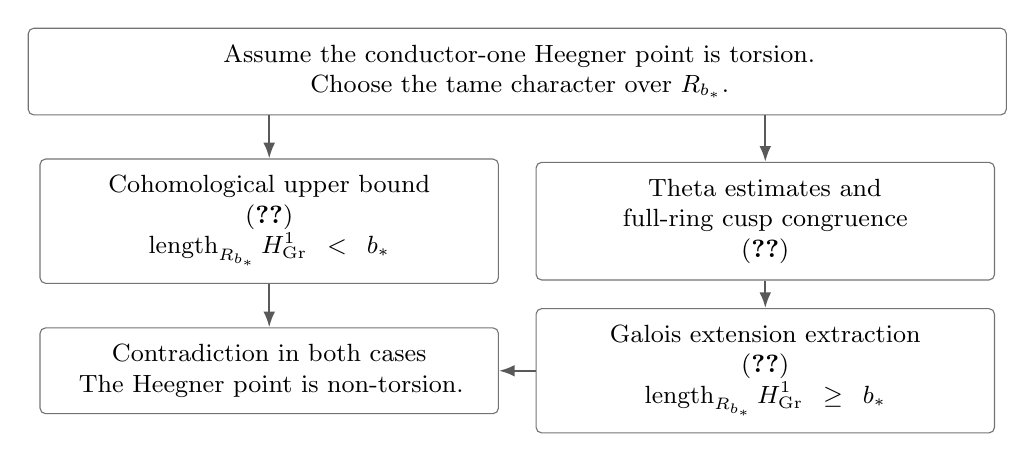
\begin{tikzpicture}[
  box/.style={draw=black!55,rounded corners=2pt,align=center,
    text width=5.4cm,minimum height=1.05cm,inner sep=6pt,font=\small},
  arr/.style={-{Latex[length=2mm]},thick,draw=black!65},
  node distance=0.65cm and 0.55cm]
 \node[box,text width=12cm] (hyp) at (0,0)
 {Assume the conductor-one Heegner point is torsion.\\
 Choose the tame character over $R_{b_*}$.};
 \node[box] (upper) at (-3.15,-1.9)
 {Cohomological upper bound\\
 (\cref{prop:green-length})\\
 $\length_{R_{b_*}}\GrH<b_*$};
 \node[box] (theta) at (3.15,-1.9)
 {Theta estimates and\\
 full-ring cusp congruence\\
 (\cref{prop:cusp-congruence})};
 \node[box] (lower) at (3.15,-3.8)
 {Galois extension extraction\\
 (\cref{prop:extension-extraction})\\
 $\length_{R_{b_*}}\GrH\ge b_*$};
 \node[box] (end) at (-3.15,-3.8)
 {Contradiction in both cases\\
 The Heegner point is non-torsion.};
 \draw[arr] (hyp.south -| upper.north) -- (upper.north);
 \draw[arr] (hyp.south -| theta.north) -- (theta.north);
 \draw[arr] (theta) -- (lower);
 \draw[arr] (upper) -- (end);
 \draw[arr] (lower) -- (end);
\end{tikzpicture}
\caption{The two bounds concern the same admissible Greenberg module
 over $R_{b_*}$. Nonzero localization gives upper bound $0$ and
 $b_*=1$; the strict case gives upper bound at most $2$ and $b_*=3$.}
\label{fig:proof}
\end{figure}


The proof therefore separates into the arithmetic reduction and
upper bound in Sections~\ref{sec:reduction}--\ref{sec:tame}, the theta
and cusp congruence in Sections~\ref{sec:theta}--\ref{sec:cusp-lifting},
and the Galois construction and extraction in
Sections~\ref{sec:parameters}--\ref{sec:extensions}.
Section~\ref{sec:sylvester} gives the cube-sum application.
The simultaneous transfer in Section~\ref{subsec:simultaneous-transfer}
uses Labesse's base-change theorem, with its sign property verified
for the holomorphic discrete series at both real places.
Appendix~\ref{sec:nonstandard-transfer} records a separate normalized
global measure comparison and a change-of-characteristic principle
for nonstandard weighted orbital integrals.

\section{Arithmetic reduction and conventions}\label{sec:reduction}

The converse at $2$ settles the even prime.  For an odd prime, we
choose auxiliary quadratic fields so that the problem reduces to
proving that one conductor-one Heegner trace is non-torsion.  The
resulting compact Selmer spaces will also supply the initial data
for the tame deformation.

\subsection{Selmer groups and established inputs}

For a number field $M$, put $T_pA_0=\varprojlim_n A_0[p^n]$ and
$V_pA_0=T_pA_0\otimes_{\Z_p}\Q_p$. For a finite place $v$ of $M$,
the finite local condition is the Kummer image
\[
 \Hf(M_v,V_pA_0)
 =\im\bigl(A_0(M_v)^{\wedge}_p\otimes_{\Z_p}\Q_p
       \longrightarrow H^1(M_v,V_pA_0)\bigr).
\]
Here $A_0(M_v)^{\wedge}_p=\varprojlim_n A_0(M_v)/p^nA_0(M_v)$.
The rational compact Selmer group is
\[
 H^1_f(M,V_pA_0)=
 \ker\left(H^1(M,V_pA_0)\longrightarrow
   \prod_v H^1(M_v,V_pA_0)/\Hf(M_v,V_pA_0)\right).
\]
Continuous cohomology and the usual archimedean local conditions are
understood. The Kummer exact sequences and local/global duality give
\begin{equation}\label{eq:compact-corank}
 \dim_{\Q_p}H^1_f(M,V_pA_0)
 =\corank_{\Z_p}\Sel_{p^\infty}(A_0/M).
\end{equation}
We use rational coefficients throughout the cohomological argument;
integral lattices will be retained whenever a uniform valuation bound
is required.

We use the following two established results.

\begin{theorem}[Established converse at $2$]
\label{thm:two-converse-input}
If $E/\Q$ is any elliptic curve and
$\corank_{\Z_2}\Sel_{2^\infty}(E/\Q)=r\in\{0,1\}$, then
\[
 \ord_{s=1}L(E,s)=\rank E(\Q)=r,
 \qquad \Sha(E/\Q)\text{ is finite}.
\]
\end{theorem}

\begin{theorem}[Established analytic twist-density theorem]
\label{thm:twist-density-input}
For any elliptic curve $E/\Q$, among nonzero squarefree integers $d$
ordered by $|d|$, the quadratic twists $E^{(d)}$ of analytic rank zero
and one each have density $1/2$. In particular the exceptional set of
twists of analytic rank at least two has density zero.
\end{theorem}

These are \citet[Theorems~1.1 and~1.2]{OpenAIGoldfeldDensity2026}.
Theorem~\ref{thm:two-converse-input} treats the prime $2$.
For auxiliary-field selection we use the density-zero exceptional-set
consequence of Theorem~\ref{thm:twist-density-input} in fixed
positive-density congruence classes.
The remainder of the paper supplies the argument at odd primes.

Fix $A_0$ and $r=s_p(A_0)\in\{0,1\}$. By
Theorem~\ref{thm:two-converse-input}, we may assume $p>2$. Write
$N$ for the conductor and $V=V_pA_0$. The Weil pairing gives
$V\simeq V^*(1)$ with alternating pairing. The $p$-parity theorem
\citep[Theorem~1.4]{DokchitserDokchitser2010} gives the global root
number
\begin{equation}\label{eq:root-sign}
 w(A_0)=(-1)^r.
\end{equation}
Modularity and the Gross--Zagier--Kolyvagin theorems will be used in
their rank-zero and rank-one forms
\citep{BCDT2001,GrossZagier1986,Kolyvagin1990}.

\subsection{Two auxiliary discriminants}

\begin{lemma}\label{lem:auxiliary-fields}
There are coprime negative odd fundamental discriminants $D,D'$ such
that every prime dividing $2Np$ splits in both quadratic fields,
\[
 \left(\frac{D}{|D'|}\right)=1,
\]
and each of $A_0^D,A_0^{D'},A_0^{DD'}$ has the smallest analytic rank
permitted by its sign. They may also be chosen so that
\[
 K=\Q(\sqrt D),\qquad F=\Q(\sqrt{DD'}),\qquad
 L=\Q(\sqrt D,\sqrt{D'})
\]
satisfy the following properties: $L/F$ is CM and unramified at every
finite prime, $L$ has only the roots of unity $\{\pm1\}$, and $L$
does not contain the CM field of $A_0$ if $A_0$ has CM.
\end{lemma}

\begin{proof}
Negative odd fundamental discriminants in any admissible fixed
congruence class have positive density. The splitting conditions at
$2Np$ are finitely many such conditions. We can exclude the finitely
many unwanted quadratic fields and then apply
Theorem~\ref{thm:twist-density-input} to choose $D$ for which $A_0^D$
has analytic rank at most one. Its rank is then minimal for its sign.

Keep $D$ fixed. The conditions on $D'$ of being coprime to $D$,
splitting $2Np$, and satisfying the displayed Jacobi-symbol condition
again contain admissible congruence classes of positive density. For
example, impose $D'\equiv-1\pmod{|D|}$ and $D'\equiv1$ at a
sufficiently divisible modulus supported on $2Np$. The moduli are
coprime, and $|D'|\equiv1\pmod{|D|}$ gives the required Jacobi
symbol. Exclude the finitely many remaining forbidden fields. Apply
the density theorem to both $A_0$ and $A_0^D$. The union of their two
exceptional sets has density zero, so some $D'$ in the prescribed
classes makes both $A_0^{D'}$ and $(A_0^D)^{D'}=A_0^{DD'}$ have
analytic rank at most one.

This use of density is unchanged if parameters are described by
fundamental discriminants: for squarefree $d$ the corresponding
discriminant is $d$ or $4d$, so a zero-density exceptional set remains
zero-density. In the odd classes used here the parameter itself is
the discriminant.

The three quadratic subfields have discriminants $D,D',DD'$.
Consequently the biquadratic discriminant formula gives
\[
 |\operatorname{disc}(L)|=D^2(D')^2
   =\operatorname{disc}(F)^2.
\]
The discriminant formula for $L/F$ therefore has relative
discriminant of norm one, proving finite unramifiedness. The two
imaginary subfields give the CM involution over the real field $F$.
The exclusions made above remove any extra roots of unity and the
possible CM field of $A_0$.
\end{proof}

\begin{proposition}\label{prop:arithmetic-reduction}
With these choices,
\[
 \dim H^1_f(K,V)=1,
 \qquad
 \dim H^1_f(K,V^{DD'})=1.
\]
The second line localizes nontrivially at both places of $K$ over $p$.
Let $y\in A_0(K)$ be the norm of the conductor-one Heegner point
under a modular parametrization taking the cusp $\infty$ to zero.
If $y$ is non-torsion, Theorem~\ref{thm:main} follows.
\end{proposition}

\begin{proof}
For a fundamental discriminant prime to $N$, the quadratic-twist
root-number formula is $w(A_0^d)=w(A_0)\chi_d(-N)$.
The splitting conditions and the signs of $D,D'$ therefore give
\[
 w(A_0^D)=w(A_0^{D'})=-(-1)^r,
 \qquad w(A_0^{DD'})=(-1)^r.
\]
By Lemma~\ref{lem:auxiliary-fields}, their analytic ranks are
$1-r,1-r,r$, respectively. Gross--Zagier--Kolyvagin gives the same
Mordell--Weil and $p$-power Selmer ranks and finite Sha for these three
twists. Restriction and corestriction for the quadratic extension
$K/\Q$ give
\[
 H^1_f(K,V)
  =H^1_f(\Q,V)\oplus H^1_f(\Q,V^D),
\]
and the analogous decomposition for $V^{DD'}$. Thus the two dimensions
are $r+(1-r)=1$ and $r+(1-r)=1$.

For the second representation both summands come from twists with
known analytic rank at most one. Its Selmer line is therefore spanned
by a non-torsion global point on the corresponding twist over $K$.
Such a point has nonzero image under the local logarithm at either
place above $p$. Indeed, on a fixed $p$-adic completion, a finite-index
open subgroup is a formal group on which the logarithm is injective
after shrinking; a point with zero logarithm consequently has a
torsion multiple in that subgroup, and is torsion. This argument uses
no reduction hypothesis.

Every prime dividing $N$ splits in $K$, so the classical Heegner
hypothesis holds. The Gross--Zagier formula identifies the nonzero
height of $y$ with simple vanishing of
\[
 L(A_0/K,s)=L(A_0,s)L(A_0^D,s)
\]
at $s=1$. Since the second factor has order $1-r$, a non-torsion $y$
implies $a(A_0)=r$. The analytic rank-zero/one theorems then give
$\rank A_0(\Q)=r$ and finiteness of the whole $\Sha(A_0/\Q)$.
\end{proof}

For the rest of the proof we assume
\begin{equation}\label{eq:torsion-assumption}
 y=0\quad\text{in }A_0(K)\otimes\Q.
\end{equation}
We will derive a contradiction. In particular, every subsequent
choice is made after $A_0,p,D,D'$ have been fixed.
The first Selmer line in Proposition~\ref{prop:arithmetic-reduction}
may have zero localization, whereas the second cannot.
Section~\ref{sec:tame} distinguishes these two possibilities before
deforming the representations.

\subsection{Coefficient, character, and measure conventions}
\label{sec:conventions}

Fix embeddings into $\C$ and $\overline{\Q}_p$. Let $\Sigma$ be the CM
type on $L$ induced from one embedding of $K$, and let $\Sigma_p$ be
the corresponding half of the places of $L$ above $p$. Complex
conjugation is denoted by $c$. All the fields introduced above are
split at $p$, and the places of $K$ above $p$ will be distinguished
according to this choice.

Smooth characters and normalized Satake parameters are evaluated on
uniformizers using the reciprocity convention corresponding to
geometric Frobenius. Write $\epsilon$ for the cyclotomic character.
A de Rham weight of $\epsilon^{-1}$ is called $1$. When a local
cohomology computation instead uses arithmetic Frobenius, this will
be stated; inversion changes neither the vanishing assertions nor
the invertibility requirements used below.

Characters of $\U(1)_{L/F}=\ker\Norm_{L/F}$ are pulled back to
characters of $L^\times\backslash\A_L^\times$ by $z\mapsto z/z^c$;
the same convention applies to $K/\Q$. Choose a character
$\mathcal C$ of $\U(1)_{K/\Q}$ with infinity type $s\mapsto s$ in
the chosen embedding and with finite conductor supported on split
primes away from $pDD'N$. These primes may be required to split
completely in $L$. The ray-class construction gives such a character:
a sufficiently deep split conductor removes the finite unit
obstruction, and the prescribed algebraic character on principal
ideles then extends across the finite ray-class quotient. We use the
same symbol for its norm pullback to $\U(1)_{L/F}$ and for the
corresponding algebraic $p$-adic character.

At the distinguished split component above $p$, its finite smooth
part has uniformizer value of valuation $-1$ with these conventions.
This records the algebraic infinity contribution; it is not a claim
that the smooth character is unitary in the $p$-adic norm. All
archimedean weights $m\to+\infty$ below also satisfy $m\to0$
$p$-adically on a fixed residue branch, including the finite torsion
orders of the characters raised to the $m$th power.

Let $k$ be a sufficiently large fixed finite extension of $\Q_p$,
with ring of integers $\cO$. We enlarge it finitely when fixed
algebraic normalization factors require this. Valuation bounds refer
to fixed bases and integral lattices. A \emph{uniform} bound may
depend on the fixed data and on a fixed truncation degree, but not on
the moving prime, its growing $p$-power quotient, or the growing
weights. When coefficient fields for classical eigensystems vary,
we retain their embeddings in $\overline{\Q}_p$ and use valuation
bounds; no compactness of their union is assumed.

For an algebraic group $H$ over a number field $M$, write
$[H]=H(M)\backslash H(\A_M)$.

Measures on compact source groups and archimedean integration tori
have algebraic normalization, and maximal compact subgroups have
volume one at almost every finite place. Passing between these
measures and invariant norm formulas costs a fixed global scalar.
All toric sums called \emph{raw} below are sums without division by
the varying ring-class order. This distinction is essential for
the estimates at the moving primes.

\section{A tame deformation and its Selmer length}\label{sec:tame}

We retain the fields and the contradiction assumption of
\cref{sec:reduction}.  In particular, the conductor-one Heegner trace
$y\in A_0(K)$ is torsion.  Put $T=T_pA_0$ and
$V=T\otimes_{\Z_p}\Q_p$.  Initially all cohomology in this section has
$\Q_p$ coefficients; extension to the fixed finite coefficient field
$k$ is made by tensor product.  Enlarge the finite, conjugation-stable
set $S$ to contain the places over $p$, the bad places of $A_0$, and all
the fixed conductors used below.  It may be enlarged by a further
\emph{fixed} finite set at any stage.  In particular, the auxiliary
finite characters and tests of Section~\ref{sec:content} are chosen
independently of the moving primes, and their conductors are included
before the final prime sequence is realized.  All the constructions
below allow this fixed enlargement.  Write $G_{K,S}$ for the Galois
group unramified outside $S$.

We need two conclusions for the same tame deformation.  The
one-sided local condition, full at one $p$-adic place and zero at
its conjugate, will give a cohomology module of length zero or at
most two.  Under the torsion assumption on $y$, the first one or
three coefficients of the corresponding weighted Heegner logarithms
will tend to zero, respectively.  These are
\cref{prop:green-length,prop:heegner-log}.  The logarithm estimate
supplies the constant-term estimate of
\cref{prop:constant-term-small}; the length bound will contradict
the extensions extracted in Section~\ref{sec:extensions}.

\subsection{The undeformed Selmer spaces at the two places above \texorpdfstring{$p$}{p}}

The two places $v,v^c$ of $K$ above $p$ have completion $\Q_p$.
The alternating Weil pairing
\[
 e:V\times V\longrightarrow\Q_p(1)
\]
and the local invariant give a symmetric perfect pairing on
$H^1(K_w,V)$: the sign from interchanging two degree-one cochains
cancels the sign of $e$.  The local Kummer line
$H^1_f(K_w,V)$ is its own orthogonal complement.  Thus, for $w\mid p$,
this is a hyperbolic plane.  These statements include arbitrary
reduction at $p$: local torsion is finite, the rational Kummer space
has dimension one, and the local Euler characteristic gives
$\dim H^1(K_w,V)=2$.  At a finite place $w\nmid p$ we instead have
\begin{equation}\label{eq:away-p-vanishing}
 H^0(K_w,V)=H^2(K_w,V)=H^1(K_w,V)=0.
\end{equation}
Indeed $H^0=0$ by finiteness of local torsion, $H^2=0$ by local
duality, and the Euler characteristic away from $p$ is zero.
We use the local and global duality sequences in
\cite[Chapter~I, Sections~2--4]{Milne1986} and
\cite[Section~8.6]{NSW2008}.

For the moment let $W$ denote either $V$ or its twist $V^{DD'}$ over
$K$.  Its compact Selmer space has dimension one by
\cref{prop:arithmetic-reduction}.  Let $H^1_{\mathrm{rel}}(K,W)$ have full
conditions at $v,v^c$, and the usual unramified conditions outside
$S$; conditions at the other places of $S$ make no difference by
\cref{eq:away-p-vanishing}.  Let $H^1_{\Gr}(K,W)$ have full condition
at $v$ and zero condition at $v^c$, and let
$H^1_{\overline{\Gr}}(K,W)$ have the opposite conditions.
These are the two one-sided Greenberg conditions.

\begin{lemma}\label{lem:base-green}
If the compact Selmer line of $W/K$ has nonzero localization, then
$H^1_{\Gr}(K,W)=H^1_{\overline{\Gr}}(K,W)=0$.
The only remaining possibility is the following \emph{strict case}
in the $V$ summand: $r=1$, and the compact Selmer space is generated
by a class $a$ such that $a^c=a$ and every localization of $a$ is zero.
In that case
\begin{equation}\label{eq:base-green-bases}
 H^1_{\Gr}(K,V)=\langle a,h\rangle,
 \qquad
 H^1_{\overline{\Gr}}(K,V)=\langle a,h^c\rangle,
\end{equation}
where $h$ has nonzero localization at $v$ and zero localization at
$v^c$.  The $V^{DD'}$ summand always has zero Greenberg space.
\end{lemma}

\begin{proof}
Let $F_w=H^1_f(K_w,W)$ and let $Q_w=H^1(K_w,W)/F_w$.
Poitou--Tate duality identifies the image of
\[
 H^1_{\mathrm{rel}}(K,W)\longrightarrow Q_v\oplus Q_{v^c}
\]
with the annihilator of the localization of the compact Selmer line
in $F_v\oplus F_{v^c}$.  If that localization is nonzero, both of its
coordinates are nonzero: the one-dimensional global space is stable
under $c$, which interchanges the two places.  Its annihilator is
therefore a line whose two coordinates are both nonzero for every
nonzero vector.  A class satisfying a zero condition at one place
has zero singular image, hence belongs to the compact Selmer line;
the zero condition then kills that line as well.

Suppose the compact Selmer line is everywhere locally zero.  The
same duality sequence makes the singular image all of
$Q_v\oplus Q_{v^c}$.  The kernel of localization is precisely the
compact Selmer line.  Consequently the relaxed local image has
dimension two and maps isomorphically to the singular plane.
In each local hyperbolic plane choose the isotropic complement $E_w$
of $F_w$, choosing the two complements compatibly with $c$.  The
relaxed local image is the graph of a map
\[
 E_v\oplus E_{v^c}\longrightarrow F_v\oplus F_{v^c}.
\]
Global reciprocity makes the graph isotropic.  In mutually dual
bases its matrix is therefore skew-symmetric, hence of the form
$\left(\begin{smallmatrix}0&u\\-u&0\end{smallmatrix}\right)$.
Conjugation interchanges both pairs of basis vectors and preserves
the local pairings.  Invariance of the graph therefore changes $u$
to $-u$, so $u=0$.  Lifting the first coordinate line gives $h$;
conjugating gives $h^c$ and proves \cref{eq:base-green-bases}.

The auxiliary summand has a nontorsion global point and nonzero
localization, by \cref{prop:arithmetic-reduction}.  If $r=0$, the unique
Selmer line of $V/K$ likewise comes from a nontorsion point on the
quadratic twist $A_0^D/\Q$, so it cannot be strict.  When $r=1$, the
twist by $D$ has zero Selmer space and the line comes from
$H^1_f(\Q,V)$, giving $a^c=a$.
\end{proof}

\subsection{Primes with a controlled tame logarithm}

In the prime construction and cohomological calculations of this section,
Galois Frobenius elements are arithmetic Frobenius elements.
The following construction gives a tame direction that is trivial at
the fixed places and has uniform local bounds.  In the strict case
we will refine its limiting Frobenius element after determining the
obstruction to first-order lifting.

\begin{proposition}\label{prop:tame-primes}
There are rational primes $q_i\notin S$, split completely in $L$,
distinguished places $\mathfrak q_i$ of $K$ above them, cyclic
$p$-quotients $\Delta_i$ of the ring class group of conductor $q_i$,
and surjections
\[
 \ell_i:G_K\longrightarrow\Delta_i\simeq\Z/p^{n_i}\Z,
 \qquad n_i\longrightarrow\infty,
\]
with the following properties.
\begin{enumerate}[label=\textup{(\roman*)}]
\item $\ell_i$ is unramified outside the pair above $q_i$,
its restriction to inertia at $\mathfrak q_i$ is surjective,
$\ell_i^c=-\ell_i$, and $\ell_i|_{G_{K_s}}=0$ for every $s\in S$.
\item $v_p(q_i-1)-n_i$ is bounded.  At either place above $p$, the
full ring class field of conductor $q_i$ is unramified and its local
degree has bounded $p$-part.
\item Frobenius at $\mathfrak q_i$, on all fixed data unramified
outside $S$, tends to an element $\gamma\in G_L$ such that
\[
 \eps(\gamma)=1,\qquad
 \det(V(\gamma)-1)\ne0,\qquad
 \cC(\gamma)\text{ is not a root of unity}.
\]
Moreover $\gamma$ fixes all $p$-power radicals of a fixed,
conjugation-stable finite list in $K^\times$ spanning
$\cO_{K,S}^{\times}\otimes\Q_p$ under the Kummer map.
\end{enumerate}
\end{proposition}

\begin{proof}
Choose representatives $\mathfrak a_j$ for generators of the ideal
class group, prime to $S$.  For their orders, their multiplication
relations, and the expressions of the primes in $S$ in these
generators, choose principal generators.  Adjoin generators of the
finite-rank $S$-unit group and their conjugates to this finite list,
denoted $\alpha_1,\ldots,\alpha_d$.  Fixed class-group orders and
roots of unity will cost only a fixed index.

For a split prime $q$, the kernel of the ring class group map to the
ordinary ideal class group is the quotient of
$(\cO_K/q\cO_K)^\times$ by diagonal residue units and global units.
Its $p$-part is cyclic, of order $p^{v_p(q-1)}$ up to a fixed factor.
Require the $\alpha_j$ to have zero residue logarithm modulo
$p^{n_i}$ at the pair over $q_i$.  This is ensured by splitting in
their $p^{n_i}$-radical extensions, together with the corresponding
roots of unity.  The ring class presentation now allows us to set
the logarithms of all $\mathfrak a_j$ equal to zero and to take the
surjective logarithm on the residue quotient.  Each relation is
respected, and the expressions chosen for the primes of $S$ give
$\ell_i|_{G_{K_s}}=0$.  Conjugation inverts the residue quotient and
the ring class action, giving $\ell_i^c=-\ell_i$.

We verify that imposing the full radical condition leaves room for
$\gamma$.  Over the cyclotomic tower the Kummer Galois group is a
closed subgroup of $\Z_p(1)^d$.  The joint image of $V$ and $\cC$
is a $p$-adic Lie group.  A common Lie quotient with this translation
group is abelian, so it kills the derived Lie algebra of the image
of $V$.  On the remaining torus Lie algebra, conjugation by an open
cyclotomic subgroup is trivial; on the Kummer translations it is
multiplication by the cyclotomic character.  Any equivariant common
quotient is consequently zero.  This argument can be made after a
fixed finite extension, which does not change Lie dimensions.
Thus killing the radicals removes no Lie dimension from the joint
image over the cyclotomic tower.

For a non-CM elliptic curve the determinant-one image has Lie
algebra $\mathfrak{sl}_2$, by the open image theorem
\cite{Serre1972}; for a CM curve its identity component contains
the norm-one torus, by the CM description of the Tate-module
character \cite{Serre1968}.  In either
case the locus $\det(V(g)-1)\ne0$ is nonempty and open in every
sufficiently small identity neighborhood.  The infinity type of
$\cC$ makes its restriction over the cyclotomic tower nonconstant;
its torsion locus is a proper closed subset in a sufficiently small
identity neighborhood.  The two complements intersect.  We may
also impose $g\in G_L$ and any fixed open-kernel conditions.  This
gives $\gamma$ fixing the full radicals and the cyclotomic tower
with the required properties.

It remains to control $v_p(q_i-1)$, rather than merely make it
large.  The cyclotomic--radical image is a closed subgroup of
\[
 \Z_p(1)^d\rtimes\Z_p^\times
\]
with open cyclotomic projection.  Choose an element in a pro-$p$
subgroup whose cyclotomic projection is nontorsion.  Its $p^m$-th
powers tend to the identity; their translation coordinates are
divisible by $p^{m-C_0}$, and the valuation of their cyclotomic
coordinate minus one is $m+C_1$, for fixed $C_0,C_1$.  Multiplying
$\gamma$ by such a power with $m=n_i+C_2$ therefore leaves all
radicals trivial modulo the requested precision and makes the
cyclotomic valuation exactly $n_i+C$, for a fixed $C$.  Chebotarev
applied to a growing sequence of finite quotients realizes these
conditions and increasingly accurate approximations on all fixed
data.  Choosing a place above each prime selects the indicated
Frobenius representative.  The primes can be taken outside any
fixed finite set.

Finally the $p$-part of the order of the full ring class group is
$p^{v_p(q_i-1)+O(1)}$.  The kernel of its map to $\Delta_i$ therefore
has bounded $p$-part.  The Frobenius of every $s\in S$ belongs to this
kernel.  At $p$ the extension is unramified, so the $p$-part of the
local degree, which is the $p$-part of the Frobenius order, is
bounded.  This proves the proposition.
\end{proof}

\subsection{Admissible cochains and division by the parameter}

Fix a nonprincipal ultrafilter $\cU$ on the prime indices.  A
statement ``eventually'' in the construction below means on a set
in $\cU$.  For every fixed $b\ge1$, put
\[
 R_b=k[t]/(t^b).
\]
At finite stages the substitution of $(1+t)^{\ell_i}$ is defined
only to finite $p$-adic precision.  There is a constant $c_b$ such that
\begin{equation}\label{eq:binomial-loss}
 u\equiv u'\pmod {p^n}\quad\Longrightarrow\quad
 \binom{u}{j}\equiv\binom{u'}{j}\pmod {p^{n-c_b}}
 \quad(0\le j<b).
\end{equation}
This follows by writing each binomial coefficient as a polynomial
with denominator $j!$.  Thus truncated substitution of
$(1+t)^{\ell_i}$ defines an action modulo $p^{n_i-c_b}$ and sends
integral group-ring elements of $\Delta_i$ to coefficients with a
fixed denominator.  No division by $|\Delta_i|$ is involved.

For a sequence $(g_i)$, let $\ell((g_i))$ be the $p$-adic ultralimit
of $\ell_i(g_i)\in\Z/p^{n_i}\Z$: each fixed residue modulo $p^m$ is
well-defined eventually and has a unique ultralimit.  This is an
additive character on the group of sequences of elements of
$G_{K,Sq_i}$, modulo equality on a set in $\cU$.  We can therefore
define
\[
 \psi=(1+t)^\ell,\qquad
 M_b^{\eta}=V\otimes_{\Q_p}R_b(\psi^{\eta}),
 \qquad \eta\in\{1,-1\}.
\]
Constant representations have their usual compact $p$-adic ultralimit.

\begin{definition}\label{def:admissible}
An \emph{admissible cochain} with coefficients in $M_b^{\eta}$ is a
function on sequences of Galois elements which is the coefficientwise
ultralimit of continuous finite-stage cochains, in the fixed basis
of $V\otimes R_b$, with one denominator $p^C$ independent of $i$.
Finite-stage cochain identities are required modulo precisions
$A_i\longrightarrow\infty$ along $\cU$, with
$A_i\le n_i-c_b$.  Equivalently, the limiting identity holds on
\emph{every} sequence of arguments.  Cohomology is the cohomology
of this cochain complex, so coboundaries are also required to be
admissible.  Local complexes are defined by the chosen embeddings
of decomposition groups.  The same definition applies over $L$ by
restriction and inverse image of the finite-stage Galois groups.
\end{definition}

The equivalence in the definition uses boundedness: if an identity
failed uniformly modulo $p^m$ on a set in $\cU$, choosing one
violating tuple at every such index would violate the identity on
that sequence.  A diagonal choice of precisions then gives
$A_i\to\infty$.  This observation also applies when replacing two
cochain systems with the same limit.  In particular, pointwise
agreement only on fixed Galois elements would not suffice.

\begin{lemma}\label{lem:admissible-specialization}
For constant coefficients $V$, admissible $H^1$ is precisely
$H^1(G_{K,S},V)$, and likewise over $L$.  For $\Q_p(1)$ the same
assertion holds when unramifiedness at the moving primes is imposed.
The fixed local conditions specialize to the usual rational local
conditions.  Coefficient reduction and multiplication by $t$ give
short exact sequences of admissible cochain complexes
\begin{equation}\label{eq:coefficient-sequence}
 0\longrightarrow C^\bullet(M_{b-1}^{\eta})
 \xrightarrow{\ t\ } C^\bullet(M_b^{\eta})
 \longrightarrow C^\bullet(V\otimes k)\longrightarrow0.
\end{equation}
Zero local conditions at $p$ and local Kummer conditions are
preserved by the resulting division of a class with zero
specialization by $t$.
\end{lemma}

\begin{proof}
Choose a stable lattice in $V$.  A bounded finite-stage cocycle
modulo $p^{A_i}$ has trivial wild inertia at $q_i$.  On tame
$p$-inertia the Frobenius relation implies
\[
 (V(\Frob_i)-q_i)z_i(\tau)=0\pmod {p^{A_i-C}}.
\]
The inverses of $V(\Frob_i)-q_i$ have a fixed denominator: these
matrices converge to the invertible matrix $V(\gamma)-1$.
The same is true at the conjugate prime and over $L$.  After one
fixed loss of precision, the cocycle kills the normal subgroup
generated by moving inertia, hence factors through $G_{K,S}$.
For each fixed finite coefficient module, there are only finitely
many continuous cocycles on $G_{K,S}$: cohomological finiteness
follows from the finiteness of extensions with fixed ramification
and bounded degree, and the group of coboundaries is finite.
Taking the compatible ultralimits of these finite sets yields an
actual continuous integral cocycle; then undo the fixed scaling.
For cyclotomic coefficients the proof is the same once moving
inertia has been required to vanish.  Equality of classes is
compatible with this procedure because bounded zero-cochains
have compact ultralimits.  It also shows that a representative of
a given ordinary class can be replaced by a chosen continuous
representative, up to a bounded coboundary and uniformly vanishing
errors.

Exactness of \cref{eq:coefficient-sequence} is coefficientwise:
lift the finitely many coordinates continuously, and divide a
zero constant coefficient by $t$ by shifting coordinates.  These
operations do not enlarge a uniform denominator except for the
fixed truncation loss in \cref{eq:binomial-loss}.  The character is
exactly trivial at the fixed places in $S$, so there
\[
 H^1(K_s,M_b^{\eta})=H^1(K_s,V\otimes k)\otimes_k R_b,
 \qquad
 H^1_f(K_s,M_b^{\eta})=H^1_f(K_s,V\otimes k)\otimes_k R_b.
\]
These are fixed linear subspaces.  A strictly zero local class
can be made a zero local cocycle with bounded corrections: since
$H^0(K_s,V)=0$, finitely many elements $g_1,\ldots,g_u$ make
\[
 V\longrightarrow V^u,\qquad
 A\longmapsto((V(g_j)-1)A)_j
\]
injective.  A fixed left inverse bounds the denominator of every
such correction.  Therefore division preserves the strict and
Kummer conditions, both in rational cohomology and in their
finite-precision representatives.
\end{proof}

Over $L$ we impose full local conditions at the places of
$\Sigma_p$, zero conditions at their conjugates, and relaxed
conditions at the other places of $S$.  This is the notation
$\GrH(L,M_b^{\eta})$ used below, always with admissible cohomology.
Restriction, the two idempotents for $\Gal(L/K)$, and corestriction
decompose it into the corresponding spaces for $V$ and $V^{DD'}$
over $K$.  Their denominators are fixed (in fact $2$ is a unit).
Thus all length computations may be made over $K$.

\subsection{The first-order obstruction}

We now work in the strict case of \cref{lem:base-green}.  Choose
fixed continuous cocycles for $a,h,h^c$, taking the representatives
equivariantly under $c$ by averaging.  Cup products below contract
with $e$, and $\delta$ denotes the cochain differential.

Let $x$ be a fixed cocycle representing a class in
$H^1_{\Gr}(K,V)$.  A first-order lift has the form $x+t x_i'$.
Comparing the coefficients of $t$ in its cocycle
equation gives
\begin{equation}\label{eq:linear-lift}
 \delta x_i'=-\eta\ell_i\cup x
\end{equation}
modulo precision tending to infinity.  To obstruct a lift with the
Greenberg local conditions, we pair this equation with a class
having the opposite local conditions.  The proof below justifies
the bounded corrections needed to use the fixed representative $x$.

For $d\in H^1_{\overline{\Gr}}(K,V)$, the
product $x\cup d$ vanishes at every place: at $p$ one of the two
classes is zero, and away from $p$ use
\cref{eq:away-p-vanishing}.  The injection of global degree-two
cyclotomic cohomology into its localizations (Brauer reciprocity)
gives a continuous cochain $u$ on $G_{K,S}$ satisfying
\begin{equation}\label{eq:cup-primitive}
 \delta u=x\cup d.
\end{equation}
Choose primitives for the finitely many pairs in the two fixed
bases, and thereafter use bilinear extension.  Each has compact
image, hence all these choices have one fixed denominator.

For an element $\gamma$ as in \cref{prop:tame-primes}, define
\begin{align}
 z_\gamma(x,d;u)
 &=u(\gamma)-e\bigl((V(\gamma)-1)^{-1}x(\gamma),d(\gamma)\bigr),
 \label{eq:corrected-primitive}\\
 H_\gamma(x,d)
 &=z_\gamma(x,d;u)-z_\gamma(x^c,d^c;u^c).
 \label{eq:obstruction-pairing}
\end{align}
The chosen trivialization of $\Q_p(1)$ makes these scalar
expressions; changing it multiplies them by one nonzero scalar.

\begin{lemma}\label{lem:obstruction-necessary}
The expression $H_\gamma$ is independent of the primitive and
bilinear.  If a nonzero class $x\in H^1_{\Gr}(K,V\otimes k)$ is the
specialization of an admissible class in
$\GrH(K,M_2^{\eta})$, then
\begin{equation}\label{eq:obstruction-vanishing}
 H_\gamma(x,d)=0
 \quad\text{for every }d\in H^1_{\overline{\Gr}}(K,V\otimes k).
\end{equation}
The same necessary condition holds for either $\eta$.
\end{lemma}

\begin{proof}
We give the finite-precision argument, so that no continuity
assertion about the varying Galois groups is implicit.  For
$\eta=1$, write a first-order lift as $x+t x_i'$ satisfying
\cref{eq:linear-lift}.  Indeed,
\cref{lem:admissible-specialization} permits subtraction of one
bounded global coboundary and replacement of its constant
coefficient by the chosen fixed cocycle $x$.  Equality on all
sequences makes the error uniformly small.  Its linear coefficient
remains bounded.  The cochain
\begin{equation}\label{eq:global-two-cocycle}
 x_i'\cup d-\ell_i\cup u
\end{equation}
is consequently a two-cocycle modulo the reduced precision.
Its local invariants at $S$ vanish to increasing precision.  At
$p$ this follows from opposite strict conditions and $\ell_i=0$;
away from $p$ it follows from the vanishing of rational $H^1$ and
the bounded exponents of the fixed integral local cohomology
groups.  At places outside $S q_i$ it is unramified and has zero
invariant.

At $\mathfrak q_i$, the fixed cocycles $x,d$ are unramified and
are coboundaries, say $x=\delta A_i$, $d=\delta B_i$, where
\[
 A_i=(V(\Frob_i)-1)^{-1}x(\Frob_i),\qquad
 B_i=(V(\Frob_i)-1)^{-1}d(\Frob_i).
\]
These vectors have bounded denominators, because the inverse
matrices converge to $(V(\gamma)-1)^{-1}$.  By
\cref{eq:linear-lift}, $x_i'-\ell_i\cup A_i$ is a cocycle.
Its cup product with $d$ is a coboundary.  The invariant of
\cref{eq:global-two-cocycle} therefore equals minus the invariant
of
\begin{equation}\label{eq:tame-corrected-cup}
 \ell_i\cup(u-A_i\cup d).
\end{equation}
The second factor is an unramified cyclotomic one-cocycle locally,
since its differential is $x\cup d-(\delta A_i)\cup d=0$.
The tame local pairing evaluates this unramified factor at
Frobenius and pairs it with the inertia logarithm.  With compatible
local invariant conventions, the multiplier at stage $i$ is a unit
$\nu_i$ modulo the working precision, because the logarithm on tame
inertia is surjective.  At the conjugate prime the same calculation
uses $x^c,d^c,u^c$ and $\ell_i^c=-\ell_i$; functoriality of the local
invariant gives the same multiplier $\nu_i$.  Choose unit lifts to
$\Z_p$ and let $\nu\in\Z_p^\times$ be their compact ultralimit.
The global sum of invariants then gives $\nu H_\gamma(x,d)=0$,
hence \cref{eq:obstruction-vanishing}.  This calculation never
divides by $q_i-1$.  We use arithmetic Frobenius
in this calculation; replacing it throughout by geometric
Frobenius changes the conventions compatibly and not the zero
condition.  For $\eta=-1$, replace $\ell_i$ by $-\ell_i$.

Here is the precise bound on all reductions of precision.  Let
$c_{\mathrm{fix}}$ bound the fixed cocycles and their finitely many
primitives, and let $c_{\mathrm{lift}}$ bound the particular
admissible lift.  Let $c_\gamma$ clear both inverses
$V(\Frob_i)-1$ and $V(\Frob_i)-q_i$ eventually.  Let $c_S$ bound
the fixed left inverses detecting local $H^0=0$ and the exponents
of integral $H^1,H^2$ at the fixed places away from $p$.  Finally
use the binomial constant $c_b$ of \cref{eq:binomial-loss}.
All displayed corrections use finitely many sums and products of
these objects.  A constant
$C=C(c_{\mathrm{fix}},c_{\mathrm{lift}},c_\gamma,c_S,c_b)$ therefore
bounds every loss.  If the original cochain identities hold to
precision $A_i$ and their replacement accuracies are $B_i$, make
the calculation to any precision
\begin{equation}\label{eq:precision-choice}
 N_i\le\min\{n_i,A_i,B_i\}-C,\qquad N_i\longrightarrow\infty.
\end{equation}
The tame pairing above is defined at this precision since
$N_i\le n_i$.  The constants may depend on a fixed lift and on
$b$, but never on $i,q_i,n_i$.  Only finitely many fixed primitives
were chosen; no bounded contracting homotopy on all cochains is
being asserted.

For independence of $u$, the difference of two primitives is in
\[
 H^1(G_{K,S},\Q_p(1))
   =\cO_{K,S}^{\times}\otimes_{\Z}\Q_p.
\]
The equality is the Kummer sequence and finiteness of the
$S$-class group.  The radical list in \cref{prop:tame-primes}
spans this space, including its conjugate, up to a fixed index.
Every such Kummer class evaluates to zero at $\gamma$; a
coboundary also evaluates to zero because $\eps(\gamma)=1$.
Changing $u$ therefore changes neither term of
\cref{eq:obstruction-pairing}.  Bilinearity follows from the fixed
bilinear choices of primitives.
\end{proof}

\begin{lemma}\label{lem:nonzero-obstruction}
The element $\gamma$ in \cref{prop:tame-primes} can be chosen so
that, in the bases of \cref{eq:base-green-bases}, the obstruction
matrix is
\begin{equation}\label{eq:obstruction-matrix}
 \begin{pmatrix}0&\kappa\\-\kappa&0\end{pmatrix},
 \qquad \kappa\in\Q_p^\times.
\end{equation}
Thus no nonzero base Greenberg class lifts to order two.
\end{lemma}

\begin{proof}
First $H_\gamma(x,d)=H_\gamma(d,x)$ whenever the pairs under
consideration have locally zero cup product.  To check the sign
explicitly, put $q(g)=e(x(g),d(g))$.  The cocycle identities give
\[
 \delta q=d\cup x-x\cup d,
\]
so $u+q$ is a primitive for the switched cup product.  At a place
where $x=\delta A$ and $d=\delta B$, the difference between the two
corrected evaluations is
$(\eps(\gamma)-1)e(A,B)=0$.  This proves the symmetry for the
expression in \cref{eq:corrected-primitive}, and hence for $H$.
Its definition also gives
$H_\gamma(x^c,d^c)=-H_\gamma(x,d)$.  Since $a^c=a$ and $p>2$,
these identities give both diagonal zeros in
\cref{eq:obstruction-matrix} and the opposite signs of its
off-diagonal entries.

It remains to make $\kappa=H_\gamma(a,h^c)$ nonzero.  Set
$d^-=h^c-h$.  It is anti-invariant, and its cup product with $a$
is everywhere locally zero.  Average a primitive to be
anti-invariant as well.  Then
\[
 H_\gamma(a,d^-)=2z_\gamma(a,d^-;u),\qquad
 H_\gamma(a,d^-)=2H_\gamma(a,h^c).
\]
It is enough to make $z_\gamma(a,d^-;u)$ nonzero.

Let $G=G_{K,S}$ and $N_V=\ker(G\to\GL(V))$.  The classes $a,d^-$
are linearly independent: the former is nonzero and invariant
under $c$, whereas the latter is anti-invariant with nonzero local
image.  The image of $G$ on $V$ contains a central scalar different
from one.  The usual central-scalar argument gives
$H^1(\im(G\to\GL(V)),V)=0$: for a cocycle $f$ and a central
scalar $z\ne1$, the cocycle identity is
$(z-1)f(g)=(g-1)f(z)$, so $f$ is a coboundary.
Inflation--restriction thus makes restriction to
$N_V$ injective on $H^1(G,V)$.  On $N_V$, both cocycles are additive
homomorphisms.  Their joint image spans $V\oplus V$: its span is a
$G$-submodule, and absolute irreducibility with
$\End_G(V)=\Q_p$ says that a proper submodule projecting onto each
factor would impose a scalar linear relation between the two
restrictions.  That contradicts the preceding injectivity.
The absolute irreducibility here follows from open image in the
non-CM case; in the CM case it follows because neither $K$ nor $L$
contains the CM field.  Passing to the finite-index subgroup over
$L$ leaves the span unchanged.

The Weil pairing implies $\eps=1$ on $N_V$.  On this group,
\cref{eq:cup-primitive} reads
\[
 u(gg')=u(g)+u(g')-e(a(g),d^-(g')).
\]
Consequently
\begin{equation}\label{eq:heisenberg-commutator}
 u([g,g'])=-e(a(g),d^-(g'))+e(a(g'),d^-(g)).
\end{equation}
The alternating form on $V\oplus V$ on the right is nonzero and
nondegenerate.  Since the joint translations span $V\oplus V$,
some $g,g'\in N_V\cap G_L$ have a nonzero right-hand side.
Write $\sigma=[g,g']$.  Both translations vanish on $\sigma$, but
$u(\sigma)\ne0$.

Every Kummer character in our radical list is an additive
homomorphism on $N_V$, because $\eps=1$ there.  It therefore
vanishes on $\sigma$, so $\sigma$ fixes all the radicals.  A
one-dimensional character such as $\cC$ also kills $\sigma$.
Replacing $\gamma$ by $\gamma\sigma^m$, for an integer $m$, thus
preserves its $V$, $\cC$, cyclotomic, and radical values.  The two
translations entering the correction in
\cref{eq:corrected-primitive} do not change, whereas its primitive
value changes by $m u(\sigma)$.  Some $m$ makes the result nonzero.
If further fixed open conditions are required, first replace
$\sigma$ by a suitable nonzero power; its nonzero primitive value
survives.  This constructs the required $\gamma$.  In particular
the inverse matrix $V(\gamma)-1$, and hence its denominator bound,
is unchanged by the modification.  Applying the prime construction
to this element proves \cref{eq:obstruction-matrix} for both signs
of the tame twist.
\end{proof}

In the strict case we henceforth use this refined $\gamma$ in
\cref{prop:tame-primes}, and $q_i,\ell_i$ denote the sequence
realized from it.  With the same ultrafilter $\cU$, we henceforth
form $\ell$, $\psi$, $M_b^\eta$, and the admissible global and local
cochain complexes from this reselected sequence.  The preserved
properties of the prime construction ensure that the specialization,
division, and obstruction arguments above still apply.
As stipulated at the start of the section, the
final realization is made after all fixed conductors and tests have
been chosen.  Any additional fixed open-kernel conditions can be imposed
in the construction and preserved by the commutator modification.

\subsection{The exact Artin length bound}

\begin{proposition}\label{prop:green-length}
For the primes of \cref{prop:tame-primes}, chosen in the strict case
as in \cref{lem:nonzero-obstruction}, every fixed $b\ge1$, and
either $\eta=1$ or $\eta=-1$, one has
\begin{equation}\label{eq:green-length}
 \length_{R_b}\GrH(L,V\otimes\psi^{\eta})
 \begin{cases}
 =0,&\text{outside the strict case},\\
 \le2,&\text{in the strict case}.
 \end{cases}
\end{equation}
In the strict case this module is killed by $t$ and is the image
of its two-dimensional base space under multiplication by
$t^{b-1}$.  Put
\begin{equation}\label{eq:b-star}
 b_*=1\quad\text{outside the strict case},\qquad
 b_*=3\quad\text{in the strict case}.
\end{equation}
Thus in both cases the length in \cref{eq:green-length} is
strictly smaller than $b_*$.
\end{proposition}

\begin{proof}
It suffices to work in each of the two summands over $K$.
Let $\mathcal S_b^\bullet$ be the cone, shifted by $-1$, of the
map from the admissible global cochain complex to the local
complex at the strict $p$-place.  Its degree-one cohomology is
exactly the indicated Greenberg group.  Indeed global and local
$H^0$ vanish for $V$ and, by the $t$-filtration, for every $M_b$.
The coefficient sequence in \cref{eq:coefficient-sequence} gives a
short exact sequence of these cone complexes.  The resulting
cohomology sequence therefore identifies
\begin{equation}\label{eq:selmer-kernel}
 \ker\bigl(H^1(\mathcal S_b^\bullet)
       \longrightarrow H^1(\mathcal S_1^\bullet)\bigr)
 =\im\bigl(t:H^1(\mathcal S_{b-1}^\bullet)
       \longrightarrow H^1(\mathcal S_b^\bullet)\bigr).
\end{equation}
There is no flatness assumption on these cohomology groups.

If the base group is zero, induction in \cref{eq:selmer-kernel}
gives zero at every order.  This deals with the auxiliary summand
and with both summands outside the strict case.  In the strict
summand, a class at any order $b\ge2$ reduces to an order-two
class, whose base specialization is zero by
\cref{lem:obstruction-necessary,lem:nonzero-obstruction}.
Equation~\eqref{eq:selmer-kernel}, iterated, gives
\[
 H^1(\mathcal S_b^\bullet)
   =\im\bigl(t^{b-1}:H^1(\mathcal S_1^\bullet)
                    \longrightarrow H^1(\mathcal S_b^\bullet)\bigr).
\]
This image is killed by $t$ and has $k$-dimension at most two.
Its $R_b$-length is therefore at most two, as asserted.
\end{proof}

\subsection{A uniform local logarithm estimate}

The cohomological length bound is now proved.  Under the torsion
assumption on $y$, we next establish the weighted Heegner-logarithm
vanishing needed for the theta congruence.  The argument first gives
vanishing of local Kummer classes.  The following estimate converts
this into a valuation statement, uniformly in the unramified fields
of definition that occur at $p$.

\begin{lemma}\label{lem:uniform-local-log}
Fix an integer $d_0\ge0$.  There is a constant $c$ such that, for
every finite unramified extension $E/\Q_p$ with
$v_p([E:\Q_p])\le d_0$,
\begin{equation}\label{eq:uniform-local-log}
 \log_{A_0,p}(A_0(E))\subseteq p^{-c}\cO_E.
\end{equation}
If $P\in A_0(E)$ and the Kummer class of $p^C P$ vanishes in
$H^1(E,A_0[p^n])$, where $C,n\ge0$ are integers, then
\[
 v_p(\log_{A_0,p}P)\ge n-C-c.
\]
\end{lemma}

\begin{proof}
On a fixed sufficiently small formal subgroup, the formal logarithm
and its inverse are integral, uniformly under unramified base
extension.  The intervening formal-group quotient has bounded
$p$-exponent.  In the N\'eron special fiber the geometric component
group has fixed order, the additive part has bounded $p$-exponent,
and a torus in characteristic $p$ has no $p$-torsion.  For the
\'etale $p$-power torsion in the abelian part, let $\alpha$ be a
unit Frobenius eigenvalue.  It is not a root of unity, by its
complex absolute value.  If $[E:\Q_p]=d$, the exponent is
controlled by $v_p(\alpha^d-1)$.  Writing $\alpha$ as its finite
torsion part times a principal unit shows
\[
 v_p(\alpha^d-1)\le C_\alpha+v_p(d)
\]
whenever the left side is positive.  It is therefore bounded for
these extensions.  A fixed $p$-power, followed if necessary by an
integer prime to $p$, moves any point into the formal subgroup.
Dividing its logarithm by that multiplier proves
\cref{eq:uniform-local-log}, including at bad reduction.

For the precision assertion, the Kummer injection
\[
 A_0(E)/p^n A_0(E)\hookrightarrow H^1(E,A_0[p^n])
\]
gives $p^C P=p^n Q$ for some $Q\in A_0(E)$.  Consequently
\[
 v_p(\log_{A_0,p}P)\ge n-C-c
\]
by \cref{eq:uniform-local-log}.  Thus the comparison loses only
a fixed precision, without division by the local extension degree.
\end{proof}

\subsection{Weighted Heegner traces and their local logarithms}

Let $H_i/K$ be the full ring class field of conductor $q_i$, and
let $y_i\in A_0(H_i)$ be the corresponding Heegner point.  At the
split prime $q_i$ it is the conductor-$q_i$ translate obtained by
$n(1/q_i)$ in torus-adapted coordinates, with the opposite sign
if the embedding convention requires it.  Write
$\mathcal G_i=\Gal(H_i/K)$, and view $\ell_i$ also as its quotient
character.  The sums in the following statement are raw sums
over $\mathcal G_i$.

\begin{proposition}\label{prop:heegner-log}
At the distinguished place over $p$, and for either sign,
\begin{equation}\label{eq:heegner-log}
 \sum_{g\in\mathcal G_i}(1+t)^{\pm\ell_i(g)}
       \log_{A_0,p}(y_i^g)
       \longrightarrow0\pmod {t^{b_*}}.
\end{equation}
More precisely, every coefficient of degree less than $b_*$ has
valuation tending to $+\infty$ along $\cU$.  The coefficients
through any other fixed degree have a common lower valuation
bound.  These assertions hold in a common $p$-adic algebraic
closure, with its fixed extension of the valuation.
\end{proposition}

\begin{proof}
Choose integral Kummer cocycles for $y_i$ and corestrict with the
tautological group-ring coefficients.  Corestriction is a sum:
its terms have integral coefficients regardless
of the size of $\mathcal G_i$.  Truncate by the substitution in
\cref{eq:binomial-loss}.  We obtain bounded admissible classes
with coefficients $M_b^{\pm}$, for every fixed $b$, satisfying
Kummer conditions at both $p$-places.  The split Heegner norm
relation gives augmentation equal to the Kummer class of
\[
 (a_{q_i}-2)y.
\]
Indeed the $q_i+1$ cyclic subgroups in the Hecke correspondence
comprise two horizontal CM isogenies, corresponding to the two
prime ideals over $q_i$, and the $q_i-1$ descending isogenies
whose target order has conductor $q_i$.  The latter are the
orbit over the conductor-one ring class field.  Thus the relative
trace is the Hecke action minus the two horizontal translates.
Tracing further to $K$ turns each horizontal translate into $y$,
and the Hecke eigenvalue on $A_0$ is $a_{q_i}$.  This proves the
displayed relation; see also the correspondence and CM action
conventions in \cite[Chapter~I, Sections~2--3]{GrossZagier1986}.
Since $y$ is a fixed torsion point, one
fixed scalar kills all these augmentations in integral Kummer
cohomology.  Their rational augmentation is zero.

For $b_*=1$ this proves the cohomological assertion.  In the
strict case divide the limiting Kummer trace once by $t$, as in
\cref{lem:admissible-specialization}; its first specialization,
say $z_1$, is an ordinary compact Selmer class of $V/K$.  The
cohomology sequence of \cref{eq:coefficient-sequence} and
$H^0(K,V\otimes k)=0$ make multiplication by $t$ injective on
$H^1(M_{b-1}^{\pm})\to H^1(M_b^{\pm})$, so this divided class
is unique.  All local Kummer conditions survive this division because the tame
character is trivial at $p$.  The operation merely shifts bounded
coordinates after subtraction of a fixed bounded coboundary; no
denominator depending on $[H_i:K]$ is introduced.

We verify the conjugation identity with its effect on this
coefficient, using the CM coordinates of
\cite[Chapter~II, Section~1]{GrossZagier1986}.  Write a CM point
in fractional-ideal coordinates as
\[
 x(\mathfrak a,\mathfrak n)=
  (\C/\mathfrak a\longrightarrow\C/\mathfrak n^{-1}\mathfrak a),
 \qquad \mathfrak n\overline{\mathfrak n}=(N).
\]
The dual cyclic isogeny gives
$w_Nx(\mathfrak a,\mathfrak n)
 =x(\mathfrak n^{-1}\mathfrak a,\overline{\mathfrak n})$.
Consequently
\[
 x(\mathfrak a,\mathfrak n)^c
   =w_Nx(\mathfrak n\overline{\mathfrak a},\mathfrak n).
\]
In the ring class group,
$[\overline{\mathfrak a}]=[\mathfrak a]^{-1}$, so this is inversion
followed by a fixed translation.  The level ideal is invertible
in every order in question because $(q_i,N)=1$.  If $\varphi$ is
the modular parametrization, the differentials of
$\varphi\circ w_N$ and
$-\operatorname{sign}(A_0)\varphi$ agree.  Their difference is
therefore a constant $Q$, the image of a cusp.  The Manin--Drinfeld
theorem \cite{Manin1972,Drinfeld1973} makes
$Q$ of fixed torsion order.  In the strict case $r=1$, so the
Fricke scalar $-\operatorname{sign}(A_0)$ is $+1$.
Conjugation also inverts the anticyclotomic weight, namely
\begin{equation}\label{eq:weight-involution}
 t\longmapsto(1+t)^{-1}-1=-t+t^2-\cdots.
\end{equation}
The translation is multiplication by a group-ring unit of
augmentation one.  Because the constant Kummer coefficient has
already vanished, that unit has no effect on the leading linear
coefficient.  Equation~\eqref{eq:weight-involution} thus gives
$z_1^c=-z_1$.  But the compact Selmer line is generated by the
invariant class $a$.  Therefore $z_1=0$.

Divide once more by $t$.  Its specialization $z_2$ again belongs
to the compact Selmer line, by the same local Kummer and bounded
division argument.  That line is everywhere locally zero in
the strict case.  Thus the original trace has zero local Kummer
class through degree two, which is the assertion required for
$b_*=3$.

It remains to convert the local Kummer vanishing into
\cref{eq:heegner-log}.  At $p$,
Proposition~\ref{prop:tame-primes} makes $H_i/K$ unramified with
local degree of bounded $p$-part, so
\cref{lem:uniform-local-log} applies with a common constant $c$.
Restricting the local twisted Kummer trace to the unramified field
of definition makes the coefficient action trivial.  It becomes
exactly the Kummer class of the raw weighted sum, modulo the
precision allowed by \cref{eq:binomial-loss}.  The vanishing
through degree $b_*-1$ holds to precision tending to infinity as
in \cref{eq:precision-choice}.  After one fixed factor $p^C$
clears the cochain denominators, the local comparison gives the
lower bound $n-C-c$ at Kummer precision $n$.  Thus the
corresponding logarithm coefficients have valuations tending to
infinity.  For any fixed higher truncation, the Kummer cocycles,
logarithms, and binomial coefficients all have a fixed denominator,
so those coefficients
remain bounded as well.  This proves the proposition.
\end{proof}

When a subsequent construction squares a series, we form the
preceding traces first at any fixed order $b\ge2b_*$.  Boundedness
of all the retained coefficients and
\cref{eq:heegner-log} then permit the required product estimates
without an interchange of an unbounded truncation and a limit.

\section{The holomorphic theta family}\label{sec:theta}

We construct forms on a unitary group of signature $(3,1)$ at each real
place of $F$, with unit eigenvalues for two normalized positive
parabolic operators at $p$ and coefficients of uniformly bounded
denominator.  These are the forms
whose constant and positive Fourier--Jacobi coefficients will be compared
in the next two sections.  The operator calculation allows arbitrary
reduction of $A_0$ at $p$; the denominator bound must hold as both the
weight and the tame level grow.  Throughout this section a finite-order
character at the moving prime means the universal character with values
in a group algebra.  All
integrality assertions are made before specializing that algebra at its
characters.

\subsection{Hermitian spaces and the compact automorphic input}

Let $\delta=\sqrt D$, with $\operatorname{Im}\sigma(\delta)>0$ for
$\sigma\in\Sigma$.  We use the Hermitian space and the skew-Hermitian space
\begin{equation}\label{eq:theta-spaces}
 A=(L^2,1_2),\qquad
 W=B\oplus\mathbb H,\qquad
 B=(L^2,b_0\delta\,1_2),
\end{equation}
where $\mathbb H=Le\oplus Lf$ is a hyperbolic plane and
$b_0\in F^{\times,+}$ is a unit at the primes above $p$.  Choose $b_0$ so that
\begin{equation}\label{eq:lattice-parities}
 v(b_0\delta\mathfrak d_F)\equiv0\pmod2
 \quad\text{at every nonsplit finite place of }L/F.
\end{equation}
Here $\mathfrak d_F$ is the different and we use the trace additive
character.  To check the existence of this choice, prescribe the local
norm classes of $b_0$ needed to cancel the parity of the additive conductor
on each paired line.  The exact norm-invariant sequence for the quadratic
extension $L/F$ says that these prescriptions come from a global element
if and only if their product is one.  The possible odd contributions are
at the primes of $D'$ that are inert in the relevant quadratic extension;
the condition $(D/|D'|)=1$ in Lemma~\ref{lem:auxiliary-fields} makes their
number even.  The discriminants are odd and coprime, and the places over
$2$ are split.  The real prescriptions are positive.  The product condition
therefore holds.  Multiplication by a global norm, using approximation at
the split $p$-places, makes $b_0$ a $p$-unit without changing the prescribed
classes.

At a nonsplit finite place the extension is unramified.  Scaling a line
coefficient by a norm changes its valuation by an even integer, so
\eqref{eq:lattice-parities} gives a self-dual Schr\"odinger lattice for each
paired line, compatible with the trace character.  Choose compatible
hyperbolic bases.  These choices give the unramified models and spherical
tests used below.  At $p$ all coordinates are unit self-dual coordinates.
We pair the sign of the alternating form with the additive character so
that a positive unary theta series has exponential
$\exp(2\pi i a x^2z)$ with $a>0$.

Write $\pi$ for the representation on the compact group $U(A)$ obtained
from the weight-two form of $A_0$ by real quadratic base change and
Jacquet--Langlands transfer, followed by pullback to $U(A)$; see
\cite{ArthurClozel1989,JacquetLanglands1970}.  More explicitly,
$PU(A)$ is the projective multiplicative group of the quaternion algebra
ramified at the two real places of $F$ and at no finite place.  The real
component of $\pi$ is trivial, as is its adelic central character.
The successive base changes remain cuspidal: the only possible
quadratic inducing field in the dihedral case was excluded in the choice
of $L$.  Its standard base change to $L$, denoted $\pi_L$, is thus the
cuspidal base change of the representation of $A_0$.

At a nonsplit finite place take hyperspecials with the $B$-lattice
homothetic to the $A$-lattice.  The hyperspecial maps onto the hyperspecial
of the adjoint quotient because the unramified kernel is connected.  On
dual groups the quotient map is the inclusion
$\mathrm{SL}_2\hookrightarrow\mathrm{GL}_2$ with trivial pinned Galois
action on the former.  Consequently the spherical standard parameters
are the restrictions of those of the quaternionic transfer.  We use
algebraic-valued vectors in the compact automorphic model of $\pi$;
a rational tensor vector can be taken real algebraic.  They are spherical
at nonsplit finite places.  No local condition is imposed on $\pi_p$.
The precise multiplicity and pullback assertion needed for the binary
lift is proved in Section~\ref{sec:constant-terms}.

For the moving prime $q_i$, let $\nu_i$ denote the universal character of
$\Delta_i$, pulled back to the norm-one torus of $L/F$ via the norm
$N_{L/K}$.
Put
\begin{equation}\label{eq:theta-character}
 \eta=\cC^m\nu_i,\qquad k_0=m-1.
\end{equation}
The integer $m>0$ will grow in the ordinary sense and tend to zero
$p$-adically on the fixed torsion branch.  The finite smooth conductor
of the factor $\cC^m$ is fixed, or is killed by that branch.
The tame character $\nu_i$ is trivial
at every fixed place where this is required by
Proposition~\ref{prop:tame-primes}.  We often suppress $i$ in $\eta$.

\subsection{The Fock vector and its algebraic weight}

Take the oscillator representation on $A\otimes_L W$ with both even
unitary splitting characters trivial, in the conventions of
\cite{Kudla1994}.  For a bare compact vector $z\in\pi^\vee$, the theta
integral has the form
\begin{equation}\label{eq:upper-theta-integral}
 \Theta_{i,m}(g;\Phi,z)
 =\int_{[U(A)]}\theta_\Phi(g,h)z(h)\eta^{-1}(\det h)\,dh.
\end{equation}
The quotient of integration is compact, so this is an ordinary
convergent theta integral.

At each real place use Fock polynomials of degree $k_0$ in the
$2\times2$ minors of the $2\times3$ positive-coordinate matrix.  Their
space is
$\operatorname{Sym}^{k_0}(\bigwedge^2\operatorname{Std}_3)$.
The vacuum contributes $\det$ on the source $U(2)$, while each minor
contributes another determinant.  Thus the source type is $\det^m$, as
required by \eqref{eq:upper-theta-integral}.  On the target the vacuum has
weight $(1,1,1;-1)$, and the polynomial contributes
$(m-1,m-1,0;0)$.  The resulting weight is
\begin{equation}\label{eq:theta-weight}
 \lambda=(m,m,1;-1).
\end{equation}
The first three entries refer to the distinguished holomorphic Lie
quotient; the last refers to the remaining distinguished direction,
whose conjugate is holomorphic.  The antiholomorphic lowering operators
are contractions involving the negative coordinates, which do not occur
in these polynomials.  They therefore annihilate the vector.  The
mixed expansion below proves holomorphy also at the cusps.

We specify the integral coefficient lattice, including its frame
convention.  Let $\mathcal H=\omega^+$ be the rank-three positive
Hodge differential bundle and put $d=m-1$.  The positive creation
directions belong to the holomorphic Lie quotient, dual to
$\mathcal H$.  Write frames as row tuples.  If a differential frame
changes from $e$ to $eg$,
its dual creation frame changes by $g^{-t}$, and the minor frame changes
by $\bigwedge^2g^{-t}$.  This passive change of differential frame is
distinct from the active compact-group action on the Fock polynomials
used to compute \eqref{eq:theta-weight}: the Lie quotient has active
type $\operatorname{Std}_3$, while its differential dual has type
$\operatorname{Std}_3^\vee$.

Theta evaluation is linear in its Fock test polynomial.  Equivalently,
the covariance identity
$\Theta(gk;P)=\Theta(g;\omega(k)P)$ says that its coefficient array
transforms dually to the input polynomial lattice.  In the preceding
differential frames this gives
\begin{equation}\label{eq:dual-fock-lattice}
 \mathcal P_d(\mathcal H)
   =\operatorname{Sym}^d((\textstyle\bigwedge^2\mathcal H)^\vee),
 \qquad
 \mathcal D_d(\mathcal H)
   =\mathcal P_d(\mathcal H)^\vee
   =\Gamma^d(\textstyle\bigwedge^2\mathcal H).
\end{equation}
Here $\Gamma^d$ denotes the divided-power module, defined by the
displayed duality for finite locally free modules.  We use the literal
dual basis to the Fock monomials throughout.  In particular, extracting
a displayed monomial coefficient does not multiply it by a binomial
coefficient or a factorial.  Including the vacuum, the positive
coefficient bundle is
$\det(\mathcal H)\otimes\mathcal D_d(\mathcal H)$, and the
opposite differential line occurs to exponent $1$.
Section~\ref{sec:cusp-lifting} uses this same integral bundle.
All constructions are tensored over the two embeddings of $F$.

We use the PEL model with common rational similitude to give these
coefficient bundles their algebraic meaning, and restrict to the
isometry components.  Analytically these are the Hermitian symmetric
domain times finite isometry-group cosets modulo the rational isometry
group.  Fixing the multiplier class of the finite frame and absorbing
positive principal multipliers into the polarization realizes them as
components or finite covers of the PEL model, with compatible cyclotomic
constants.  The positive rational units preserving a fixed compact
multiplier level are trivial.  Thus the isometry Hecke correspondences
and the expansion principles below are compatible with this model.
No extension of the theta kernel to a chosen similitude theta
representation is required.

\subsection{Split finite tests and the two parabolic operators}

At a split finite place identify the isometry groups with their actions
on the distinguished factors.  In the linear-pair polarization the
Schr\"odinger variables are dual covectors $Y\in M_{2,4}$, and the action
is
\begin{equation}\label{eq:split-weil-action}
 \omega(h,g)\Phi(Y)
  =|\det h|^2|\det g|\Phi({}^thYg).
\end{equation}
For the binary target the exponent on $|\det h|$ is $1$ instead of $2$.
There is no further determinant character: both even splitting
characters are trivial.  At nonsplit unramified places the matched
self-dual lattice test is spherical.  At every other fixed finite place
we use integral tests up to a fixed denominator and at fixed level.
Finite additive Fourier transforms away from $p$ introduce only powers
of the residue characteristic, roots of unity, and square roots of
moduli.  These are $p$-units; in particular no inverse order of a
multiplicative residue group is introduced.

Order the distinguished columns at $p$ as $(e,B_1,B_2,f)$.  The $e$
direction is multiplicative.  Our tests have the form
\begin{equation}\label{eq:p-pivot-test}
 \Phi_p(Y)=\phi_p(Y_{[1,2]})
           \1_{\Z_p^2}(Y_3)\1_{\Z_p^2}(Y_4),
 \qquad \supp\phi_p\subset\GL_2(\Z_p),
\end{equation}
where $\phi_p$ is locally constant at a fixed depth $s$.
They are fixed by a subgroup $J\subset\GL_4(\Z_p)$ with upper block
pattern $(2,1,1)$: its upper block unipotent is full, its first Levi is a
principal congruence subgroup of depth $s$, its two remaining unit factors
are full, and its lower block entries have depth $s$.  Increasing the
fixed $s$ if needed makes the same description work for all the tests.
On the canonical component the rank-three distinguished flag member
modulo $p^s$ is the multiplicative subgroup.  This level records only
flags and frames in that subgroup; it does not choose a splitting of the
\'etale quotient.  Its integral geometric description will be given in
Section~\ref{sec:cusp-lifting}.

At either distinguished $p$-place put
\begin{equation}\label{eq:theta-u-operators}
 t_j=\diag(1_j,p^{-1}1_{4-j}),\qquad U_j=[Jt_jJ],\qquad j=2,3,
\end{equation}
where $U_j$ is the unnormalized right-coset sum.

\begin{lemma}\label{lem:split-u-operators}
 Every test \eqref{eq:p-pivot-test} satisfies $U_2\Phi_p=p^2\Phi_p$
and $U_3\Phi_p=p^2\Phi_p$.  Thus both operators $p^{-2}U_j$ have
value $1$ on the theta form of weight \eqref{eq:theta-weight}.
\end{lemma}
\begin{proof}
 The upper shifts in the double coset are indexed by
 $M_{j,4-j}(\F_p)$, of cardinality $p^{j(4-j)}$.  The expanding columns
 must become divisible by $p$ before the multiplication by $p^{-1}$.
 Since the first two columns have rank two modulo $p$, these equations
 have $p^{(j-2)(4-j)}$ solutions whenever the original test is supported,
 and none otherwise.  The equations do not change the chosen head
 function.  The determinant factor in \eqref{eq:split-weil-action} is
 $p^{4-j}$.  Hence the surviving factor is
 \[
 p^{4-j}p^{(j-2)(4-j)}=p^{(j-1)(4-j)}=p^2
 \]
 for both $j=2$ and $j=3$.  The calculation is independent of the source
 representation and of its reduction at $p$.
\end{proof}

At each of the two places of $F$ over $q=q_i$ take the corresponding
pivot test
\begin{equation}\label{eq:q-pivot-test}
 \Phi_q(Y)=
 \1_{\GL_2(\cO_q)}(Y_{[1,2]})
 \eta_q(\det Y_{[1,2]})
 \1_{M_{2,2}(\cO_q)}(Y_{[3,4]}).
\end{equation}
Only the tame determinant factor is relevant on the displayed compact
support.  Its transformation under $\GL_2(\cO_q)$ cancels the
$\eta_q^{-1}$ in source integration.  Consequently this integration uses
a compact subgroup of fixed volume, rather than the kernel of a
character of growing order.  The coefficients in
\eqref{eq:q-pivot-test} are group-like units in the tame group algebra.
The corresponding two-column test is the reference test in the binary
kernel.  Section~\ref{sec:content} will impose the other finite local
controls without changing either \eqref{eq:p-pivot-test} or
\eqref{eq:q-pivot-test}.

\begin{lemma}\label{lem:theta-eigenparameters}
 At a split spherical place the standard parameter of the theta form,
 in unitary normalization, is
 \begin{equation}\label{eq:theta-eigenparameters}
 (\pi\otimes\eta)\ \oplus\ |\cdot|^{-1/2}
                       \ \oplus\ |\cdot|^{1/2}.
 \end{equation}
 Here $\pi\otimes\eta$ means tensoring the standard two-dimensional
 parameter by the determinant-twist character.
\end{lemma}
\begin{proof}
 This is the unramified theta correspondence for the matched lattices.
 At split places it can also be read directly from the open rank-two
 matrix orbit: its coinvariants are the normalized parabolic induction
 of the determinant-twisted source with the trivial binary
 representation.  The latter has standard parameters
 $|\cdot|^{-1/2},|\cdot|^{1/2}$.  The open-orbit calculation, including
 the exclusion of the lower ranks near the comparison point, is given
 in Lemma~\ref{lem:fixed-place-spanning}.
\end{proof}

The spaces, coefficient lattice, and local tests are now fixed.  We
record the resulting family before proving the uniform denominator
bound, which occupies the rest of this section.

\begin{proposition}\label{prop:theta-family}
 For the characters \eqref{eq:theta-character} and every sufficiently
 large positive $m$ on the prescribed branch, the theta construction
 gives holomorphic algebraic forms $\Theta_{i,m}$ of weight
 \eqref{eq:theta-weight}.  In the canonical ordinary monomial-dual
 lattice their coefficients have a common bounded denominator,
 coefficientwise in the tame group algebra and in every fixed
 truncated substitution $R_b$.  They have spherical parameters
 \eqref{eq:theta-eigenparameters}, and at both distinguished $p$-places
 they satisfy
 \[
  p^{-2}U_2\Theta_{i,m}=\Theta_{i,m},\qquad
  p^{-2}U_3\Theta_{i,m}=\Theta_{i,m}.
 \]
 These assertions allow arbitrary fixed split tests of the stipulated
 bounded levels.  They remain valid for the particular tests with all
 the finite local controls in Proposition~\ref{prop:bounded-content}.
\end{proposition}

\subsection{Frames, periods, and unary moments}

The remaining bound reduces, through the mixed Fourier--Jacobi
expansion, to moments of unary theta series.  We first fix their periods
and differential frames.  The essential estimate will bound every
polynomial combination of moments by the supremum norm of that
polynomial on the position lattice; bounds for individual degrees
alone would not give the required interpolation.

Use the PEL Hodge bundles, with logarithmic differentials in toric
directions.  In complex linear coordinates analytic-to-de Rham comparison
uses $2\pi i\,du$ for each holomorphic differential, including those of
the conjugate Lie quotient.  Normalize each Fock creation generator so
that its leading Schr\"odinger position coordinate is linear, rather
than multiplied by $\pi^{1/2}$.  Diagonal CM and hyperbolic frames can be
chosen with algebraic $p$-unit scales, allowing square roots.  The base
heights, quadratic coefficients, and comparison bases can likewise be
chosen to be units at $p$.

On one positive paired line, restriction to the symplectic
$\mathrm{SL}_2/F$ gives a Hilbert unary theta function at the CM point
of type $\Sigma$.  Write $d=e_0+2j$ with $e_0\in\{0,1\}$, independently
at each embedding when necessary.  The $d$-th Fock vector is the
$j$-fold normalized Maass--Shimura raise of the base theta of weight
$\frac12+e_0$.  Indeed the compact-circle raising operator multiplies by
the square of the Fock variable, while the leading term of the normalized
derivative of the Gaussian exponential is its quadratic form.
Comparison of leading terms identifies the two vectors up to a fixed
algebraic unit raised to the degree.  There is no factor $j!$.

If $\Omega_\sigma$ compares the linear differential with the chosen
integral algebraic CM differential, normalization multiplies by
\begin{equation}\label{eq:unary-period-normalization}
 \left(\frac{2\pi i}{\Omega_\sigma}\right)^{1/2+d}.
\end{equation}
Use compatible square roots in products.  Since the type is induced from
$K$, rational tensor decompositions of homology over $K$, with bases
localized at $p$, compare these periods with the elliptic CM period by
algebraic $p$-units.  Equivalently use the Serre tensor construction and
prime-to-$p$ isogenies; $p$ is completely split.  Passing to canonical
Igusa differentials gives the analogous comparison with $p$-adic CM
periods, again with unit factors.

\begin{convention}\label{conv:scaled-support}
 The position-moment functional is defined first in fixed Igusa
 differential frames.  Fixed powers of algebraic unit scales arising
 from conversion to another CM frame are restored afterwards.  An
 equivalent formulation puts the polynomial norm on the actual scaled
 compact support.  We do not identify that support with $\Z_p$ merely
 because the scale is an algebraic $p$-unit: a unit in a coefficient
 extension need not belong to $\Z_p$.  The restored unit powers are
 analytic on a sufficiently narrow weight branch and have valuation
 zero.
\end{convention}

\begin{lemma}[Uniform unary moments]\label{lem:unary-moments}
 Fix the integral position supports, the locally constant tests at $p$,
 and their levels.  At a fixed ordinary CM test object, the
 period-normalized unary jets, in the frames of
 Convention~\ref{conv:scaled-support}, are the moments of a bounded
 measure on the product of their integral position lattices.  Its norm
 is bounded in terms of the coefficients of the fixed tests and their
 $p$-levels.  The bound is independent of the moment degrees and of the
 moving tame level $q_i$.

 Cutting a position measure to units gives at classical degrees the
 theta jet with the corresponding unit cut on the finite position test.
 The corresponding moments converge to these unit moments when every
 degree tends to infinity and converges on its fixed $p$-adic branch.
 On a
 sufficiently narrow branch the unit moments, including the fixed CM
 unit-scale powers, are analytic functions of the degrees.
\end{lemma}
\begin{proof}
 For a scalar position test $\phi$, write $J_{\mathbf d}$ for the
 normalized jet of multi-degree $\mathbf d$ at the fixed CM object.
 For a polynomial
 $P(X)=\sum_{\mathbf d}a_{\mathbf d}X^{\mathbf d}$ on the product
 position lattice $\Lambda$, put
 \[
  L_\phi(P)=\sum_{\mathbf d}a_{\mathbf d}J_{\mathbf d},
  \qquad \|P\|_\Lambda=\sup_{x\in\Lambda}|P(x)|_p.
 \]
 We will prove $|L_\phi(P)|_p\leq C\|P\|_\Lambda$, where $C$
 depends only on the stated test bounds and $p$-levels.  The proof
 constructs the square of this combination as an algebraic Igusa
 function, bounds its expansions, and removes its initial denominator.

 The square argument in this proof is scalar.  For a test with values
 in a tame group algebra, first expand it in the group basis and apply
 the argument separately to each scalar coefficient test.  These tests
 have the same coefficient bound and the same position supports and
 levels at $p$.  Only after obtaining the scalar estimates do we
 reassemble the group-algebra-valued moments.  In particular, no
 coefficientwise bound is inferred by taking a square root inside a
 growing group algebra.

 \paragraph{Algebraic squares in a common Igusa ring.}
 For a fixed tame Schwartz level $N_1$, which may contain $q_i$, let
 $\mathcal I_{N_1}$ be the complete ordinary Hilbert Igusa tower with its
 canonical multiplicative trivialization.  In its canonical
 logarithmic differential frames all integral Hodge weights are
 functions.  Let $\mathcal A_{N_1}$ be the $p$-adically complete ring of
 these regular functions.  Finite sums of different weights therefore
 lie in one ring; a finite Igusa level may be chosen separately at each
 reduction precision.  We use Katz's expansion principle
 \citep[Section~5.2]{Katz1976} and its Hilbert formulation
 \citep[Theorem~6.10 and Sections~11.1--11.7]{AndreattaGoren2005}.
 The coefficient-multiplier formula for differentiation is
 \citet[Sections~15.21--15.24]{AndreattaGoren2005}, which identifies
 these operators with those of \citet[Corollary~2.6.25]{Katz1978}.
 For the CM comparison we use the equality of the ordinary unit-root
 and CM Hodge projections in \citet[Section~1.4, Theorem~1.2]{HidaTilouine1993},
 attributed there to Katz~(2.6.7).  The prime $p$ splits
 completely in our CM field, and the chosen multiplicative direction
 defines the required ordinary CM type.  After the fixed tame-level
 enlargement, the level and polarization hypotheses in that comparison
 hold.  We apply it to the algebraic integral-weight products constructed
 below; their algebraization and descent are part of this proof.

 We first show that the square of a finite combination of jets belongs
 to $\mathcal A_{N_1}[1/p]$.  Enlarge the fixed prime-to-$p$
 level, including its level at $2$, to fix the metaplectic multipliers.
 Every product of two base half-weight thetas is then an ordinary
 integral-weight algebraic form, by its Fourier expansion.  Products
 of their normalized nearly holomorphic derivatives are rational
 expressions in the jets of these base products: apply Leibniz and
 Gauss--Manin, initially allowing powers of base squares in the
 denominators.  There are no horizontal poles.  On a smooth
 characteristic-zero Hodge-frame chart the square of a base theta has
 even horizontal divisor, as is seen in its holomorphic half-weight
 realization over $\C$.  Locally write this square as $h^2u$, with
 $u$ invertible.  Adjoining $\sqrt u$ is \'etale, and the half-weight
 coefficient $h\sqrt u$ is regular.  On the torsor of complements to
 the Hodge filtration, projected Gauss--Manin differentiation has a
 regular connection matrix; its half-weight action multiplies the
 scalar weight by $1/2$.  Differentiating $h\sqrt u$ therefore
 introduces powers of $2$ and $u$ in denominators, but no inverse of
 $h$.  All fixed iterates are regular.  Products descend because the
 base cross-products fix the signs of the local square roots.
 In logarithmic cusp charts, choose fixed widths clearing the
 half-integral exponents; the operators $q_\sigma\partial/\partial
 q_\sigma$ preserve nonnegative orders.  The same argument applies
 there, and specializing the splitting variable gives the required
 jets.  Omit an identically zero base theta.

 Projection by the ordinary unit-root splitting consequently produces
 a function $F_P\in\mathcal A_{N_1}[1/p]$ from the square of the
 combination defining $L_\phi(P)$.  Its initial vertical denominator
 may depend on the orders and on $N_1$.  At a CM object the unit-root
 splitting is the CM splitting, so these products agree with the normalized analytic jets,
 including products of different orders and weights.  In particular,
 $F_P(\mathrm{CM})=L_\phi(P)^2$.  Compatible square roots also give
 algebraicity of the individual normalized values.  The common Igusa
 ring is what makes this construction possible when $P$ combines
 different weights.

 \paragraph{Compatible cusps and the position norm.}
 We next choose cusp frames in which the bound by $\|P\|_\Lambda$
 is preserved.  On each paired unary line, choose the position vector
 in the distinguished $L$-factor selected by $\Sigma_p$, the same
 factor used for the linear-pair coordinates $Y$.  This is the CM
 multiplicative eigenspace.  The unit local pairing makes this an
 integral symplectic frame.  Specify the finite position tests in
 this frame from the outset.  At a place over $p$, choose
 $s$ such that all these tests are supported on $\Z_p$ and constant
 modulo $p^s\Z_p$.  Their additive Fourier transforms are supported
 on $p^{-s}\Z_p$.  With the unramified additive character and unit
 quadratic coefficient, the lower unipotent with parameter
 $c\in p^{2s}\Z_p$ fixes each test: conjugating by Fourier transform
 makes its action multiplication by the trivial phase
 $\psi(cQ(x))$ on that support.  Upper unipotents with integral
 parameter preserve integral position support, and diagonal units
 rescale it by units.  Enlarge a fixed depth $M$ to cover all tests
 and fixed character conductors.  Their congruence stabilizer then
 contains the subgroup with $a,d\equiv1$, $c\equiv0\pmod {p^M}$
 and $b\in\Z_p$.

 Use the canonical $\Gamma_0(p^M)$ section over the tame ordinary
 moduli space, together with the multiplicative Igusa marking.
 At a Tate cusp its connected subgroup is $\mu_{p^M}$, the same
 position direction used at the CM object.  Choose cusp
 representatives integral at $p$ with unit diagonal entries, by
 choosing their cusp ideals prime to $p$ and applying approximation
 to the bases.
 Their effective frame changes lie in $B(\Z_p)K(p^M)$, where $B$
 is the upper triangular subgroup and $K(p^M)$ the principal
 congruence subgroup.  The congruence part fixes the finite test;
 the triangular part preserves its support and coefficient norm.
 Thus this choice involves no initial Fourier interchange of the
 position and momentum directions.

 These cusps test every component.  Indeed the finite Igusa cover
 over each connected tame ordinary component is a Galois torsor
 under the units of the multiplicative character group
 \citep[Sections~7.2 and~11.1]{AndreattaGoren2005}.  Its deck group acts
 transitively on the connected components of the cover.  The
 canonical unramified Tate-cusp chart of
 \citet[Sections~6.5 and~11.7]{AndreattaGoren2005} gives one such
 cusp; translating its marking by the deck units gives a cusp on
 each component.  These changes are diagonal units and preserve the
 position norm.  We use these canonical charts and their unit-deck
 translates as the compatible cusps.  The expansion principle applies componentwise, so
 one such cusp per component will suffice to detect vertical
 divisibility.  All of this concerns the position frames before restoring
 the separate unit scales of Convention~\ref{conv:scaled-support}.

 \paragraph{The uniform bound and removal of vertical denominators.}
 By scaling $P$, it suffices to prove the estimate when
 $\|P\|_\Lambda\leq1$.  At a compatible cusp the base expansion is
 $\sum_x\phi(x)q^{Q(x)}$.  The normalized jet of degree $e_0+2j$ has
 expansion
 \[
  \sum_x\phi(x)x^{e_0}Q(x)^j q^{Q(x)}.
 \]
 Katz differentiation multiplies by the quadratic index.  The
 quadratic coefficient is a $p$-unit; normalize the position coordinate
 first, or record its power as a separate fixed unit-scale factor.
 A polynomial $P$ of supremum norm at most $1$ on the integral position
 lattice therefore gives coefficients
 \begin{equation}\label{eq:moment-cusp-coefficient}
  \sum_{Q(x)=\beta}\phi(x)P(x),
 \end{equation}
 each bounded by the fixed bound for $\phi$.  Every sum is finite.
 The square has bounded convolution coefficients, with twice the
 valuation loss.  In several variables the same argument applies to
 multiorders.  Parity pieces are separated by the sign projectors
 $2^{-r}\sum_{\varepsilon\in\{\pm1\}^r}\varepsilon^e[\varepsilon]$,
 which are integral because $p>2$; the base cross-products give their
 common descent data.

 At primes other than $p$, changes of polarization preserve this
 bound, since their normalizations are residue-characteristic powers
 and roots of unity.  At $q_i$ the scalar coefficient tests obtained
 from the determinant character have integral coefficients.  Additive
 Fourier transforms there likewise have $p$-unit normalization.
 Thus $F_P$ has the same expansion bound at every compatible cusp,
 independently of the degree and $q_i$.  Clear that fixed bound and
 call the resulting function $G\in\mathcal A_{N_1}[1/p]$.
 Its expansions are integral.  Choose the least $r\geq0$ for which
 $\varpi^rG\in\mathcal A_{N_1}$.  If $r>0$, all expansions of
 $\varpi^rG$ vanish modulo $\varpi$.  At a finite level containing
 this reduction, the expansion principle on each ordinary component
 implies that its reduction is zero: every component meets one of
 the compatible cusps just constructed, and the finite \'etale
 Igusa cover introduces no denominator.  Thus $\varpi^rG$ is divisible
 by $\varpi$, contradicting minimality.

 This saturation argument removes the entire initial vertical
 denominator, regardless of its dependence on $N_1$ and the degrees.
 Evaluation at the integral ordinary CM object now bounds
 $F_P(\mathrm{CM})=L_\phi(P)^2$.  Taking a scalar square root proves
 $|L_\phi(P)|_p\leq C$ and hence the required polynomial-norm estimate.

 \paragraph{The measure and its unit restriction.}
 We have obtained a bounded linear functional on polynomials on the
 compact integral position lattice.  Polynomial density extends it to
 continuous functions, hence to a bounded measure.  Approximate the
 characteristic function of the units by polynomials.  Applying the
 same square and cross-product argument to the difference proves that
 cutting this measure corresponds exactly to cutting the finite test.
 On the complement of the product unit locus, the monomials tend
 uniformly to zero when every coordinate degree tends to infinity.
 On units, after fixing the torsion component, the formula
 $x^s=\omega(x)^s\exp(s\log\langle x\rangle)$ proves analyticity on a
 sufficiently narrow branch.  The finitely many fixed coefficient-field
 unit scales have the same property after narrowing the branch once.
\end{proof}

\subsection{Mixed Fourier--Jacobi expansions and their integrality}

At the rank-one boundary use $x\in A$ for the hyperbolic variables and
the Schr\"odinger realization of $A\otimes B$ for the remaining variables.
The Fourier--Jacobi indices are the positive norms $(x,x)$, together
with zero.  At zero Jacobi argument a power of the positive hyperbolic
Fock column inserts the corresponding power of the coordinates of $x$.
There are no lower Hermite terms: the used creations are the isotropic
half of the variables for the contractions, namely holomorphic linear
coordinates on the positive trace form of $A_\infty$.
The positive and conjugate multiplicative frames in this direction are
toric logarithmic frames, so these insertions incur no CM periods.
The $B$-columns have precisely the unary normalization of
Lemma~\ref{lem:unary-moments}.

At a rational Jacobi torsion point, use Heisenberg translation of the
finite tests and its translated Fourier trivialization.  A rational
unipotent moves this point to zero; for prime-to-$p$ torsions this is a
prime-to-$p$ isogeny move and supplies a splitting of the semiabelian
differentials.  Consequently the same assertion holds monomial by
monomial according to column degree.  No estimate in an unrelated
analytic trivialization at a nonzero Jacobi argument is required.
Restricting to $B\oplus\mathbb H$ gives another description: after
removing $\exp(2\pi i(x,x)\tau)$, the hyperbolic coefficient is the
harmonic position polynomial.  In particular, at index zero only the
minor using the two $B$-columns remains; it is the binary theta lift of
parallel determinant weight $m$.

\begin{lemma}\label{lem:mixed-expansions}
 The mixed Fourier--Jacobi expansions of
 \eqref{eq:upper-theta-integral}, in algebraic ordinary differential
 frames and in the monomial-dual lattice, have a common bounded
 denominator.  The bound is independent of $m$, $i$, and the tame
 character, and is coefficientwise in the tame group ring.  The same
 assertion holds after substitution into any fixed $R_b$.
\end{lemma}
\begin{proof}
 Choose source integration representatives integral at $p$, by weak
 approximation in the rational unitary group, or by changing the
 rational Hermitian basis.  The source quotient then gives finite sums
 at a level of fixed volume denominator.  This remains true at $q_i$
 because the determinant equivariance of
 \eqref{eq:q-pivot-test} cancels the varying source character.
 The archimedean transformation factors cancel in the integral, and
 character evaluations on the remaining representatives are algebraic
 $p$-units.

 A boundary representative may be chosen integral at $p$ by Iwasawa
 decomposition, sending the specified multiplicative member to
 $e+B$ modulo the fixed level.  The translated $B$-tests remain
 integrally supported.  The test in the column Fourier-dualized to
 produce $x$ is invariant under integral translations, so $x$ too is
 integral at $p$.  Rational Jacobi torsions can use unipotent
 parameters divisible by the fixed $p$-level; these torsions are still
 dense and preserve this structure.  Representatives and unipotents
 can simultaneously be chosen integral at the moving and fixed
 exceptional places, using approximation in the cusp parabolic and
 the rational Cayley chart on its binary unitary factor.

 After the source-equivariance cancellation just made, expand each
 remaining finite test in the tame group basis and decompose each
 scalar coefficient test into simple unary tensors, retaining integral
 support and the original coefficient bound.  Apply the scalar unary
 estimate before reassembling the group-algebra coefficients.  Additive
 Fourier transforms away from $p$ cost only $p$-units; at $p$ the
 levels are fixed.  Each index coefficient at a prime-to-$p$ Jacobi
 torsion is consequently a finite sum of the bounded moments in
 Lemma~\ref{lem:unary-moments}, multiplied by integral powers of the
 coordinates of $x$ and by the unit scales already separated in
 Convention~\ref{conv:scaled-support}.  The nonarchimedean bound is
 unaffected by the number of summands.

 At each fixed weight and Fourier--Jacobi index, these algebraic
 evaluations first give an algebraic coefficient section.  Indeed the
 coefficient bundle on the abelian chart is algebraic.  By proper
 algebraic--analytic comparison, the holomorphic coefficient lies in
 the complexification of its finite-dimensional algebraic space of
 sections.  Choose finitely many algebraic
 prime-to-$p$ torsion evaluations that separate this space, in the
 algebraic split differential frames just used.  In an algebraic
 basis their evaluation matrix has full rank.  Algebraicity of the
 values therefore gives algebraicity of the section, with an initial
 denominator that may depend on the weight, index, and tame level.

 The full family of these torsion evaluations detects vertical integrality.
 The prime-to-$p$ torsions, and those
 satisfying the fixed congruences just imposed, are dense on the
 special fiber.  Their split differential frames are obtained by
 prime-to-$p$ isogenies.  After clearing an individual denominator, a
 section whose normalized torsion evaluations vanish modulo the
 uniformizer is therefore zero modulo it.  The same least-denominator
 argument as above proves the uniform bound for the coefficient
 section.  These algebraic coefficients first give algebraicity of the
 form by the characteristic-zero expansion principle.  The ordinary
 Fourier--Jacobi expansion principle then transfers their uniform
 bound to the form itself.
 The canonical cusp charts with their finite \'etale level are those
 of Lemma~\ref{lem:canonical-ordinary-level}.  Their construction uses
 only ordinary PEL geometry and the flag and frame data of $J$, so it
 is independent of the theta estimates and the cusp-lifting conclusion.

 Finally the substitution defining $R_b$ uses only the finitely many
 binomial coefficients through degree $b-1$.  Its factorial loss is a
 fixed constant depending on $b$.  This proves the last assertion.
\end{proof}

\begin{proof}[Proof of Proposition~\ref{prop:theta-family}]
 The Fock calculation gives the weight and holomorphy, the mixed
 expansion gives its extension at cusps and its algebraic integral
 interpretation, Lemma~\ref{lem:split-u-operators} gives the exact
 operator values, and Lemma~\ref{lem:theta-eigenparameters} gives the
 spherical parameters.  Lemma~\ref{lem:mixed-expansions} gives the
 uniform bounds.
\end{proof}

\section{The constant terms and a square-root period comparison}
\label{sec:constant-terms}

We retain the theta data of Proposition~\ref{prop:theta-family} and the
integer $b_*$ of Section~\ref{sec:tame}.  At each of the two places of $F$
above $q=q_i$, the upper theta test, in the column order $(e,B_1,B_2,f)$,
is supported on
\[
 Y_{[e,B_1]}\in\GL_2(\cO_{F_v}),\qquad
 Y_{B_2},Y_f\in\cO_{F_v}^{2},
\]
and has factor $\eta_v(\det Y_{[e,B_1]})$ on the invertible block.  Its
transformation under the full source maximal compact cancels the
determinant twist in the source integral.  The corresponding two-column
test is the reference test for the binary theta lift.  All unspecified
exceptional tests have fixed support and level and uniformly bounded
coefficients.

\begin{proposition}\label{prop:constant-term-small}
Assume that the conductor-one Heegner point $y$ is torsion.  The positive
weights $m_i$ in Proposition~\ref{prop:theta-family} can be chosen with
$m_i\to+\infty$ and $m_i\to0$ on the prescribed $p$-adic branch so that
every constant Fourier--Jacobi coefficient of the upper theta form tends
coefficientwise to zero modulo $t^{b_*}$.  The assertion holds in bounded
algebraic ordinary differential bases, uniformly over all boundary
representatives and all polynomial components.  The weights may be
required to satisfy any additional lower bounds and any further
$p$-adic approximation conditions tending to zero.
\end{proposition}

Here and below, a coefficientwise limit uses the full tame Artin
deformation of Section~\ref{sec:tame}.  In particular, it is stronger than
a statement about separate specializations at finite-order characters.

At index zero, the hyperbolic variable in the mixed expansion is zero.
Every minor involving its column vanishes, and the remaining Fock
polynomial is the determinant power on $B$.  A constant coefficient is
therefore a value of the binary theta lift.  We first identify the single
global scalar in that lift.  Its square will be expressed by two raw
toric periods, one of which approaches the Heegner logarithm from
Proposition~\ref{prop:heegner-log}.

\subsection{The binary scalar and its multiplicity}

Since multiplying a Hermitian form by the scalar $b_0\delta$ does not
change its isometry group, $U(B)=U(A)$.  The binary theta lift of the
source data belongs to the compact automorphic representation
$\pi\eta(\det)$.  We record the multiplicity assertion needed here.
At split places equal-rank local theta correspondence gives the
prescribed representation; at nonsplit finite places we use only its
spherical line, and at infinity the binary polynomial gives the
determinant character.  Removing $\eta(\det)$ gives trivial adelic
central action.

There is a direct description of the resulting automorphic space that
avoids a multiplicity formula for general inner-form packets.  Let
$D_{\mathrm{quat}}/F$ be the quaternion algebra ramified at the two real
places and split at all finite places, so that
$PU(A)=P(D_{\mathrm{quat}}^\times)$.  Write $\omega_{L/F}$ for the
quadratic idele-class character.  The image of the central quotient of
$U(A)$ in the projective quaternion automorphic quotient is the part
on which
\[
 \omega_{L/F}(\operatorname{Nrd}(g))=1.
\]
Locally the obstruction to lifting is the reduced norm modulo norms
from $L$.  The Hasse norm theorem supplies rational lifts when the local
obstructions vanish, and rational quaternion norms are precisely the
totally positive elements.  Quadratic norm reciprocity then identifies
the adelic image modulo rational translation with the displayed part.

Extend a function on this part by zero to the projective quaternion
quotient.  This respects all split-place actions and the trivial
archimedean weight.  After Jacquet--Langlands transfer, the split good
Hecke data determine the prescribed cuspidal Hilbert representation up
to the twist $\omega_{L/F}$.  To see the last assertion, use the Galois
representations of the parallel-weight-two Hilbert transfers
\cite[Theorem~1.1 and Remark~1.2]{Newton2015} and Chebotarev at the
places splitting in $L$.  Their restrictions to $G_L$
agree and are absolutely irreducible, so their extensions to $G_F$
differ by at most the quadratic character of $L/F$.  Strong multiplicity
one gives the assertion for the automorphic representations.  The
one-dimensional reduced-norm representations do not have these
cuspidal Hecke data.  The two possible quadratic twists restrict
identically to the indicated part.  Moreover restriction of the
prescribed representation is injective: a nonzero function supported
only on the complementary part would belong also to its quadratic
twist, contradicting their distinctness.  Finally each nonsplit
hyperspecial factor contributes a single spherical line.  This proves
the required multiplicity one with exactly the local levels being
used.  The base-change and Jacquet--Langlands inputs are the standard
cuspidal ones \cite{ArthurClozel1989,JacquetLanglands1970}; the avoidance
of the inducing CM field ensures the required cuspidality.

At a split finite place the binary local intertwiner is
\begin{equation}\label{eq:binary-intertwiner}
 J_v(\Phi,z)=\int_{\GL_2(F_v)}
   \Phi({}^th)|\det h|_v\,
   \pi_v^\vee(h)\eta_v^{-1}(\det h)z\,d^\times h,
 \qquad\vol(\GL_2(\cO_{F_v}))=1.
\end{equation}
Here $z$ belongs to the bare $\pi_v^\vee$ space; the determinant twist
has been written in the integrand.  The output is read by inverse
transpose, which is field conjugation in the chosen split bases.
Equation~\ref{eq:binary-intertwiner} is the Godement--Jacquet integral
at the unitary center, interpreted by rational continuation where
necessary.  Equivariance, local theta uniqueness, and a nonzero open
test identify it with the theta intertwiner.  We normalize by this
map at the exceptional split places, by spherical-to-spherical maps
elsewhere, and by the determinant highest vector at infinity.

The global binary map is consequently a single scalar $S_i(m)$ times
these fixed intertwiners.  Include in $S_i(m)$ the conversion to CM
evaluation at a unit-framed object, namely
\[
 \prod_{\sigma:F\hookrightarrow\R}
       (2\pi i/\Omega_\sigma)^{2m},
\]
with the fixed algebraic unit powers prescribed in
Section~\ref{sec:theta}.  This scalar has bounded tame group-ring
coefficients.  Indeed, choose integral open tests at $q$ and fixed-level
open tests at $p$ that map a fixed compact vector to itself under
Equation~\ref{eq:binary-intertwiner}; the volume loss at $p$ is fixed,
whereas the full source maximal compact at $q$ has volume one.  The
binary moment estimate bounds the reference lift.  Its values are
$S_i(m)$ times values of one fixed nonzero algebraic compact automorphic
function, times determinant-character units.  Evaluate at a fixed
nonzero value, choosing finite representatives integral at $p$.
Division by that value costs a fixed denominator.  The cancellation
of determinant twists at finite compact levels prevents the source
summation level from growing with $q$.

Applying these intertwiners to the projected test at any boundary
component expresses its constant coefficient as $S_i(m)$ times a
compact automorphic evaluation and local operators.  Thus two estimates
remain: $S_i(m)$ must tend to zero through tame degree $b_*-1$, and the
projected local operators must have uniform bounds.  The latter will
use the same local factors as the period comparison.

\subsection{Raw toric periods and the comparison identity}

Let $f_0$ and $f_1$ be the weight-two newforms attached to $A_0$ and
$A_0^{D'}$, respectively, and let $\pi_0,\pi_1$ denote their unitary
automorphic representations.  For $m\ge1$, form toric periods over $K$ of
the $(m-1)$st normalized Maass--Shimura raises of these forms, against
$\eta_K^{-1}=(\cC^m\nu)^{-1}$.  Normalize CM evaluations by integral
differentials.  We denote the resulting periods by $P_{0,i}(m)$ and
$P_{1,i}(m)$, suppressing the tautological tame character from the
notation.  The following local choices fix their normalization.

\begin{enumerate}
\item At $q$, translate the spherical Whittaker vector by $n(1/q)$ in
torus coordinates whose first direction is the distinguished
multiplicative direction.  Multiply the fixed-measure torus integral by
$q-1$.  Thus $P_{j,i}$ is a raw sum at conductor $q$, with no averaging
denominator depending on $q$.
\item At $p$, use the Kirillov function
$W(\diag(x,1))=\1_{\Z_p^\times}(x)$.  This is the canonical orientation
of the $p$-depletion of the newvector.  The function belongs to the
Kirillov model of every generic local representation of $\GL_2$, including
ramified principal series, special representations, and supercuspidal
representations.
\item At all other places use fixed tests with nonzero local toric
pairing at weight zero.  For $P_{0,i}$ these can be the oriented Heegner
newvectors.  At a split level prime their diagonal Mellin integrals are
the nonzero local central $L$-factors.  For $P_{1,i}$, a prime dividing
$D'$ that is nonsplit in $K$ presents no obstruction: the local
representation is a tempered principal series, and the field torus acts
transitively on the projective line.  In the induced model this gives
the toric functional directly, since the central character is trivial.
A fixed deeper level is allowed at these finitely many places.
\end{enumerate}

The coefficients of both $P_{j,i}$ have a common lower valuation bound.
Indeed, all CM objects are ordinary with canonical multiplicative
structure, the $p$-tests are integral of fixed level, and Katz
differentiation gives bounded moments in integral differential frames.
The expansion and coefficient-multiplier results are
\citet[Section~5.2]{Katz1976} and
\citet[Theorem~6.10, Sections~11.1--11.7 and~15.21--15.24]{AndreattaGoren2005}.
The ordinary CM comparison is
\citet[Section~1.4, Theorem~1.2]{HidaTilouine1993}; its application
to the algebraized theta moments is Lemma~\ref{lem:unary-moments}.
Fixed CM-conductor and ideal-class denominators can be cleared once.
Changes to Igusa differential frames contribute fixed unit powers, and
the raw conductor-$q$ sum introduces no further denominator.  All these
assertions hold before projecting the tame group algebra to characters.

The relation between these periods and the binary scalar is the
following cleared identity.  Its augmentation condition is exactly
what will allow division after a fixed Artin truncation.

\begin{lemma}[Cleared period comparison]
\label{lem:cleared-period-comparison}
There are group-ring polynomial factors $A_i(m),B_i(m)$ with uniformly
bounded coefficients such that
\begin{equation}\label{eq:cleared-period-comparison}
 A_i(m)S_i(m)^2
   =B_i(m)P_{0,i}(m)^2P_{1,i}(m)^2.
\end{equation}
For each $i$, after taking $m$ sufficiently close to zero on its branch,
$A_i(m)$ has nonzero augmentation whose valuation is bounded above by
a constant independent of $i$.  The required neighborhood of zero may
depend on $i$.
The identity holds in the full characteristic-zero tame group algebra,
including at zeros of the global central $L$-values.
\end{lemma}

We prove this comparison below by matching the two bilinear period
formulas and their local factors.  First we show why $P_{0,i}$ is small.
Its square will then be small through twice the required tame order;
the bounded coefficients of $S_i$ will recover the required order for
$S_i$ itself.

\subsection{The Heegner logarithm limit}

We claim that
\begin{equation}\label{eq:toric-period-small}
 P_{0,i}(m)\longrightarrow0\pmod {t^{b_*}},
\end{equation}
where for each fixed $i$ one first takes $m$ sufficiently close to zero
on its branch, and then lets $i$ increase.

The passage from raised CM values to a Heegner logarithm follows the
$p$-adic period method of
\citet[Introduction and Proposition~3.24]{BertoliniDarmonPrasanna2013}.
Their construction is made under $p\nmid N$.  We give the primitive
and logarithm comparison for the reduction types occurring here.

Write $u=q_{\mathrm{Tate}}$ for a modular cusp parameter, to distinguish
it from the auxiliary prime $q_i$, and put
\[
 f_0^{[p]}(u)=\sum_{p\nmid n}a_nu^n,\qquad
 F_0(u)=\theta^{-1}f_0^{[p]}(u)
       =\sum_{p\nmid n}\frac{a_n}{n}u^n.
\]
On the ordinary Igusa tower, the normalized derivatives
$\theta^{m-1}f_0^{[p]}$ converge as $m\to0$ on the chosen branch, because
$n^{m-1}\to n^{-1}$ uniformly on the unit indices.  Their limiting
Igusa weight is zero.  The ordinary expansion principle therefore
constructs a global analytic function $F_0$ on the completed ordinary
locus of the good tame modular curve; weight-zero invariance descends
it from the Igusa tower.  Its differential and its cusp constants are
\begin{equation}\label{eq:inverse-katz-primitive}
 dF_0=f_0^{[p]}(u)\,d\log u,
 \qquad F_0|_{\text{each compatible cusp}}=0.
\end{equation}
Each component in use has such a compatible cusp.  The canonical
$\Gamma_0(p^{\ord_pN})$ section and the canonical-subgroup Frobenius
maps allow the $p$-depleted form to be read on this tame ordinary locus,
even when $p\mid N$.

To make the logarithm comparison explicit, choose a modular
parametrization $\varphi$ with
$\varphi^*\omega_0=\kappa f_0(u)d\log u$, where $\omega_0$ is a fixed
invariant differential of $A_0$ and $\kappa\ne0$ is fixed.  If the
depletion polynomial is $E_p(X)=\sum_r e_rX^r$, and $\mathrm{Fr}$ is
canonical-subgroup Frobenius, then
\begin{equation}\label{eq:depletion-differential}
 dF_0=\kappa^{-1}\sum_r e_rp^{-r}
       (\varphi\circ\mathrm{Fr}^{r})^*\omega_0.
\end{equation}
The factors $p^{-r}$ arise because substitution $u\mapsto u^{p^r}$
multiplies $d\log u$ by $p^r$.  There are only finitely many such maps,
all determined by the fixed newform.  They extend over a wide-open
thickening of the ordinary affinoid.

The primitive itself extends to a slightly smaller such thickening.
For completeness, clear one denominator and write its expansion near a
missing special-fiber point, with local parameter $z$, in the completed
localization of $\cO[[z]][1/z]$:
\[
 F_0=\sum_{n\in\Z}a_nz^n.
\]
Overconvergence of $dF_0$ implies exponential decay of the negative
coefficients $na_n$.  Division by $n$ loses only the subexponential
factor $|1/n|_p\le |n|$, so $a_n$ still decays exponentially on any
slightly smaller collar.  Exactness rules out a logarithmic term.  The
positive part is bounded and converges for $|z|<1$.  These expansions
retain the coefficients of the original $F_0$, hence introduce no
independent constants.  One can glue them on a model with collar
$zw=\varpi'$ and $|\varpi'|<1$ sufficiently close to one: modulo each
uniformizer power the usual localization--completion sequence
\[
 A\longrightarrow A[1/z]\oplus\widehat A
 \longrightarrow\widehat A[1/z]
\]
is injective at the first term and exact at the middle term.  This
follows from flatness of completion and invariance of local cohomology
with support.  Thus the continued primitive is an analytic function on
a connected wide open in every component under consideration.

We use Berkovich--Coleman integration on this neighborhood, with the
functoriality and fundamental theorem of
\cite[Definition~3.5]{KatzRabinoffZureickBrown2016}.  After a finite
extension, $A_0$ has either good or split multiplicative reduction.  In
the good reduction case integration of its invariant differential
equals its abelian logarithm
\cite[Corollary~3.18]{KatzRabinoffZureickBrown2016}.  In the
multiplicative case write $A_0^{\mathrm{an}}=\Gm^{\mathrm{an}}/Q_0^{\Z}$
and normalize the pullback differential to $dz/z$.  Starting with any
branch $\operatorname{Log}$, choose
\[
 \operatorname{Log}_{Q_0}(z)
 =\operatorname{Log}(z)
  -\frac{v_p(z)}{v_p(Q_0)}\operatorname{Log}(Q_0).
\]
This branch kills $Q_0$, and integration along every lifted path is the
abelian logarithm on the quotient; see
\cite[Example~3.11]{KatzRabinoffZureickBrown2016}.  All maps in
Equation~\ref{eq:depletion-differential} have the same elliptic target,
so this single branch suffices.

For a path from a compatible cusp $c$ to $x$, functoriality and
Equations~\ref{eq:inverse-katz-primitive}--\ref{eq:depletion-differential}
now give
\begin{equation}\label{eq:katz-abelian-log}
 F_0(x)=\kappa^{-1}\sum_r e_rp^{-r}
 \log_{A_0,p}\bigl(\varphi(\mathrm{Fr}^{r}x)\bigr).
\end{equation}
Indeed the cusp constant is zero, and every image of a cusp is torsion
by the Manin--Drinfeld theorem \citep{Manin1972,Drinfeld1973}.
This is an equality obtained by path integration on the connected wide
open; equality of derivatives alone would not suffice to remove
constants on different residue discs.

At the CM points entering $P_{0,i}$, the canonical Frobenius quotients
are the horizontal translations at $p$ of the conductor-$q_i$ Heegner
points, including when a nontrivial canonical $p$-level is present.
Taking their raw tame weighted sums in Equation~\ref{eq:katz-abelian-log}
therefore gives a fixed finite linear combination of the logarithm sums
in Proposition~\ref{prop:heegner-log}.  Both signs of the tame character
are covered by Equation~\ref{eq:heegner-log}.  The CM differential and
character unit powers tend to one as $m\to0$.  This proves
Equation~\ref{eq:toric-period-small}, with bounded higher coefficients
in every fixed truncation.  No ordinary hypothesis on $A_0$ at $p$ has
entered this argument.

\subsection{Period identities and the two local functional equations}

\begin{proof}[Proof of Lemma~\ref{lem:cleared-period-comparison}]
The equal-rank Rallis inner product formula and the Waldspurger toric
period formula give
\begin{equation}\label{eq:binary-period-comparison}
 S_i(m)^2=C_i(m)\,P_{0,i}(m)^2P_{1,i}(m)^2.
\end{equation}
We use these formulas with bilinear dual data, so the squares are
algebraic squares, rather than absolute squares.  For the theta
identity, the precise Siegel--Weil input is the anisotropic boundary
case of \cite[Theorems~2.1(i) and~2.2(i)]{Yamana2011}, also stated in
\cite[Theorem~7.1]{GanQiuTakeda2014}.  In the notation of those results,
$m=n=2$, $r=0$, and $s_0=(m-n)/2=0$.  On the doubled group $U(2,2)$
the Siegel Eisenstein series is holomorphic at $s_0$ and
$E(0,\Phi)=2I(\Phi)$, where $I$ is the ordinary convergent theta
integral over the compact binary group with quotient volume one.
The conversion to our global measure convention contributes only
the fixed scalar permitted in \cref{sec:conventions}.
Restrict this identity to
the two copies of $U(A)$ and integrate against the source cusp forms.
The theta seesaw gives their bilinear theta pairing on one side;
unfolding the Eisenstein series gives the doubling zeta integral on
the other.  Its Euler factorization is the central standard $L$-value
times the normalized local integrals used below.  This proves the
equal-rank Rallis identity needed here directly from that boundary
Siegel--Weil identity.  The doubling and local factorization
conventions are those of \cite[Sections~11.3, 11.5--11.6]{GanQiuTakeda2014}.
The source groups are compact, the standard base-change parameter is
cuspidal and tempered, and its zero-space theta lift vanishes, since
that lift could only be one-dimensional.  The Waldspurger identities
\cite[Section~II.7 and Section~III.3, Proposition~7]{Waldspurger1985} apply to cuspidal
transfers with compatible
central character and opposite torus characters in the two slots.
Thus the identities involve central values, not residues or derivatives.

For the theta pairing, pull back the same data by $(h,g)\mapsto(h^c,g^c)$.
Field conjugation is anti-symplectic on the tensor product and identifies
the oscillator with its dual by Poisson summation, without a global
conductor factor.  Pair fixed compact vectors nontrivially; if
necessary two different vectors can be used, since the scalar is the
same.  On the toric side, translate the vector by a rational torus
normalizer inducing conjugation.  This turns the second period into
the first, up to a fixed character value from a base-point translation.
At $p$ and $q$ the normalizer exchanges the distinguished coordinates
with unit scales.

The global central $L$-values in the formulas match by quadratic base
change over $K$:
\begin{equation}\label{eq:rankin-factorization}
 L\bigl(\tfrac12,\pi_L\otimes\eta_L\bigr)
 =L\bigl(\tfrac12,\pi_{0,K}\otimes\eta_K\bigr)
  L\bigl(\tfrac12,\pi_{1,K}\otimes\eta_K\bigr).
\end{equation}
Here $\eta_L$ is induced by norm from $\eta_K$, and simultaneous inversion
of the character gives the same comparison.  One may retain raw local
integrals at every removed place and use partial $L$-values.  Fixed
adjoint, norm, and global zeta factors then contribute a single fixed
scalar.  We compare the remaining local factors explicitly.

\paragraph{The matrix functional equation.}
Let $E$ be a split local field, write $\chi=\eta_v^{-1}$ in the
distinguished multiplicative coordinate, and let $\psi_{\mathrm{add}}$
be the trace additive character.  Write $\pi$ for the bare elliptic
local representation, so $\pi\simeq\pi^\vee$ and its central character
is trivial.  For a matrix coefficient $c$ and $F(X)=\Phi({}^tX)$, put
\[
 Z_G(F,c,\chi,s)=\int_{\GL_2(E)}
 F(g)c(g)\chi(\det g)|\det g|^{s+1/2}\,d^\times g.
\]
At $s=1/2$ this is a scalar coefficient of
Equation~\ref{eq:binary-intertwiner}.  The Fourier transform uses the
pairing $\psi_{\mathrm{add}}(\tr(XY))$.  Field conjugation exchanges the
two dual Lagrangians and acts on the source by inverse transpose, so
the second integral uses the full matrix Fourier transform and
$c^\vee(g)=c(g^{-1})$.  With these identifications the functional
equation is
\begin{equation}\label{eq:matrix-functional-equation}
 Z_G(\widehat F,c^\vee,\chi^{-1},1-s)
  =\gamma(s,\pi\otimes\chi,\psi_{\mathrm{add}})
     Z_G(F,c,\chi,s).
\end{equation}
Apply the matrix zeta identity
\cite[Theorem~13.1(iii),(v)]{JacquetLanglands1970} to
$\sigma=\pi\otimes(\chi\circ\det)$: its determinant exponent is
$s+1/2$ and its trace Fourier transform uses the self-dual additive
measure.  The $L$- and epsilon factors are the same as in the
Whittaker functional equation of Section~2.18 of that reference.
In particular, normalizing the
first map to be one on the chosen vector gives the factor
\begin{equation}\label{eq:local-gamma-factor}
 \Gamma_v(\pi\otimes\chi)
 =\varepsilon\bigl(\tfrac12,\pi\otimes\chi,\psi_{\mathrm{add}}\bigr)
   \frac{L(\tfrac12,\pi^\vee\otimes\chi^{-1})}
        {L(\tfrac12,\pi\otimes\chi)}.
\end{equation}
There is only one application of the functional equation in this
bilinear pairing.

To relate this calculation to the Rallis local integral, integrate
first over invertible matrices in $M_2(E)$.  Additive measure becomes a
fixed multiple of $|\det h|^2d^\times h$, so the integral factors as the
pairing of the two maps in Equation~\ref{eq:binary-intertwiner}.
For self-dual additive measure the spherical factor is
$(1-Q^{-1})(1-Q^{-2})$, where $Q$ is the residue cardinality.  It
cancels exactly when the local integral is normalized by its spherical
value: the spherical intertwiner itself gives
$L(1/2,\pi^\vee\otimes\chi)$ with no such factor.  In particular this
normalization never leaves a denominator $1-Q^{-1}$ at the moving
prime.

\paragraph{The toric functional equation.}
Put $a(x)=\diag(x,1)$, let
$w=\left(\begin{smallmatrix}0&1\\-1&0\end{smallmatrix}\right)$, and write
\[
 M(W,\chi,s)=\int_{E^\times}W(a(x))\chi(x)|x|^{s-1/2}\,d^\times x,
 \qquad W^w(g)=W(gw).
\]
The corresponding Whittaker functional equation is
\begin{equation}\label{eq:toric-functional-equation}
 M(W^w,\chi^{-1},1-s)
  =\gamma(s,\pi\otimes\chi,\psi_{\mathrm{add}})
    M(W,\chi,s).
\end{equation}
For the twist $\sigma$, use $W_\sigma(g)=\chi(\det g)W(g)$
and its central character $\chi^2$ in
\citet[Theorem~2.18(ii)--(iv)]{JacquetLanglands1970}.
Since $\det w=1$, the dual integral has character
$\chi(x)\chi(x)^{-2}=\chi(x)^{-1}$.
The identity $w a(x^{-1})=x^{-1}a(x)w$ then gives the displayed
Weyl translate, with no extra $\chi(-1)$ factor.  Both first integrals,
in Equations~\ref{eq:matrix-functional-equation}
and~\ref{eq:toric-functional-equation}, use the same $\chi$ in the same
distinguished coordinate.  The invariant Kirillov pairing factors the
toric local matrix integral into these Mellin integrals; its
proportionality constant also cancels under spherical normalization.
Consequently its factor is
\[
 \Gamma_v(\pi\otimes\chi)\,M(W,\chi,1/2)^2,
\]
with exactly the same gamma orientation as the matrix factor.

At $p$, the character $\chi$ is unramified and the chosen Kirillov test
gives $M(W,\chi,1/2)=1$.  Thus all gamma, Euler, and epsilon factors
cancel between the two period formulas.  No bound for
$\Gamma_v(\pi\otimes\chi)$ itself is asserted or needed; indeed
$v_p(\chi(p))=m$ varies with the weight.  The functional equations are
identities of rational zeta functions and apply by continuation at
these parameters.  Their validity includes special representations
\cite[Proposition~3.6 and Corollary~3.7]{JacquetLanglands1970}; a
fixed compact open test normalizes the matrix map even when $\pi_p$ is
ramified.  Additive-character signs and changes of the chosen unit
frames introduce only character values on units and fixed unit
powers.  Since $p$ splits completely in $L$, there are two matching
local comparisons; the quadratic twist by $D'$ does not change either
local elliptic representation.

\paragraph{The raw factor at $q$.}
Let $L_{\mathrm{fake}}$ be the degree-two unramified central Euler
factor formed using $\chi(q)$ while ignoring its tame inertia.  The
spherical Whittaker expansion after translation by $n(1/q)$ gives
\begin{equation}\label{eq:raw-q-factor}
 F_q(\chi):=(q-1)M(W,\chi,1/2)
 =\sum_{a\in\F_q^\times}\chi(a)
       \bigl(\psi_{\mathrm{add}}(a/q)+L_{\mathrm{fake}}-1\bigr).
\end{equation}
To obtain the formula, separate valuation zero from positive
valuations.  On units the translated Whittaker function has the
additive factor $\psi_{\mathrm{add}}(a/q)$; on positive valuations its
sum is $L_{\mathrm{fake}}-1$.  Multiplication by $q-1$ converts the
unit integrals to the displayed raw sum.  For nontrivial tame $\chi$
the second sum vanishes, leaving the Gauss sum.  At augmentation one
instead has
\[
 F_q(1)=-1+(q-1)(L_{\mathrm{fake}}-1).
\]
In the group ring put $D_q=L_{\mathrm{fake}}^{-1}$.  Clearing this
Euler denominator gives the polynomial factor
\begin{equation}\label{eq:cleared-q-factor}
 H_q=D_qF_q
   =D_q\sum_{a\in\F_q^\times}\chi(a)\psi_{\mathrm{add}}(a/q)
     +(1-D_q)\sum_{a\in\F_q^\times}\chi(a),
 \qquad H_q(1)=(q-1)-qD_q(1).
\end{equation}
Both $D_q$ and $H_q$ have bounded group-ring coefficients.  The
no-eigenvalue-one condition on $V(\gamma)$ implies that the limit of
$D_{q_i}(1)$ at weight zero is nonzero; the conventions of
Section~\ref{sec:conventions} identify this with the corresponding
Frobenius Euler determinant, up to factors tending to one.  Thus its
valuation is bounded above.  Since $q_i\to1$, the same is true of
$H_{q_i}(1)$, once $m$ is sufficiently close to zero for each $i$.
The two raw toric periods contribute $F_q^2$ in their respective
comparisons.  Therefore the ratios in
Equation~\ref{eq:binary-period-comparison} divide by these full factors,
and never by an isolated $(q-1)^2$, by a conductor projector, or by
individual Gauss sums.  The identical gamma factors cancel just as at
$p$.

\paragraph{The archimedean factors.}
Write $k_0=m-1$.  In the $2\times2$ Fock model the Gaussian norm ratio
of $\det(Z)^{k_0}$ to the vacuum is
\begin{equation}\label{eq:factorial-cancellation}
 k_0!(k_0+1)!.
\end{equation}
For example, expand the determinant by the binomial theorem.  The
different monomials are orthogonal, and each of the $k_0+1$ summands
contributes $(k_0!)^2$ after including its squared binomial coefficient.
Their sum is Equation~\ref{eq:factorial-cancellation}.  The definite
quaternion real polarization has positive quadratic norm equal to this
determinant.  Its scalar symplectic $\SL_2$ generates from the vacuum
the holomorphic discrete series of lowest weight two, and raising is
multiplication by the determinant in Fock coordinates.  The norm ratio
of its $k_0$th raised vector is the same $k_0!(k_0+1)!$.  This is also
the ratio in the archimedean toric pairing with the Weyl-dual raised
weight-two vector.

The factorials therefore cancel.  The remaining comparison with
normalized Maass--Shimura raising is a fixed algebraic $p$-unit to the
$k_0$th power: this follows by comparing the leading linear
Schr\"odinger coordinates, as in Lemma~\ref{lem:unary-moments}, with
quaternion frames chosen as unit bases at $p$ and CM heights chosen as
algebraic $p$-units.
The anti-symplectic duality contributes only phases of the same kind.
There is one comparison at each real embedding of $F$, and the
compatible CM normalization on both sides has weight $2m$ per
embedding, with the factors $(2\pi i/\Omega_\sigma)^{2m}$ already
included in $S_i(m)$.  No factorial denominator remains.

\paragraph{Fixed factors and zeros.}
At fixed exceptional finite places away from $p$, the local factors
are rational functions of unramified smooth-character parameters,
with fixed inertia.  On our branch those parameters tend to their
weight-zero values.  At the tempered center the zeta denominators have
no pole, and the toric functionals were chosen nonzero there.  After
shrinking the branch, the denominators have nonzero specialization of
bounded valuation, so these ratios cost a fixed denominator.
The same statement applies to the fixed rational local intertwiners.
The remaining global measure and norm constant is independent of
$i,m,\nu$.  It is algebraic by evaluating the comparison at any
parameter for which both sides are nonzero, since all normalized
periods there are algebraic.  If there is no such parameter, the
vanishing theta comparison already gives the required zero scalar.

The factors just computed, notably $D_q$ and $H_q$, supply the
polynomial clearing factors in
Equation~\ref{eq:cleared-period-comparison}, with bounded coefficients
and with nonzero augmentation of $A_i(m)$ of bounded valuation.
Fixed algebraic constants and unit powers are
absorbed into $A_i$ and $B_i$.  The period formulas prove this identity
first at every finite-order character.  Clearing denominators gives
an identity in the full characteristic-zero tame group algebra,
because those characters separate that algebra.  There is no division
by a global central $L$-value: use
Equation~\ref{eq:rankin-factorization} in the two identities and
cross-multiply the local factors.  Hence the cleared identity also
holds at their global zeros.  We do not assert that the inverse of
$A_i$ is a bounded measure on the entire finite group.

\end{proof}

\subsection{Projected tests at every cusp}

The period comparison now controls the scalar shared by all binary
theta values.  To apply it to every constant coefficient, we must bound
the projected local operators in the factorization at the start of
this section, uniformly in the boundary representative.  The moving
prime will use the factor $D_q$ just computed.

At $p$, canonical projection leaves the binary test supported on
integral matrices.  Expanding Equation~\ref{eq:binary-intertwiner} by
the determinant valuation gives the factor
\[
 p^{(m-1)v_p(\det h)}.
\]
The right-coset volumes have fixed level, and translates of the fixed
compact automorphic function have bounded sup norm.  For large $m$
the integral-matrix expansion therefore converges $p$-adically with a
uniform bound.  Its determinant truncations are the usual
Godement--Jacquet series, so by continuation it computes the same
rational zeta operator.  This argument applies at both places over
$p$, without imposing any condition on the local elliptic
representation.

At $q$, the projected test is supported integrally, depends only on
reduction modulo $q$, and retains determinant equivariance under the
source $\GL_2(\cO_{F_v})$.  On the full-rank stratum this gives a bound
directly with maximal-compact volume one.  On a deficient-rank stratum
the determinant of the stabilizer surjects onto $\Delta_i$.  Therefore
its group-ring coefficient is invariant under multiplication by every
element of $\Delta_i$ and is a bounded multiple of the norm element
\[
 N_{\Delta_i}=\sum_{\delta\in\Delta_i}[\delta].
\]
This is an integral invariance statement: all its group coefficients
are equal.  It involves no division by $|\Delta_i|$.

The remaining integral, now untwisted on units, is a sum over integral
image lattices $h\cO_{F_v}^{2}$ with weight
$|\det h|\chi(\det h)$, and a coefficient constant on each prescribed
reduced image subspace.  For a line or the zero subspace, express the
condition of having that exact reduced image by subtraction of the
conditions that the image be contained in it.  Each containment sum is
a translate and a determinant power times the spherical full-lattice
series $L_{\mathrm{fake}}$.  All translation determinants and volume
factors are powers of $q$, hence $p$-units.  Thus the already controlled
factor $D_q$ clears the operator denominator.  This rank-stratum
argument is valid coefficientwise in the full group ring.

At all other places the operators are spherical or among fixed
rational operators with the no-pole property proved above.  Boundary
Iwasawa representatives can be chosen integral at $p$, compatible with
the canonical multiplicative flag.  Evaluation of the compact model
at the conjugate representatives then introduces only unit factors.
Source sums have a fixed volume denominator, and all nonsplit
spherical lines and fixed-level coefficients have common bounds.
Although the number of boundary representatives may grow at $q_i$,
their projected tests have precisely the uniformly bounded forms just
described.  This proves uniformity over every cusp, rather than only
over a chosen finite list of evaluations.

\subsection{Truncation, square roots, and choice of weights}

We finish by spelling out the algebra behind the coefficientwise
estimate.  Fix $h\ge2b_*$.  In a coefficient extension containing the
finite test values, substitute
\[
 [g]\longmapsto(1+t)^{\ell_i(g)}\pmod {t^h}
\]
in the tame group algebra.  At finite precision this is a ring map
modulo $p^{n_i-c_h}$ for a constant $c_h$ depending only on $h$:
the relation $[g]^{p^{n_i}}=1$ maps to
$(1+t)^{p^{n_i}}-1$, whose coefficients below degree $h$ have valuations
at least $n_i-c_h$.  Consequently products and identities may be
truncated with an error tending to zero.  Bounded group-ring
coefficients give bounded coefficients in this fixed Artin
truncation.  All estimates below are unaffected by these errors.

If $D(t)=d_0+\cdots+d_{h-1}t^{h-1}$ has bounded coefficients and
$v_p(d_0)$ is bounded above, its inverse in the truncated rational ring
is bounded by a constant depending only on $h$ and those bounds:
\begin{equation}\label{eq:bounded-artin-inverse}
 D(t)^{-1}=d_0^{-1}
  \sum_{r=0}^{h-1}\bigl(-d_0^{-1}(D(t)-d_0)\bigr)^r
  \pmod {t^h}.
\end{equation}
Thus the clearing factors must be cleared in the group algebra
\emph{before} truncation, after which their inverses cost a fixed
denominator.  No assertion about bounded character idempotents or
bounded inverses on the full group ring is required.

By Equation~\ref{eq:toric-period-small}, the coefficients of $P_{0,i}$
below degree $b_*$ tend to zero, and all coefficients below degree $h$
of both toric periods are bounded.  Every coefficient of $P_{0,i}^2$
below degree $2b_*$ contains a factor of degree below $b_*$.  Hence
\[
 P_{0,i}^2P_{1,i}^2\longrightarrow0\pmod {t^{2b_*}}.
\]
Apply Equation~\ref{eq:bounded-artin-inverse} to
Equation~\ref{eq:cleared-period-comparison} to obtain
$S_i(m)^2\to0\pmod {t^{2b_*}}$.

The passage to the square root uses only valuations, not compactness
of the fields of coefficients.  Write $S_i=\sum_{j<h}s_{ij}t^j$, with
all $s_{ij}$ bounded.  First $s_{i0}^2\to0$, hence $s_{i0}\to0$.
Inductively, for $0<j<b_*$,
\[
 [t^{2j}]S_i^2
  =s_{ij}^2+2\sum_{a<j}s_{ia}s_{i,2j-a}.
\]
The sum tends to zero by the preceding steps and boundedness, so
$s_{ij}^2\to0$ and then $s_{ij}\to0$.  Therefore
$S_i(m)\to0\pmod {t^{b_*}}$.  The same fixed-truncation inversion
handles the projected-test factors at every cusp.  Their uniform
bounds prove the asserted vanishing of all constant coefficients.

Finally, for each $i$, let $m$ approach zero in the prescribed branch
until the interpolation of $P_{0,i}$ has the precision supplied by
Equation~\ref{eq:heegner-log}, and until all fixed and moving clearing
factors satisfy the bounds above.  Arbitrarily large positive integers
exist in every sufficiently small such congruence class.  Choose one
that also satisfies any imposed archimedean lower bound and additional
$p$-adic approximation requirements.  Taking the precision to infinity
with $i$ gives the required diagonal choice of weights, and proves
Proposition~\ref{prop:constant-term-small}.

\section{A positive Fourier--Jacobi coefficient}
\label{sec:content}

The constant-term estimate would be useless if the entire theta form had
content tending to zero.  We now exhibit a positive Fourier--Jacobi
coefficient whose valuation is bounded above already at the trivial
tame character.
We then impose the additional finite local controls needed for the
Galois argument, while retaining that coefficient bound.  No average
over a group whose order grows with $q_i$ will occur in this section.

\subsection{The norm-one orbit}

Use the Fourier--Jacobi index represented by $x=e_1\in A$, and let
$T=U(Le_2)\subset U(A)$ be its stabilizer.  At nonsplit finite places
choose the unramified hyperbolic test so that its mixed $x$-lattice is
$A(\cO_L)$; keep this Lagrangian lattice and adjust its complement dually.
This is compatible with the scaled binary lattice of
\eqref{eq:theta-spaces}.  Primitive norm-one vectors form one orbit of
the compact unitary group at such a place.

Choose a fixed tensor vector $\varphi\in\pi^\vee$ and a finite-order
character $d_0$ of $[T]$, unramified at nonsplit finite places, for which
\begin{equation}\label{eq:fixed-stabilizer-period}
 I_T(\varphi,d_0):=\int_{[T]}\varphi(s)d_0(s)\,ds\ne0.
\end{equation}
Here is an existence argument with the local conditions included.
A nonzero compact automorphic vector, spherical at nonsplit places, can
be translated at split places to be nonzero somewhere on $T$.
Determinants at nonsplit places are units realized by the maximal compact,
and strong approximation on $SU(A)$ away from a split place removes the
remaining nonsplit components.  Its restriction to the compact torus
quotient is therefore nonzero.  Since its infinity type is trivial,
Fourier expansion on that quotient supplies a finite-order character
$d_0$ with \eqref{eq:fixed-stabilizer-period}.  Sphericity forces $d_0$
to be unramified at the nonsplit places.  A fixed diagonal translation
at $p$ makes $\varphi_p$ invariant under the integral lower unipotent.
This translation multiplies the torus period by a nonzero scalar, so it
does not destroy \eqref{eq:fixed-stabilizer-period}.

For $d_1,d_2\geq0$ satisfying $d_1+d_2=m-1$, take at each real embedding
the polynomial coefficient
\begin{equation}\label{eq:primitive-monomial}
 [e,B_1]^{d_1}[e,B_2]^{d_2}.
\end{equation}
The brackets denote the corresponding $2\times2$ minors.  At $x=e_1$
these minors select the second row of the respective binary columns.

\begin{lemma}\label{lem:one-index-unfolding}
 There are finite tests satisfying the $p$- and $q_i$-requirements of
 Section~\ref{sec:theta} for which the coefficient
 \eqref{eq:primitive-monomial}, at index $(e_1,e_1)$, unfolds into the
 product of a fixed row-one Heisenberg theta function and
 \begin{equation}\label{eq:row-two-unfolding}
  \int_{[T]}\varphi(s)\eta^{-1}(s)
       \vartheta_{1,d_1}(sb_1)\vartheta_{2,d_2}(sb_2)\,ds.
 \end{equation}
 Here $b_1,b_2\in U(1)(\A_F)$ translate the binary lines, and known
 splitting-character factors in $b_j$ have been removed.  At $q_i$ the
 only additional row-two condition is a unit cut in the first binary
 column.  The unfolding introduces a fixed nonzero volume factor and
 no factor $q_i-1$.
\end{lemma}
\begin{proof}
 At a fixed split place away from $p$, use small support transverse to
 the orbit of $e_1$ in the mixed polarization, leaving arbitrary desired
 unary tests on the remaining coordinates.  Unfolding the rational
 norm-one orbit then cuts the finite integration to its stabilizer
 $T$.  At a nonsplit place the single compact orbit of primitive
 norm-one vectors gives the same cut, with all remaining functions
 spherical.

 At $q=q_i$, integral vector--covector pairs pairing to $1$ are one
 $\GL_2(\cO_q)$-orbit.  The pivot test
 \eqref{eq:q-pivot-test} therefore effects the same cut.  At augmentation
 its determinant character is trivial.  Setting the position vector
 equal to $e_1$ makes invertibility of the head precisely the condition
 that the second entry of $Y_{B_1}$ is a unit; the other remaining
 entries are integral.  The orbit volume is the unmodified ratio
 $\vol(K_{A,q})/\vol(T(\cO_q))$, so it does not introduce the residue
 unit-group order.

 At $p$, take $Y_e$ in a small fixed neighborhood of $e_1$,
 $Y_{B_1}$ integral with any prescribed locally constant test on its
 second entry supported on units, and $Y_{B_2},Y_f$ integral.  The dual
 coordinate of $x$ is integral and pairs to $1$ with $Y_e$.
 Such pairs form one orbit under a sufficiently deep source congruence
 subgroup enlarged by the integral lower unipotent.  The latter fixes
 $\varphi_p$ by its choice above, and its transpose on the covector
 test leaves the relevant second entry unchanged.  Thus the row-two
 $B_1$ test can have arbitrary fixed locally constant unit level while
 the row-two $B_2$ test is the integer test.  The depth of $Y_e$ and all
 other $p$-levels can be fixed once and for all.  These tests still have
 the form \eqref{eq:p-pivot-test}.

 At infinity, rotating $x$ introduces exactly the determinant
 multiplier already present in the source type.  The minor coefficient
 therefore becomes the specified second-row powers.  The Heisenberg
 translation acts only on the first row; the second row gives
 \eqref{eq:row-two-unfolding}.  On a line, the two torus factors act by
 their product, so translating the binary argument by $b_j$ is the
 same as $s\mapsto sb_j$, up to its explicitly removable splitting
 character.  This proves the factorization.
\end{proof}

The row-one function in this lemma is nonzero at some prime-to-$p$
Jacobi torsion for every one of the finitely many torus representatives
that will be needed.  Indeed, the Heisenberg realization with nontrivial
central character is injective by its Fourier expansion (or by the
irreducibility of that representation).  More concretely, with finite
components fixed, finite-adelic approximation finds a rational position
where the translated finite Schwartz function is nonzero.  Its real
Gaussian is nonzero, and modulation in the real Heisenberg variable
separates the distinct rational positions.  Prime-to-$p$ torsion
arguments, with compatible finite Heisenberg shifts if necessary, are
dense; they therefore detect this nonzero function.  Move each chosen
torsion to zero by a rational unipotent and use the translated split
differential frames.  At $p$ the parameters can be integral and preserve
the fixed deep level.  These moves affect only row one.  Their normalized
values form a fixed finite list of nonzero constants, costing only a
fixed denominator and valuation.

\subsection{The two unary characters and their separate root numbers}

Split the action of $T$ in \eqref{eq:row-two-unfolding} into the two
line oscillators.  Choose inverse splitting characters for the binary
columns, each restricting to $\omega_{L/F}$ on $\A_F^\times$, with
opposite infinity exponents $\pm\frac12$ in unitary base-change
normalization, that is, $z\mapsto(z/|z|)^{\pm1}$.  They may be taken
unramified at $p$ and at every nonsplit finite place, with all additional
conductor supported at split places.  To construct them, prescribe the
restriction, infinity types, and unit conditions in the ray class
construction.  A possible principal relation has ratio to its
conjugate a unit root of unity.  A sufficiently deep split conductor
forces that ratio to be $1$, reducing the compatibility condition to
the prescribed one on $F^\times$.  Extend over the remaining finite ray
class quotient and take the inverse for the other column.

Use compatible tensor splittings.  Their product is trivial, as is
required by the binary action of Section~\ref{sec:theta}.  Alternatively,
a discrepancy between such splittings is a fixed finite-order character:
its infinity type is trivial by the vacuum formula, and its nonsplit
finite components are spherical by the matched lattices.  It can be
absorbed into the finite character product below, in its first slot at
$p$.  The hyperbolic factor uses the trivial splitting and contributes
no stabilizer character.

The two $T_\infty$-weights are consequently parallel $d_j+c_j$, where
$c_j$ are fixed integers and $c_1+c_2=1$.  Choose characters $\xi_j$ of
these weights with
\begin{equation}\label{eq:unary-character-product}
 \xi_1\xi_2=\cC^m d_0,
\end{equation}
unramified at nonsplit places, and with $\xi_2$ unramified at $p$.
They are powers of $\cC$ times fixed characters; the first slot carries
any required fixed $p$-character.  The same split-conductor construction
makes these choices possible.

Averaging the translates in \eqref{eq:row-two-unfolding} against
$\xi_j(b_j)^{-1}$ separates the variables.  At the trivial tame
character the result is
\begin{equation}\label{eq:unary-period-factorization}
 I_T(\varphi,d_0)\,T_1(d_1)\,T_2(d_2),\qquad
 T_j(d_j)=\int_{[U(1)]}\vartheta_{j,d_j}(s)\xi_j(s)^{-1}\,ds,
\end{equation}
with the nonzero row-one factor understood.  For the moment omit the
extra unit cut at $q_i$.

The two degrees must eventually satisfy a joint condition:
$m_i=d_{1i}+d_{2i}+1$ tends to zero $p$-adically.  Their $p$-adic
limits will therefore lie on the line $d_1+d_2=-1$, although the
classical approximating degrees are positive and tend to infinity.
We will obtain a nonzero analytic period for each line oscillator and
then choose a point on this compatible pair of degree discs avoiding
their zeros.

The discs can be fixed before choosing the auxiliary finite-order
characters in the next lemma.  Represent the torus classes integrally
at $p$, translate only their finite tests, and evaluate at fixed CM
frames.  The factors varying with degree are powers of the fixed
$\cC$, the fixed unit period and coordinate factors, and the unit
moments of Lemma~\ref{lem:unary-moments}.  The values of $\cC$ on
these representatives lie in the units of a fixed finite extension.
A new prime-to-$p$ finite test changes its fixed coefficients, but not
the width required for those variable powers.  Thus, for every fixed
choice of the finite characters and tests, sufficiently narrow fixed
residue discs give convergent analytic functions $\mathcal T_j(s)$
for the unit-cut periods.  The lemma supplies a nonzero classical
value for each function and makes the two discs compatible with
$d_1+d_2=-1$.

\begin{lemma}\label{lem:simultaneous-unary-nonvanishing}
 The fixed finite-order parts of $\xi_1,\xi_2$ can be chosen, preserving
 \eqref{eq:unary-character-product}, so that suitable permitted local
 tests give $T_j(d_{j0})\ne0$ at positive classical cut weights
 $d_{10},d_{20}$.  The weights can be chosen so that
 $d_{10}+d_{20}+1$ is divisible by every prescribed torsion order and
 a prescribed sufficiently large fixed power of $p$.
\end{lemma}
\begin{proof}
 Begin with large weights satisfying the indicated congruences.  The
 local theta Hom for each individual line is nonzero: at a nonsplit
 finite place this is the unramified correspondence for the matched
 self-dual lattice, at infinity it is the chosen Fock degree, and at a
 split place there is no local obstruction.

 We check the global root number separately for each line.  If $\alpha$
 is its $U(1)$-character and $\chi_W$ the corresponding splitting
 character, the standard unitary Hecke character entering its central
 $L$-value is
 \[
  \chi_W^{-1}\alpha_L,\qquad
  \alpha_L(z)=\alpha(z/z^c).
 \]
 Since $\alpha_L$ is trivial on $\A_F^\times$ and
 $\chi_W|_{\A_F^\times}=\omega_{L/F}$, this character restricts to
 $\omega_{L/F}$.  The dimension-one epsilon dichotomy identifies its
 local epsilon factor, for the chosen trace-zero element and additive
 character, with the product of the two local line invariants
 \cite[Theorem~3.5]{BoradeEtAl2025}.  The product formula for these
 invariants is $1$ for each coherent global pair of lines.  Thus each
 of the two global root numbers is $+1$; it is not only their product
 that is known to be positive.

 At infinity the pullback of $\xi_j$ has exponent $2(d_j+c_j)$,
 modified by $\pm1$ by the splitting.  After the arithmetic norm-half
 shift, and if necessary conjugating the CM orientation using
 self-duality, its critical algebraic character has type
 \begin{equation}\label{eq:unary-critical-type}
  (a_j+1)\Sigma-a_j\Sigma^c,
  \qquad a_j=d_j+O(1)\geq0,
 \end{equation}
 and restriction $\omega_{L/F}|\cdot|_{\A_F}$.  Its conductor has only
 split prime factors.

 For the simultaneous nonvanishing, use the characteristic-zero
 theorem of Burungale--He--Tian--Ye
 \cite[Theorem~1.1 and Corollary~4.20]{BHTY2026}.
 Write $u_j=\chi_{W,j}^{-1}(\xi_j)_L$ for the unitary standard
 character of the $j$th line and put
 \[
  \lambda_j=u_j|\cdot|_{\A_L}^{-1/2}.
 \]
 This is the opposite norm-half shift from the arithmetic character
 in \eqref{eq:unary-critical-type}.  Since the idelic norm on $L$
 restricts to the square of that on $F$,
 \[
  \lambda_j|_{\A_F^\times}
    =\omega_{L/F}|\cdot|_{\A_F}^{-1},\qquad
  L(1,\lambda_j\nu)=L(1/2,u_j\nu).
 \]
 Thus $\lambda_j$ has the self-duality convention of that theorem.
 For the large weights already chosen, its infinity type has the
 required form after choosing the corresponding CM orientation; the
 theorem allows an arbitrary CM type, including an induced one.

 Choose a degree-one prime $\mathfrak l$ of $F$ above an odd rational
 prime $\ell$, split in $L$ and outside all fixed conductors and $p$.
 Let $\Gamma_{\mathfrak l}$ be the Galois group of the maximal
 $\Z_\ell$-free anticyclotomic extension of $L$ unramified outside
 $\mathfrak l$; it is isomorphic to $\Z_\ell$.
 The two base signs are separately $+1$ by the preceding local
 calculation.  At this split prime they remain $+1$ for all sufficiently
 ramified finite-order characters of $\Gamma_{\mathfrak l}$
 \cite[Lemma~4.12 and Section~4.4.3]{BHTY2026}.
 The nonvanishing theorem therefore gives finite exceptional sets for
 each of $L(1/2,u_1\nu)$ and $L(1/2,u_2\nu^{-1})$.
 Choose $\nu$ outside their union.

 Because $\ell$ is odd, $\nu$ has a unique square root among the
 $\ell$-power-order characters.  Restrict $\nu^{1/2}$ to
 $\U(1)(\A_F)$ and call the resulting character $\tau$.
 Anticyclotomicity gives
 \[
  \tau(z/z^c)=\nu^{1/2}(z/z^c)=\nu(z).
 \]
 Replacing $\xi_1,\xi_2$ by $\xi_1\tau,\xi_2\tau^{-1}$
 preserves Equation~\ref{eq:unary-character-product} and gives the
 two nonzero central values just selected.  This adds conductor only at
 the split prime $\mathfrak l$, so all prescribed local conditions are
 preserved.  Only characteristic-zero nonvanishing is used here.

 The equal-rank line theta norm formula, equivalently the global
 line-lift criterion
 \cite[Theorem~4.2 and Proposition~4.3]{BoradeEtAl2025}, now supplies nonzero unary periods
 with suitable local tests.  At $p$ use the appropriate unit-character
 test for row-two $B_1$ and the unit cut of the unramified test for
 row-two $B_2$; their split local Mellin integrals are nonzero.
 Keep the spherical tests at nonsplit places.  Compact line groups
 and the nontrivial infinity powers give the cuspidal situation with
 no occurrence from dimension zero.  The nonzero output on the other
 line is a character, so it is already nonzero at identity: translating
 that argument factors through the input torus, up to the known
 splitting scalar.  This proves the assertion at the chosen cut
 weights.  Fix this auxiliary finite-order choice permanently.  Its
 conductor and every additional local denominator are now fixed;
 enlarge the finite set in Proposition~\ref{prop:tame-primes} before
 the final moving-prime sequence is chosen.
\end{proof}

\subsection{Interpolation and the moving-prime unit cut}

\begin{lemma}\label{lem:bounded-uncontrolled-content}
 Before imposing the additional fixed-place controls, there are
 positive $d_{1i},d_{2i}$, with $m_i=d_{1i}+d_{2i}+1$ tending to zero
 $p$-adically and to infinity archimedeanly, for which the theta forms
 have a nonconstant Fourier--Jacobi coefficient of valuation bounded
 above at augmentation.  The choices can simultaneously satisfy the
 constant-term precision of Proposition~\ref{prop:constant-term-small}.
\end{lemma}
\begin{proof}
 Apply Lemma~\ref{lem:unary-moments} to the two unary periods.  For the
 actual $B_2$ integer test, positive degrees tending to infinity pick
 out its unit cut.  Thus the analytic limiting function specializes at
 $d_{20}$ to the nonzero cut value obtained in
 Lemma~\ref{lem:simultaneous-unary-nonvanishing}; the same is true for
 $B_1$.  Hence neither $\mathcal T_j$ is identically zero on its
 chosen disc.  This is the reason for testing nonvanishing with unit cuts,
 while retaining the integer test in the actual third column of
 \eqref{eq:p-pivot-test}.

 By the congruence imposed on $d_{10}+d_{20}+1$, the discs can be
 arranged so that $s$ in the first disc implies $-1-s$ in the second.
 The analytic functions $\mathcal T_1(s)$ and
 $\mathcal T_2(-1-s)$ are nonzero functions.  Choose a point $a$ avoiding
 their zero sets.  We may take positive integer sequences
 $d_{1i}\to a$ and $d_{2i}\to-1-a$, both tending to infinity, on the
 required torsion branches.  Their sum plus one then tends to zero.
 The two period values stay bounded away from zero.

 Restore the unit cut above $q_i$.  Subtracting the uniformizer
 translate of the relevant unary Schwartz function from its integer
 test and using torus equivariance expresses its effect by finitely
 many factors
 \begin{equation}\label{eq:content-moving-euler}
  1-\alpha_{iv}\cC(\Frob_{iv})^{\pm d_1}.
 \end{equation}
 Here $\alpha_{iv}$ consists of residual-cardinality powers, fixed
 finite characters, splitting characters, and the fixed weight shifts.
 Its limit is a nonzero $p$-unit; the dependence through
 $d_2=m-1-d_1$ is incorporated in the sign and these shifts.
 Pass to sublimits for the bounded-degree roots occurring in these
 normalizations.  Proposition~\ref{prop:tame-primes} gives
 $\cC(\Frob_{iv})\to\cC(\gamma)$, which is a $p$-unit because
 $\cC$ is a continuous $p$-adic Galois character, and is not a root of unity.
 On a fixed weight branch its unit logarithm is consequently nonzero.
 None of the limiting analytic factors
 \eqref{eq:content-moving-euler} is identically zero.  Refine the
 choice of $a$ to avoid their finitely many zero sets as well.
 The product of the two unary periods, all these local factors,
 the fixed period \eqref{eq:fixed-stabilizer-period}, and the chosen
 row-one evaluations is then bounded away from zero.  The remaining
 $m$-dependent normalization factors in
 \eqref{eq:primitive-monomial} are only the unit powers already
 treated in the mixed expansion.

 There is no growing averaging denominator in turning this product
 back into a coefficient.  The auxiliary finite-order choices and
 the torus levels have been fixed; the $q_i$ unit tests are invariant
 under local torus units.  Thus the averages over the $b_j$ in
 \eqref{eq:unary-period-factorization} use a fixed finite set of
 representatives, chosen away from the varying $q_i$.  If every one
 of the corresponding coefficient evaluations had valuation tending
 to infinity, so would their fixed finite weighted sum, contrary to
 the product just obtained.  Hence one of finitely many evaluations
 of the positive-index coefficient has valuation bounded above.
 Passing to the filter chooses one option if needed.

 Finally choose the positive integers $d_{1i},d_{2i}$ sufficiently
 close to their limits at each stage, while keeping them arbitrarily
 large.  Their sum plus one, $m_i$, can be as close to zero as required by
 the fixed-$i$ constant-term estimate.  Simultaneous congruences and
 lower bounds on the positive integers cause no conflict.  This
 proves the assertion with the required constant-term precision.
\end{proof}

\subsection{Fixed-place replacements with bounded denominators}

We now prescribe the remaining levels at split places outside $p$.
The comparison point is $\eta=1$, where
\eqref{eq:theta-eigenparameters} consists of the elliptic block and the
final pair $|\cdot|^{-1/2},|\cdot|^{1/2}$.  The separation used here
excludes a ratio $Q_v^n$, $n\in\Z$, between a Frobenius root of the
elliptic block and one of the final pair; $Q_v$ is the residue
cardinality.  This is the separation applied in
Lemma~\ref{lem:binary-inertia}.
At a place of potentially good reduction, or whenever the two blocks of
\eqref{eq:theta-eigenparameters} have no norm-power linkage at the
comparison point, use an upper $(2,2)$ level: deep first Levi and
opposite radical, full last Levi and upper radical.  This includes a
ramified quadratic Steinberg twist when the Frobenius lift is chosen
with its quadratic minus sign.  Use open-pivot tests with
$Y_{[1,2]}\in\GL_2(\cO)$, nontrivially paired with the local source
vector, and the remaining columns integral.  At an unramified Steinberg
twist where linkage may occur, use a maximal $(3,1)$ parahoric and make
no additional Hecke refinement there.

\begin{lemma}\label{lem:fixed-place-spanning}
 At each such fixed split place, the tests just prescribed and their
 translates span the tests used in
 Lemma~\ref{lem:bounded-uncontrolled-content} in theta coinvariants,
 after inverting a Laurent polynomial nonzero at weight zero.  For
 weights tending to zero, this spanning uses finitely many translates
 and a common bounded denominator.  All replacements can be made
 independently while leaving the $p$- and $q_i$-tests unchanged.
\end{lemma}
\begin{proof}
 Work in the split local theta coinvariants over the Laurent ring of
 the unramified determinant deformation, localized near its central
 value.  Filter locally constant Schwartz functions on $M_{2,4}$ by
 rank.  The rank-zero contribution would require a character quotient
 of the generic source representation, which is impossible.
 For a rank-one image fix its first covector.  The stabilizer Levi
 $\diag(1,d)$ would require exponent $|d|^{-1}$ on the raw lower
 Jacquet module of $\pi^\vee$: the Weil factor is $|d|^2$ and the
 vector-orbit Jacobian is $|d|$.  In normalized Jacquet conventions
 the required exponent is $|d|^{-3/2}$, which is excluded by
 temperedness of the elliptic source representation.  For a
 supercuspidal source the relevant Jacquet module is zero; for a
 tempered principal or special source its exponents have the usual
 tempered bounds and do not equal $-3/2$.

 These are calculations over the deformation ring, not merely at
 isolated characters.  Use restriction of locally constant functions
 for the rank filtration and integration along the vector orbit, or
 smooth compact-induction coinvariants, on compact open charts of
 the row/image parameters.  The difference between the required Levi
 character and each of the finitely many actual Jacquet characters
 is invertible after localization at the comparison point.  Thus
 the lower-rank coinvariants vanish in that localization, and the
 open rank-two part surjects onto all coinvariants.

 On the open rank-two orbit, direct orbit induction identifies the
 coinvariants with normalized parabolic induction of the
 determinant-twisted source and the trivial binary representation.
 At weight zero this induction is irreducible by irreducibility of
 unitary parabolic products for general linear groups
 \cite{Tadic1986}.  The pivot test is nonzero there, since its head
 can be paired with a nonzero local matrix coefficient.  Its
 translates consequently generate.  In the Steinberg case there are
 nonzero $(3,1)$-parahoric invariants: in the induced model place the
 two Steinberg positions on different sides of the single-step flag.
 Their finite-Weyl sign condition then imposes no forbidden merging
 of those positions.  Project an open test nontrivially to these
 invariants; its translates also generate the central
 specialization.

 Only finitely many original test vectors at one fixed level must be
 spanned.  In that finite-dimensional induced model, select a finite
 collection of the permitted translates whose spanning matrix has a
 minor $f$ with $f(1)\ne0$.  Cramer's rule expresses the needed
 vectors after inverting $f$.  The coefficients are rational
 functions of the unramified parameter.  Since
 $\eta_m\to1$ and $\nu_i$ is locally trivial at this fixed place,
 $f(\eta_m)\to f(1)\ne0$.  All these coefficients therefore have
 bounded denominator.  There are only finitely many fixed places,
 so tensoring the finite expressions gives one bound.  No inverse
 involving the varying place $q_i$ has entered this argument.
\end{proof}

If all the resulting forms with the prescribed controls had content
tending to zero, then their finitely many fixed prime-to-$p$ translates
would too.  Such translations preserve ordinary integrality: they are
prime-to-$p$ isogeny correspondences with unit differential comparisons,
and the finitely many fixed averaging factors cost at most a fixed
constant.  The bounded expression in
Lemma~\ref{lem:fixed-place-spanning} would force the original form of
Lemma~\ref{lem:bounded-uncontrolled-content} to have content tending to
zero, a contradiction.  At least one controlled choice therefore retains
the bounded-content coefficient.  A filter subsequence fixes the choice
if necessary.  If a finer neat level is needed, pass to a fixed-index
neat cover at one fixed auxiliary place and descend by its fixed
averaging factor; this changes only the uniform constant.

\subsection{Positive Hecke controls on the final binary block}

At each upper $(2,2)$ level, including the moving $q_i$ level, retain the
strictly expanding center operator $U_2$ and the degree-one spherical
operator of the last $\GL_2$ in the normalized Jacquet module.  They act
on our test with the final allocation in
\eqref{eq:theta-eigenparameters}, namely the two characters
$|\cdot|^{-1/2},|\cdot|^{1/2}$ alone.  In particular the center
expansion value is invertible.

For completeness this assertion follows at the level of the tests.
Represent double cosets of the expanding monoid in the last block and
lift them with the upper shifts.  The invertible head determines exactly
one surviving upper shift for each last-block coset.  For both
$\varpi^{-1}1_2$ and $\diag(\varpi^{-1},1)$, the determinant factor in
\eqref{eq:split-weil-action} is exactly the factor that undoes the
Jacquet half-modulus.  After normalized Jacquet passage, the two
integral trailing columns therefore carry the spherical action of the
trivial binary representation.  Its Satake pair is
$(Q^{-1/2},Q^{1/2})$, where $Q$ is the residue cardinality.  The first
block may have the principal congruence level needed at $q_i$; it does
not change this count.

Iwahori decomposition for the block parabolic makes these positive
operators commute.  Their normalizations use only powers of the local
residue characteristic.  Inverting the strictly contracting operator
identifies them with the stated Jacquet operators by Jacquet lifting
\cite{Casselman1995}.  At the fixed places the replacements in
Lemma~\ref{lem:fixed-place-spanning} can be made with these tests from
the outset.  The $p$- and $q_i$-requirements remain unchanged.

\begin{proposition}[The combined theta output]\label{prop:bounded-content}
 Fix the truncation $b_*$ selected in Section~\ref{sec:tame}.  There
 exist positive integers $m_i\to\infty$, tending $p$-adically to zero
 on the prescribed torsion branch, and theta forms $\Theta_i$ of
 weight $(m_i,m_i,1;-1)$ with the following simultaneous properties.
 \begin{enumerate}[label=\textup{(\roman*)}]
 \item Their ordinary monomial-dual lattices have a uniform denominator
       bound, coefficientwise in the full tame group algebra and after
       every fixed truncated substitution used in the argument.  One
       fixed scaling clears this bound.
 \item All constant Fourier--Jacobi coefficients tend to zero through
       degree $b_*-1$ of the tame variable, in compatible ordinary
       differential bases, uniformly at the boundary representatives.
       This is a full-ring estimate in $R_{b_*}$.
 \item At augmentation, a nonconstant Fourier--Jacobi coefficient has
       an integral-frame evaluation of valuation bounded above by a
       constant independent of $i$.  Thus the forms do not acquire
       unbounded common content.
 \item At both distinguished places above $p$, the fixed canonical
       $(2,1,1)$ level is $J$ and the operators $p^{-2}U_2,p^{-2}U_3$
       have value $1$.  At every controlled upper $(2,2)$ place,
       including $q_i$, the expanding center is invertible and the
       last binary spherical data are those of the final pair in
       \eqref{eq:theta-eigenparameters}.  At the specified unramified
       Steinberg places the level is $(3,1)$ parahoric, without an
       additional refinement.  All nonsplit finite places are
       hyperspecial.
 \item At split good spherical places the Hecke parameters are
       \eqref{eq:theta-eigenparameters} with
       $\eta=\cC^{m_i}\nu_i$.
 \end{enumerate}
 All constants may depend on the fixed original data, the fixed local
 tests and $b_*$, but not on $i,q_i,n_i$ or the growing weights.
\end{proposition}
\begin{proof}
 Lemma~\ref{lem:bounded-uncontrolled-content} chooses the degrees and
 obtains the content bound simultaneously with
 Proposition~\ref{prop:constant-term-small}.  The bounded fixed-place
 spanning and the preceding content argument impose all additional
 controls without losing that bound.  Every selected test still
 satisfies the hypotheses of Proposition~\ref{prop:theta-family} and
 the constant-term proof, which allowed arbitrary bounded fixed split
 tests.  The explicit positive-operator calculation gives the last
 binary allocations.  If finitely many choices remain, make the
 constant-term approximation sufficiently accurate for all of them
 and then choose the one with bounded content.  This gives all the
 properties at once.
\end{proof}

\section{Cusp lifting on the ordinary locus}
\label{sec:cusp-lifting}

We pass from the theta sections of
\cref{prop:theta-family,prop:constant-term-small,prop:bounded-content}
to the Hecke algebra acting on classical cusp forms.  Throughout this
section, ordinary refers to the integral PEL variety for the target
unitary group.  Its integral datum is hyperspecial and totally split at
$p$; the argument places no reduction condition on $A_0$.

There are two steps.  We first lift the theta sections, whose constant
terms vanish modulo increasing precision, to genuine characteristic-zero
cusp forms in a higher weight.  We then use their bounded nonconstant
content to show that every relation among the cusp-form Hecke operators
vanishes at the theta comparison values.  The second step produces a
homomorphism from the entire operator order to the truncated tame ring.
Both steps use the same integral coefficient lattice.

Put $b=b_*$ and $\cO_b=\cO[t]/(t^b)$.  We use the following combined
output of the preceding sections.  After one fixed clearing of
denominators, the theta sections have bounded coefficients in the
dual-Fock lattice of \cref{eq:dual-fock-lattice}, expressed in
ordinary differential frames, and their constant terms tend to zero
coefficientwise in $\cO_b$.  At augmentation, one nonconstant
Fourier--Jacobi coefficient, evaluated in a unit frame, has valuation
bounded above by a constant independent of $i$.  Their weight at each
real place is $(m,m,1;-1)$, and $U_2$ and $U_3$ have eigenvalue $p^2$
at each distinguished $p$-adic place.  All the fixed finite local
conditions of \cref{prop:bounded-content} are retained.  In particular,
these include the binary controls at the indicated $(2,2)$ levels and
the $(3,1)$ parahoric condition at the indicated Steinberg places.
The coefficient fields of individual sections and evaluations may
vary with $i$; all valuation bounds below are uniform under these
finite coefficient extensions.  We normalize $v_p(p)=1$.

\subsection{The canonical branch of the actual level}

Choose a neat tame base level.  The depth $s$ of the $p$-level is
fixed.  Enlarge $k$ once to contain the required $p^s$-th roots of
unity and choose compatible cyclotomic frames.  All models and
finite normalizations in this section are taken after this fixed
base extension.  Write $X^{\mathrm{tor}}$ and
$X^{\min}$ for compatible hyperspecial integral toroidal and minimal
compactifications.  We use the canonical differential bundles, the
formal toroidal charts over abelian extension-data schemes, and the
ample total Hodge line bundle $\mathcal L$ on $X^{\min}$.  These are
the good-prime PEL constructions of \citet{Lan2013}; the formal-chart
statement used here is Theorem~6.4.1.1, and the Fourier--Jacobi
descriptions are in Section~7.1.2, of the author revision specified in
that reference.  The additional $p$-level will be imposed by finite
normalization, rather than by an assumption that this finer level is
hyperspecial.

For the corresponding ordinary-level constructions, see
\citet[Definition~3.2.2.9 and Propositions~5.2.3.3,
5.2.3.18]{Lan2018Ordinary}.  We identify the particular branch and
prove the base-change statement needed here below.

Let $\pi:Y^{\mathrm{tor}}\to X^{\mathrm{tor}}$ be the finite
normalization in the generic-fiber level $J$.  At each distinguished
$p$-adic factor the ordinary $p$-divisible group has multiplicative
height three and etale height one.  The level $J$ has the upper
$(2,1,1)$ block structure: the first rank-two Levi is congruent to the
identity at the chosen fixed depth, the last two unit factors and the
upper radical are full, and the lower blocks have the prescribed
depths.  Equivalently, it specifies a rank-two flag with the indicated
frame inside a rank-three flag.  It does not mark lifts of the etale
quotient.

\begin{lemma}[Canonical ordinary level]
\label{lem:canonical-ordinary-level}
Over the ordinary formal completion, the locus on which the
rank-three flag equals the multiplicative subgroup is an open and
closed branch of $Y^{\mathrm{tor}}$.  Its residual flag and frame
data are finite etale data on the Cartier-dual character group.
On a toroidal cusp chart this branch adds finite etale covers of the
abelian extension-data scheme and does not ramify the center Fourier
variable.
\end{lemma}

\begin{proof}
The ordinary group has a canonical multiplicative subgroup at every
fixed level $p^s$
\citep[proof of Theorem~2.1, pp.~149--150]{Katz1981SerreTate}.
Once the rank-three flag is this subgroup, its
rank-two subflag and frame are equivalent by Cartier duality to
quotients and markings of its finite etale character group.  The full
upper radical of $J$ is essential: specifying a splitting of the etale
quotient would impose different data.  The canonical subgroup
separates the corresponding generic level choices.  Their idempotents
extend in the finite normalization over the ordinary completion;
equivalently, one may normalize after completion, since the base is
excellent.  This proves the asserted branch decomposition.

At a rank-one boundary component, the Raynaud semiabelian group is
an extension of the binary abelian group by a rank-one torus.  The
preimage of the binary multiplicative torsion is an extension of
multiplicative-type finite flat groups, hence is of multiplicative
type: its Cartier dual is an extension of finite etale groups.  This
is the entire distinguished rank-three multiplicative subgroup.  Its
construction precedes quotienting by the Raynaud period lattice and
does not involve the center Fourier parameter.  Its character-group
level therefore produces only the asserted finite etale chart
covers.

After passage to a completed strict boundary base and choice of an
origin, a connected finite etale cover of an abelian chart is an
abelian scheme and the covering map is an isogeny.  On a geometric
fiber this follows by lifting addition to the pointed cover: the
subgroup defining the cover in the abelian fundamental group is
preserved by addition, and uniqueness of pointed lifts gives the
group laws.  The same construction extends over the strict base by
the equivalence for finite etale covers under henselian thickening.
Thus the new charts have the same abelian geometry needed for
Fourier--Jacobi coefficients; compare the ordinary chart description
in \citet[Proposition~4.2.1.34 and Corollary~4.2.1.36]{Lan2018Ordinary}.
\end{proof}

We will use ordinary expansions to test vertical integrality.
Every component at the neat hyperspecial base level has an ordinary
cusp: the boundary datum is split ordinary CM, and component
comparison for the smooth good-prime compactification identifies
these components with those in characteristic zero.  The ordinary
locus is dense.  Each canonical finite etale component also meets
the corresponding completed cusp charts, since a connected finite
etale cover maps onto its base component.  Consequently vanishing
of all reduced expansions detects a vertical factor of a section;
successive reduction gives the same assertion modulo every power
of a uniformizer.

The expansion representatives can be chosen integral at $p$, at
$q_i$, and at all the fixed exceptional places simultaneously.
Indeed, Iwasawa decomposition reduces this to weak approximation in
the cusp parabolic; the binary unitary factor has a rational Cayley
chart.  The same approximation permits the prime-to-$p$ Jacobi
torsions used for bounded content, with denominators prime to the
other specified places.  At the remaining places spherical Iwasawa
decomposition applies.  The unipotent changes do not alter a
constant term, and the Levi changes translate its binary argument
or multiply its frame by a unit at $p$.  Thus the bounds from the
preceding sections apply in all these charts.

\subsection{Positive Fourier--Jacobi coefficients and base change}

Let $D$ be the reduced toroidal boundary of $X^{\mathrm{tor}}$.
For the weights in use, put $d=m-1$ and retain the coefficient
functor from \cref{eq:dual-fock-lattice}:
\[
 \mathcal D_d(\mathcal H)
   =\bigl(\operatorname{Sym}^d
          ((\textstyle\bigwedge^2\mathcal H)^\vee)\bigr)^\vee.
\]
Here $\mathcal H=\omega^+$ is the rank-three positive Hodge bundle.
The inverse Fock-frame convention fixed there identifies this
functor with the literal dual of the Fock monomial lattice.  Define
$\mathcal E_\lambda$ on $Y^{\mathrm{tor}}$ using, at each
distinguished embedding, the positive factor
\[
       (\det\omega^+)^{\lambda_3}\otimes\mathcal D_d(\omega^+)
\]
and the opposite differential line to exponent $-\lambda_4$.
In particular this is the same integral coefficient bundle as in
the theta expansions; a Hasse shift changes only its two line-bundle
factors.  Define the coherent sheaf
\[
 \mathcal M_\lambda
 = (Y^{\mathrm{tor}}\longrightarrow X^{\min})_*
   \bigl(\mathcal E_\lambda(-\pi^*D)\bigr).
\]
The pulled-back boundary is used in this definition.  By
\cref{lem:canonical-ordinary-level}, its restriction to the canonical
ordinary cusp charts has the usual integral Fourier indices.

\begin{lemma}[Integral operations on the coefficient lattice]
\label{lem:dual-fock-functor}
The functor $\mathcal D_d$ is finite locally free and commutes with
base change.  Integral changes of Hodge frame preserve its lattice.
If a map on $\mathcal H$ is diagonal with entries $c_1,c_2,c_3$,
its action on the basis dual to the minor monomials has entries
\[
       (c_1c_2)^{a_{12}}(c_1c_3)^{a_{13}}
          (c_2c_3)^{a_{23}},
       \qquad a_{12}+a_{13}+a_{23}=d.
\]
A filtration of $\mathcal H$ by subbundles with constant locally
free graded pieces induces such a filtration on
$\mathcal D_d(\mathcal H)$.
\end{lemma}

\begin{proof}
For a finite locally free module $\mathcal W$, its divided-power
module is
\[
       \Gamma^d(\mathcal W)
          =\bigl(\operatorname{Sym}^d(\mathcal W^\vee)\bigr)^\vee.
\]
Use this integral definition with
$\mathcal W=\bigwedge^2\mathcal H$.  A minor monomial and its dual
basis vector have pairing one, without a factorial.  All the modules
in this definition are finite locally free, so it commutes with
base change.  Functoriality for linear maps proves preservation
under integral frame changes and gives the displayed diagonal
entries, including when some $c_j$ is not a unit.

To check the filtration assertion, split the filtration locally.
Exterior and symmetric powers have their degree filtrations, with
graded pieces given by tensor products of the corresponding powers
of the original graded pieces.  Dualizing the symmetric-power
filtration gives the divided-power filtration.  Block-triangular
changes between local splittings preserve these filtrations, so
they descend.  Their graded pieces are constant whenever those of
$\mathcal H$ are constant.  No rational splitting or rational
identification with ordinary symmetric powers is used.
\end{proof}

\begin{lemma}[Cusp base change on the canonical branch]
\label{lem:cusp-base-change}
An ordinary section modulo $p^M$ on the canonical branch whose
constant terms vanish, extended by zero on the other branches,
is a section of $\mathcal M_\lambda/p^M$ over the ordinary open.
The assertion remains true with coefficients in
$\cO[t]/(p^M,t^b)$ and after finite extension of coefficients.
\end{lemma}

\begin{proof}
The boundary has rank one over $L$, and the residual binary Shimura
datum is zero dimensional.  In its formal charts, a cusp tuple is
indexed by strictly positive integral $\alpha\in F$.  Here positivity
means positivity at both real embeddings.  There are no nonzero
rational indices on the boundary of the positive cone: an element
of $F$ with one embedding zero is zero.  Vanishing of the constant
term therefore imposes positive order on every relevant cone ray.

For $\alpha>0$, the coefficient is a section on the abelian
extension-data chart $C$ of
\[
                 \mathcal L_\alpha\otimes\mathcal E_\lambda|_C,
\]
where the Jacobi line bundle $\mathcal L_\alpha$ is ample.  This
description persists on the finite etale abelian covers in
\cref{lem:canonical-ordinary-level}.  The semiabelian differential
sequence has constant locally free graded pieces over the fixed
boundary base.  Apply \cref{lem:dual-fock-functor}, and tensor with
the determinant and opposite differential line factors.  This
gives $\mathcal E_\lambda|_C$ a finite filtration with constant
graded pieces, in precisely the integral lattice used by the theta
section.  This construction needs no rational splitting of the
semiabelian differential sequence.

We recall why the required vanishing is valid in every residue
characteristic.  If $L$ is ample on an abelian variety, choose
multiplication by an integer $n$ prime to the characteristic.  Its
trace splits $\mathcal O$ inside $[n]_*\mathcal O$, so
$H^r(L)$ is a summand of $H^r([n]^*L)$.  For sufficiently large such
$n$, the latter vanishes for $r>0$: $[n]^*L$ has arbitrarily large
ample degree, and Serre vanishing is uniform under the algebraically
trivial twists occurring in the theorem of the square, by properness
of the dual abelian variety.  The filtration just described gives
the same vanishing after tensoring with
$\mathcal E_\lambda|_C$.  Cohomology and base change, or induction
through the exact sequences for successive uniformizer powers,
then lifts every positive coefficient modulo $p^M$ integrally.

It remains to lift the arithmetic identifications between
coefficients.  Modulo translations, the stabilizer acts on positive
indices by unit norms.  Fixing a positive index forces this norm to
be one; the resulting CM norm-one unit group is finite.  The
remaining binary arithmetic stabilizer is finite by definiteness.
Neatness removes these finite stabilizers.  We may therefore choose
one lift in each free index orbit and transport it around the orbit,
without averaging or dividing by an orbit order.

The resulting tuples converge on every formal cone.  In fact, an
interior rational ray gives a linear functional strictly positive
on the nonnegative index cone.  A bound on its value bounds both
real coordinates of a positive index, and hence leaves only
finitely many points of the index lattice.  This is exactly the
formal convergence condition on the completed monoid algebra.
The formal-chart description and formal functions now identify
these tuples with the completed pushforward sections; see
\citet[Section~7.1.2]{Lan2013} and
\citet[Chapter~III, Theorem~11.1]{Hartshorne1977}.
Thus the required reduction map is surjective at a cusp.  Its
injectivity follows from applying the left-exact pushforward to
multiplication by a uniformizer on the torsion-free source sheaf.
Off the boundary the assertion is immediate from the finite level
normalization.  Faithfulness of completion for coherent modules
gives the assertion on the ordinary open.

The branch decomposition allows the zero lift on every other
branch.  Finally, $\cO[t]/(t^b)$ is a finite free $\cO$-module, so
the entire construction applies coefficientwise and gives the
stated Artin-ring assertion.
This proves the required special case directly; the general ordinary
subcanonical vanishing theorem is
\citet[Theorem~8.2.1.3, with the setup of Section~8.1]{Lan2018Ordinary}.
\end{proof}

\subsection{Hasse extension and the shifted weight}

The base-change lemma turns vanishing constant terms into a cusp
section modulo the working precision on the ordinary open.  We now
extend that section over the compactification and lift it to
characteristic zero, retaining its coefficients and Hecke relations
modulo the same precision.

Choose positive integers $m_i$ tending to infinity and tending
$p$-adically to zero on the fixed torsion branch, as in the preceding
sections.  Choose integers $M_i\to\infty$ sufficiently slowly along
the filter that, after the fixed clearing of denominators, all
constant coefficients vanish modulo $p^{M_i}$ through degree
$b-1$.  The theta section is then a cusp section on the ordinary
open over $\cO[t]/(p^{M_i},t^b)$ by
\cref{lem:cusp-base-change}.
We also require $M_i\leq n_i-c_b$, with $c_b$ a fixed constant
large enough for the truncated tame substitution of
\cref{sec:tame}.  Indeed, the coefficients of
$(1+t)^{p^{n_i}}-1$ below degree $b$ have valuations at least
$n_i-c_b$.  Thus the finite group relation is respected at this
precision.  All subsequent congruences use this one common
precision for the full ring.

The ordinary locus is the nonvanishing locus of the total Hasse
invariant.  A section of a coherent sheaf on this locus extends
over $X^{\min}$ after multiplication by a sufficiently high power
of Hasse.  The assertion follows from localization on a finite
affine cover.  It applies to the sheaf $\mathcal M_\lambda$ and to
each of the finitely many $t$-coefficients simultaneously.

For precision $M$, a sufficiently large $p$-power of Hasse lifts
modulo $p^M$.  To see this directly, choose local lifts of Hasse.
On overlaps their differences are divisible by $p$; raising to
$p^r$ makes those differences divisible by $p^{r+1}$, with the
bundle transition functions included.  They therefore glue for
$r$ sufficiently large.  In multiplicative differential frames,
the resulting lift reads $1$ modulo $p^M$.  Its exponent can be
increased arbitrarily while retaining this property.

Twisting farther by the ample Hodge line gives, by Serre vanishing
\citep[Chapter~III, Theorem~5.2 and Proposition~5.3]{Hartshorne1977}, surjectivity of
reduction on global sections.  We may consequently lift the
extended section to characteristic zero, coefficientwise in
$\cO[t]/(t^b)$.  Choose the Hasse weight shift $H_i$ arbitrarily
large and divisible by $(p-1)p^{M_i+c}$, with $c$ any needed fixed
constant.  The resulting weight, at each real place, is
\begin{equation}
 \lambda'_i
   =(m_i+H_i,\ m_i+H_i,\ 1+H_i;\ -1-H_i).
 \label{eq:shifted-weight}
\end{equation}
These generic sections are genuine cusp forms: the sheaf before
pushforward was twisted by minus the pulled-back boundary.

The size of $H_i$, the point at which Serre vanishing applies, and
the dimensions of the resulting spaces may depend on $i$, $m_i$
and $M_i$.  None of these choices consumes congruence precision.
If a finer neat cover was used, descent by its fixed averaging
operator costs only the valuation of its fixed index.  We absorb
this constant by reducing $M_i$ once.  There is no averaging at
the varying prime $q_i$.

\subsection{The two integral normalized operators}

Write $U_j$ for the actual double-coset operator, with the measures
and expanding-lattice convention used in the theta construction.
For either the original or shifted weight put
\begin{equation}
 \widetilde U_j=p^{-N_j(\lambda')}U_j,
 \qquad
 N_2(\lambda')=2+\lambda'_3+\lambda'_4,
 \qquad
 N_3(\lambda')=3+\lambda'_4.
 \label{eq:ordinary-normalization}
\end{equation}

\begin{lemma}[Integral trace calculation]
\label{lem:ordinary-trace}
The operators in \cref{eq:ordinary-normalization} preserve the
dual-Fock differential lattice on the canonical ordinary branch
and its reductions modulo every power of $p$.  After the Hasse
shift, both comparison eigenvalues are $1$ modulo the prescribed
precision.
\end{lemma}

\begin{proof}
It suffices to work at one distinguished $p$-adic factor.
The split PEL idempotents select the rank-three multiplicative
character lattice and the rank-one etale lattice; polarization
determines the conjugate factor.
Choose Serre--Tate coordinates $q_1,q_2,q_3$ for their bilinear pairing
\citep[Theorem~2.1(1),(2)]{Katz1981SerreTate}.  Locally
their deformation ring is
\[
 R=\cO[[q_1-1,q_2-1,q_3-1]].
\]
For $U_j$, expand the lattice transverse to a multiplicative
$j$-summand by $p^{-1}$.  The expanded multiplicative directions
are selected by $p^{j(3-j)}$ integral graphs.  Fix one graph.
Functoriality of the Serre--Tate pairing
\citep[Theorem~2.1(4)]{Katz1981SerreTate} for the lattice inclusion
and $p$ times the reverse inclusion shows that the remaining
extension choices replace the $j$ retained coordinates by their
$p$th roots; the other $3-j$ coordinates are unchanged.  Indeed,
expanding the etale generator requires a root when paired with a
retained multiplicative character, whereas the simultaneous
expansion of a transverse multiplicative direction cancels this
change for the other coordinates.

The corresponding finite free extension is the appropriate
completion of
\[
 R'=R[u_1,\ldots,u_j]/(u_a^p-q_a:1\leq a\leq j).
\]
Its basis consists of $\prod_a u_a^{e_a}$ with $0\leq e_a<p$.
The trace of every such basis element except $1$ is zero, and
$\Tr_{R'/R}(1)=p^j$.  Hence
\begin{equation}
                    \Tr_{R'/R}(R')\subseteq p^jR.
 \label{eq:root-trace-divisibility}
\end{equation}
The same monomial calculation applies on a boundary cone whenever
the Hecke correspondence takes a $p$th root of a torus coordinate.
For $j=2$ there are $p^2$ graphs and a degree-$p^2$ trace, and for
$j=3$ there is one graph and a degree-$p^3$ trace.  Thus the total
counts are $p^{j(4-j)}$, as required by the double cosets.

The transported multiplicative flags and differential comparison
maps depend only on the graph, not on these root choices.  They
can therefore be put outside the trace.  In an integral graph
basis, pullback scales $3-j$ positive differential directions by
$p$.  The opposite differential scales by $p^{-1}$, by duality
to the distinguished etale direction.

For the weights in use, the positive integral coefficient lattice is
\[
 (\det\omega^+)^{\lambda'_3}
 \otimes
 \mathcal D_{m-1}(\omega^+),
\]
and the opposite line occurs with exponent $-\lambda'_4$.
By \cref{lem:dual-fock-functor}, the integral graph changes preserve
this lattice.  For $j=2$, choose a graph basis in which the positive
differential map is $\diag(1,1,p)$.  It acts on the three minor
directions with entries $1,p,p$; hence on their monomial-dual
coefficient of degrees $(a_{12},a_{13},a_{23})$ it acts by
$p^{a_{13}+a_{23}}$.  This is integral for every $m$, without a
factorial or a change of lattice.  The determinant factor supplies
$p^{\lambda'_3}$.  For $j=3$, the positive differential map is the
identity in a graph basis.  The opposite line supplies
$p^{\lambda'_4}$ in both cases.  Before taking trace, the lower
bounds are consequently
\[
 \lambda'_3+\lambda'_4=N_2-2
       \quad(j=2),\qquad
 \lambda'_4=N_3-3
       \quad(j=3).
\]
Combining these with \cref{eq:root-trace-divisibility} gives
$p^{N_j}$ divisibility.  The graph sum introduces no denominator.
This proves integrality of $p^{-N_j}U_j$ on the stated lattice,
including when $N_j$ is negative.  The other $p$-adic factor is a
spectator, so the argument applies independently at both places.

In the original weight $(m,m,1;-1)$, both $N_j$ are $2$; the
theta eigenvalue $p^2$ thus gives normalized value $1$.
The shift $(H,H,H;-H)$ changes $N_2$ by zero and $N_3$ by $-H$.
Its differential determinant contributes $p^{(2-j)H}$ on the
same graph, precisely this change of normalization.  The remaining
unit frame factors, raised to the chosen divisible $H$, are $1$
modulo $p^M$; in canonical multiplicative frames the lifted Hasse
section itself is $1$.  Thus multiplication by the Hasse lift
intertwines the normalized operators modulo $p^M$.  Explicitly,
in the shifted weight
\[
                         N_2=2,\qquad N_3=2-H.
\]
Prime-to-$p$ Hecke correspondences preserve the canonical branch
and its integral lattice as well.  Their Hodge determinant changes
are $p$-adic units; the same divisibility of $H$ makes their
additional weight factors trivial modulo precision.  Hence all
prescribed comparison eigenvalues survive the lift.
\end{proof}

\subsection{The Hecke order and full Artin-ring factorization}

The lifted cusp section now has the theta comparison eigenrelations
on the ordinary locus.  To obtain a map from the Hecke order, we must
show that these values satisfy every relation in its classical action.
The nonconstant coefficient retained through the lift will let us
cancel the section from such a relation with only a fixed precision
loss.

Let $S_i$ be the classical cusp space in the weight given by
\cref{eq:shifted-weight} and at the prescribed finite level, with
the quotient detected on the canonical ordinary locus taken if
necessary.  We use its lattice of sections integral in the same
dual-Fock differential bundle, expressed in ordinary frames.
This is a full bounded lattice.  Indeed,
finitely many ordinary evaluations detect a finite-dimensional
classical space and bound the lattice above; clearing vertical
denominators of a basis bounds it below.  These statements may be
checked over a finite model field depending on $i$.
More explicitly, if $\mathcal Q_i^0$ is the module of integral
ordinary sections and $S_i$ is its rational classical subspace,
the lattice is $S_i\cap\mathcal Q_i^0$.  Consequently
$w\in S_i\cap p^M\mathcal Q_i^0$ implies
$w\in p^M(S_i\cap\mathcal Q_i^0)$.  Approximate classical
eigenrelations on the ordinary locus therefore give the same
precision in this lattice, without a further denominator loss.
\Cref{lem:ordinary-trace} and the prime-to-$p$ correspondences
preserve this lattice.

Define $T_i^0$ to be the $\cO$-algebra of commuting operators on
this space generated by the split good spherical coefficients
with Satake normalization $Q_v^{3/2}$, the operators
$\widetilde U_2,\widetilde U_3$, and the prescribed positive
binary controls with their Frobenius scalings.  Those latter
scalings use only powers of residue characteristics different
from $p$.  We retain the specified invertible center expansion
and last-block spherical degree-one control at each binary
place.  Over each finite model field the algebra is contained in
the endomorphism ring of the lattice.  It is therefore a finite
torsion-free $\cO$-algebra: an $\cO$-submodule of that finite
endomorphism lattice is finite.  Neither its rank nor the size
of the model field is required to be bounded as $i$ varies.

\begin{lemma}[Uniform cancellation in a truncated ring]
\label{lem:artin-content-cancellation}
Let $K'/k$ be a finite extension, and let
$a(t)\in\mathcal O_{K'}[t]/(t^b)$ satisfy
$v_p(a(0))\leq C$, where $C$ is a fixed nonnegative integer.
If $a(t)r(t)$ belongs to $p^M\mathcal O_{K'}[t]/(t^b)$, then
\[
       r(t)\in p^{M-bC}\mathcal O_{K'}[t]/(t^b).
\]
The bound is independent of the extension and of $a$.
\end{lemma}

\begin{proof}
Write $a=a_0(1+u)$, with $u\in t\mathcal O_{K'}[1/p][t]/(t^b)$.
Then
\[
 a^{-1}=a_0^{-1}\sum_{j=0}^{b-1}(-u)^j
          \in p^{-bC}\mathcal O_{K'}[t]/(t^b).
\]
Multiplication by this inverse proves the assertion.  The use of
the constant coefficient is essential, since it makes $a$
invertible over $K'[t]/(t^b)$.
\end{proof}

\begin{proposition}[Classical cusp congruence]
\label{prop:cusp-congruence}
After reducing $M_i$ by a fixed constant and relabeling it, there
are homomorphisms of $\cO$-algebras
\begin{equation}
 \lambda_i^0:T_i^0\longrightarrow
                  (\cO/p^{M_i}\cO)[t]/(t^{b_*}),
 \qquad M_i\longrightarrow\infty,
 \label{eq:hecke-congruence}
\end{equation}
which send every indicated operator to its theta comparison
eigenvalue, in the full truncated ring.  The weights are
\cref{eq:shifted-weight}, and the two normalized $p$-operators
have value $1$ at each distinguished place.
One may restrict $T_i^0$ to the local summand determined by
the residual augmentation system.  In that summand both
normalized $p$-operators are units.  No reduction of the operator
algebra is asserted here.
\end{proposition}

\begin{proof}
The comparison eigenvalues lie in the fixed coefficient field
$k$ and are integral in the specified normalizations.  This
follows from the theta parameter, the normalized value $1$ at
$p$, and the rational auxiliary block parameters.  Away from
$p$, the Frobenius-scaled polynomial coefficients are integral;
the character and residual-cardinality factors in these
normalizations are $p$-adic units.  The coefficients of
$(1+t)^\ell$ are integral for $\ell\in\Z_p$, and the preceding
choice $M_i\leq n_i-c_b$ makes the finite tame relations valid.
Consider the
polynomial $\cO$-algebra on all the chosen Hecke generators and
its evaluation at these comparison eigenvalues in the target of
\cref{eq:hecke-congruence}.  We must show that every relation
in its action on $S_i$ belongs to the kernel of this evaluation.

Let $s_i$ be the lifted cusp section, viewed with its $t$
coefficients.  On the canonical ordinary locus it agrees
modulo the working precision with Hasse times the integral
theta section.  Every generator acts there with the prescribed
comparison value modulo that precision, by
\cref{lem:ordinary-trace}.  The same is true for any integral
polynomial in the generators: multiplication and addition of
integral operators consume no precision, regardless of the
degree or number of its monomials.  If $P$ is a relation on the
classical cusp space, it follows that
\[
           P(\text{comparison values})\,s_i\equiv0
                                                   \pmod{p^{M_i}}.
\]
Evaluate the nonconstant coefficient furnished by
\cref{prop:bounded-content}, using the same Fock monomial and its
literal dual coefficient basis.  The definition of
$\mathcal E_{\lambda'_i}$ retains this integral pairing through the
lift.  Hasse is $1$ in that frame modulo precision, so its value
$a_i(t)$ has integral
coefficients and $v_p(a_i(0))\leq C$ for one fixed $C$.
The preceding display and
\cref{lem:artin-content-cancellation} imply
\[
 P(\text{comparison values})\equiv0
                                  \pmod{p^{M_i-bC},t^b}.
\]
The scalar polynomial on the left has coefficients in $k$;
integrality and divisibility can be descended from the finite
evaluation field because
$p^n\mathcal O_{K'}\cap\cO=p^n\cO$.
The fixed loss $bC$, together with the earlier fixed clearing
and neat-descent losses, is independent of $P$ and $i$.
Reducing and relabeling $M_i$ gives the factorization through
the entire operator order $T_i^0$.

Finally, a finite algebra over the complete local ring $\cO$
decomposes as a product of its factors at the residual maximal
ideals.  The target ring is local, with residue field obtained
by setting $t=0$ and reducing modulo the uniformizer.  Hence
$\lambda_i^0$ factors through the summand selected by this
residual augmentation.  The images of
$\widetilde U_2,\widetilde U_3$ are $1$, so these operators
lie outside that summand's maximal ideal and are units there.
This construction keeps every coefficient through degree
$b_*-1$ and permits nilpotents in $T_i^0$, as required for the
next section.
\end{proof}

\section{Characteristic-zero parameters and local control}
\label{sec:parameters}

We attach Galois representations to the genuine cusp systems of
\cref{prop:cusp-congruence}, retain the local information supplied
by the prescribed operators, and then remove the nilpotents in the
operator order with a uniform loss of congruence precision.
The local information takes the form of invariant subspaces and
polynomial identities in inertia matrices.  These identities will
also impose the local conditions on the extensions extracted in
\cref{sec:extensions}.

\subsection{Simultaneous automorphic transfer}
\label{subsec:simultaneous-transfer}

Put $G=\U(B\oplus\mathbb H)$, with the Hermitian space and conventions of
\cref{sec:theta}.  Thus $G(F_v)\simeq\U(3,1)$ at each real place,
$G$ is quasi-split at every finite place, and its proper $F$-Levi subgroup
has real points $\C^\times\times\U(2)$ at either real place.
Let $\pi$ be a cuspidal automorphic representation occurring in
\cref{prop:cusp-congruence}.  Its infinite components are holomorphic
discrete series of lowest compact type $\lambda'$ from
\cref{eq:shifted-weight}.  At the finite places nonsplit in $L$, its
components are hyperspecial spherical.

For a unitary cuspidal representation $\tau$ of $\GL_d(\A_L)$, write
$\tau[a]$ for its Arthur block of length $a$ and put
\[
 S_a=\{(a-1)/2,(a-3)/2,\ldots,-(a-1)/2\}.
\]
The local standard representation attached to this block is the
Langlands quotient of its shifted cuspidal data.  In particular, for a
finite place $w$ of $L$ its Weil--Deligne parameter is
\begin{equation}
 \operatorname{rec}_w(\tau_w[a])
   =\bigoplus_{s\in S_a}
        \operatorname{rec}_w(\tau_w)\otimes|\cdot|_w^s.
 \label{eq:arthur-block-wd}
\end{equation}
The monodromy on the right is the direct sum of the monodromies of the
shifted copies.  This is the Arthur-block convention, as opposed to a
new Steinberg block.  Local Langlands and the classification of the
unitary dual of general linear groups give
\cref{eq:arthur-block-wd}; normalized products of the resulting unitary
representations are irreducible.  At split places these character
identities are the linear-group case of endoscopic transfer, also
treated in \citet[Section~1.6.3]{KMSW2014}.

We obtain one formal sum of these blocks, with its full infinite
character and finite local parameters, from
\citet[Corollary~5.3]{Labesse2011CM}.  The needed sign property of the
individual holomorphic discrete series is verified below at each real
place.  Labesse's simple trace-formula argument applies because
$[F:\Q]=2$ and does not use the weighted fundamental lemma
\citep[Sections~4.8 and~5.1]{Labesse2011CM}.
In \cref{eq:shifted-weight} we take $H_i\geq3$, as we may while
preserving the specified divisibility and congruences.

\begin{lemma}[Weak transfer with full infinite characters]
\label{lem:weak-transfer}
There is a conjugate-dual formal parameter
\[
 \Psi=\boxplus_\beta\tau_\beta[a_\beta],
 \qquad \sum_\beta d_\beta a_\beta=4,
\]
with unitary cuspidal factors, the standard transferred full
infinitesimal character of $\pi$ at both real places, and the
transferred Satake parameter at every finite place outside a finite
set $S$ whose finite places split in $L/F$.
Every cuspidal factor is unramified at every nonsplit finite place.
\end{lemma}
\begin{proof}
First consider one real factor $\U(3,1)$, and omit the subscript $i$.
The Harish--Chandra coordinates of the selected holomorphic discrete
series $D$ are
\[
 k=(m+H+\tfrac12,\ m+H-\tfrac12,\ H-\tfrac12,\ \tfrac12-H).
\]
Their successive gaps are $1,m,2H-1$.  They are regular integral,
and the unique negative-sign coordinate of $D$ is $k_4$.
Choose its individual pseudocoefficient $f_D$, with trace one on $D$
and trace zero on every other basic standard module
\citep[Proposition~4 and its corollary, pp.~212--213]{ClozelDelorme1990}.
In particular it annihilates all properly parabolically induced
standard modules.  Standard-module expansions preserve infinitesimal
character, so an irreducible representation with nonzero trace against
$f_D$ must have infinitesimal character $k$.

Every unitary representation with this regular integral character is
an admissible cohomologically induced module $A_{\mathfrak q}(\mu)$
\citep[Theorem~1.2]{SalamancaRiba1988}.  That theorem applies to
$\operatorname{SU}(3,1)$; adjoining the compact central character gives the same
assertion for $\U(3,1)$.  Write the theta-stable Levi of
$\mathfrak q$ as ordered signature blocks
$\prod_j\U(p_j,q_j)$, where $\sum p_j=3$ and $\sum q_j=1$.
The inducing character is constant on each Levi block and dominant
across the nilradical roots.  Hence the infinitesimal coordinates
in each block form a consecutive string, with successive difference
one, and the blocks occur in their decreasing order in $k$.
There is exactly one block with $q_j=1$.

If this Levi is noncompact, its block containing the negative
coordinate has size at least two.  In the standard-module resolution
of $A_{\mathfrak q}(\mu)$, the discrete-series terms arise from
positive systems extending the nilradical roots
\citep[Theorem~8.2 and Lemma~8.8]{AdamsJohnson1987}.
They may reorder coordinates within a Levi block, but not between
blocks.  Their negative coordinate must therefore belong to that
same block.  For $D$ to occur, the block would have to contain $k_4$.
A consecutive string of size at least two containing $k_4$ also
contains $k_3$ and forces $k_3-k_4=1$, contrary to
$k_3-k_4=2H-1\geq5$.  Thus the coefficient of $D$ in this resolution
is zero.  All other terms are annihilated by $f_D$.
If the Levi is compact, the induced module is itself discrete
series, and its trace is one precisely when it is $D$.
We have proved that $\operatorname{tr}X(f_D)$ is zero or one for
every irreducible unitary $X$, with value one only for $X=D$.
This argument treats each real factor separately.  Their product
pseudocoefficient therefore satisfies the sign property $(*)$ of
\citet[Section~5.1]{Labesse2011CM}, including competitors with
different types at the two real places.  No lower bound on the
first gap beyond its actual value one is used.

Apply \citet[Corollary~5.3]{Labesse2011CM} to $\pi$.
It gives one automorphic transfer induced from conjugate-dual
discrete general-linear representations.  The discrete-spectrum
classification of \citet{MoeglinWaldspurger1989} expresses its
factors as Arthur blocks and gives the formal parameter
\[
 \Psi=\boxplus_\beta\tau_\beta[a_\beta],
 \qquad \sum_\beta d_\beta a_\beta=4,
\]
with unitary cuspidal factors.  The same corollary gives local
base change at every split finite place and at every unramified
place.  It also retains the full infinitesimal character at both
real places: its proof uses the coefficient systems for the
complex group and compatibility with infinitesimal-character
multipliers, not just the Casimir eigenvalue.  We do not invoke
its additional conclusion requiring cuspidality of the transfer.

Choose $S$ to contain the infinite places and the finite ramification
of $\pi$ and the chosen standard embedding.  All its finite places
can be chosen split in $L/F$.  At a nonsplit finite place, the
transferred representation is spherical, so its Weil--Deligne
parameter has trivial inertia and zero monodromy.
Formula~\eqref{eq:arthur-block-wd} and compatibility of local
Langlands with the normalized product express this parameter as
the direct sum of the shifted parameters of $\tau_{\beta,w}$.
Each summand therefore has trivial inertia and zero monodromy,
so each $\tau_{\beta,w}$ is unramified.
The corollary's stronger matching at every split
place concerns this same $\Psi$ and will also be used below.
\end{proof}

\begin{lemma}[Algebraicity of the cuspidal factors]
\label{lem:transfer-algebraicity}
Every cuspidal factor in \cref{lem:weak-transfer} is
conjugate-self-dual and tempered at infinity.  After a unitary
parity-correcting character twist it is regular algebraic.
The formal parameter is elliptic: its conjugate-self-dual blocks
occur without repetition.
\end{lemma}

\begin{proof}
At a distinguished complex embedding the first infinitesimal
coordinates are
\begin{equation}
 (k_1,k_2,k_3,k_4)
 =\bigl(\lambda'_1+\tfrac12,\lambda'_2-\tfrac12,
        \lambda'_3-\tfrac32,\lambda'_4+\tfrac32\bigr).
 \label{eq:transfer-infinitesimal}
\end{equation}
Indeed the half-sums of positive compact and noncompact roots are
$\rho_c=(1,0,-1;0)$ and
$\rho_n=(\tfrac12,\tfrac12,\tfrac12;-\tfrac32)$, and the
holomorphic discrete-series formula is $\lambda'+\rho_c-\rho_n$.
The coordinates are distinct and belong to $\Z+\tfrac32$; the
coordinates at the conjugate embedding form the multiset
$\{-k_1,-k_2,-k_3,-k_4\}$.

Consider an archimedean character $z^u\bar z^v$ in a cuspidal factor
$\tau$ before inserting a shift $s\in S_a$.  The two coordinates
$u+s$ and $v+s$ occur in the two prescribed infinitesimal
characters.  Hence $u,v$ are real and $u+v\in\Z$.
A unitary generic representation of $\GL_d(\C)$ has
$|\operatorname{Re}(u+v)|<1$ for every inducing character.
Cuspidality supplies genericity, so $u+v=0$.  This proves
temperedness at infinity.

The archimedean parameters of $\tau$ and $\tau^{c,\vee}$ are now
identical.  A pair of distinct conjugate-dual cuspidal factors in
$\Psi$ would consequently repeat the first infinitesimal
coordinates, contrary to regularity.  Thus all factors are
conjugate-self-dual.  Repeated copies of an identical Arthur block
are excluded for the same reason.  In particular the resulting
unitary parameter is elliptic.

Choose a unitary Hecke character $\chi$ of $L$ with
$\chi^c=\chi^{-1}$, with infinity type $z/|z|$ at both
distinguished embeddings, and with conductor supported on split
auxiliary primes.  Its existence is the character construction of
\cref{sec:conventions}, with the following parity prescription.
Require $\chi|_{\A_F^\times}=\omega_{L/F}$, the quadratic
character attached to $L/F$.  At infinity this agrees with the
restriction of $z/|z|$ to $\R^\times$.  At nonsplit finite places
use unramified extensions of $\omega_{L/F,v}$, and use a sufficiently
deep conductor at split auxiliary primes to remove the remaining
ray-class unit obstruction.  The resulting Hecke character satisfies
\[
 \chi(x)\chi(x^c)=\chi(\Norm_{L/F}x)
      =\omega_{L/F}(\Norm_{L/F}x)=1,
\]
which gives the required global identity $\chi^c=\chi^{-1}$.
For a factor $\tau$ of rank $d$ and block
length $a$, choose $\delta\in\{0,1\}$ with
\[
 \delta\equiv a+d-1\pmod2.
\]
If $u$ is one of its first infinitesimal coordinates, then
$u\in\Z+(4-a)/2$, and therefore
$u+\delta/2\in\Z+(d-1)/2$.
Thus $\Pi=\tau\otimes\chi^\delta$ is regular algebraic in the
cohomological normalization for $\GL_d$.
Regularity follows because its shifted coordinates form a subset
of the distinct coordinates in \cref{eq:transfer-infinitesimal}.
The equality $\Pi^c\simeq\Pi^\vee$ follows from those for
$\tau$ and $\chi$.
\end{proof}

\begin{proposition}[Simultaneous transfer]
\label{prop:simultaneous-transfer}
There is a formal parameter
\[
 \Psi=\boxplus_\beta\tau_\beta[a_\beta],
 \qquad \sum_\beta d_\beta a_\beta=4,
\]
with unitary cuspidal factors on $\GL_{d_\beta}(\A_L)$, such that:
\begin{enumerate}[label=\textup{(\roman*)}]
 \item its archimedean infinitesimal character is the standard transfer
 of that of $\pi$;
 \item at every split finite place $v=ww^c$, the representation
 $\pi_v$, viewed on $\GL_4(F_v)$ using $w$, is the representation
 attached to $\Psi_w$;
 \item at every nonsplit finite place, the standard local parameter
 is unramified and has zero monodromy.
\end{enumerate}
\end{proposition}

\begin{proof}
Take the single weak parameter supplied by \cref{lem:weak-transfer}.
Its archimedean character is the required one, and its unramified
cuspidal factors at nonsplit places give assertion \textup{(iii)}
by \cref{eq:arthur-block-wd}.
The application of Labesse's corollary in that lemma already gives
local base change at every split finite place.  Under the chosen
identification $G(F_v)=\GL_4(F_v)$ this is exactly assertion
\textup{(ii)}, including the places above $p$, the bad places, and
the moving levels.  All three assertions thus concern the same
parameter.  This transfer argument places no restriction on the
coefficient prime $p$.
\end{proof}

\subsection{Galois representations and their weights}

We now attach Galois representations to the algebraic twists of the
cuspidal factors in the simultaneous parameter.  The resulting
four-dimensional representation retains the direct-sum decomposition
over the shifted copies of every Arthur block.  This decomposition
will matter when we control its actual monodromy.

We use the following established Galois input, in geometric
reciprocity and with de Rham weight $1$ for $\eps^{-1}$.
\begin{theorem}[Regular algebraic conjugate-self-dual Galois input]
\label{thm:racsd-galois-input}
Let $\Pi$ be a regular algebraic conjugate-self-dual cuspidal
representation of $\GL_d(\A_L)$ and fix
$\iota:\overline{\Q}_p\simeq\C$.  There is a continuous
semisimple representation $r_p(\Pi)$ of $G_L$, with
\[
 r_p(\Pi)^c\simeq r_p(\Pi)^\vee\eps^{1-d}.
\]
It is de Rham above $p$.  If its first infinitesimal coordinates
at an embedding are $b_1,\ldots,b_d$, its de Rham weights there
are $(d-1)/2-b_j$.  At every finite place $w$,
\begin{equation}
 \iota\WD\bigl(r_p(\Pi)|_{G_{L_w}}\bigr)^{\mathrm{F\text{-}ss}}
 \preceq
 \operatorname{rec}_w
     \bigl(\Pi_w\otimes|\det|_w^{(1-d)/2}\bigr).
 \label{eq:racsd-compatibility}
\end{equation}
Here $\preceq$ means equality after semisimplifying the Weil
representation and domination of monodromy partitions on each
inertial class.  At spherical places away from $p$ the
representation is unramified, and at spherical places above $p$
it is crystalline.
\end{theorem}

Existence, polarization and the de Rham assertions are
\citet[Theorem 1.2]{BGHT2011}; compatibility away from $p$
in this strength is
\citet[Theorem 3.2.3]{ChenevierHarris2013}.
The assertion above $p$, including the monodromy bound for
arbitrary regular algebraic weight, is
\citet[Theorem 1.1]{BLGGT2014}.
The rank-one case is algebraic global class field theory.

\begin{proposition}[Galois representations of the cusp systems]
\label{prop:galois-package}
For every characteristic-zero cusp eigensystem in
\cref{prop:cusp-congruence}, there is a continuous semisimple
representation
\[
 \rho_\pi:G_L\longrightarrow\GL_4(\overline{\Q}_p),
 \qquad
 \rho_\pi^c\simeq\rho_\pi^\vee\eps^{-3}.
\]
It is unramified at every finite place nonsplit over $F$.
At every split finite place $v=ww^c$,
\begin{equation}
 \iota\WD\bigl(\rho_\pi|_{G_{L_w}}\bigr)^{\mathrm{F\text{-}ss}}
 \preceq
 \operatorname{rec}_w
        \bigl(\pi_v\otimes|\det|_w^{-3/2}\bigr).
 \label{eq:four-dimensional-compatibility}
\end{equation}
The representation is de Rham above $p$, and its increasing
weights at either distinguished $w\mid p$ are
\begin{equation}
 (h_1,h_2,h_3,h_4)
  =(1-\lambda'_1,\,2-\lambda'_2,\,
    3-\lambda'_3,\,-\lambda'_4).
 \label{eq:hodge-weights}
\end{equation}
The gaps $h_3-h_2$ and $h_4-h_3$ tend to infinity with the
choices in \cref{eq:shifted-weight}.
\end{proposition}

\begin{proof}
Apply \cref{thm:racsd-galois-input} to the representations
$\Pi_\beta=\tau_\beta\chi^{\delta_\beta}$ supplied by
\cref{lem:transfer-algebraicity}.
For a factor of rank $d$, length $a$, and $s\in S_a$, put
\[
 t_s=s+\frac{d-4}{2},\qquad
 \eta_s=\chi^{-\delta}|\cdot|_L^{t_s}.
\]
At a distinguished complex embedding its exponents are
$t_s-\delta/2$ and $t_s+\delta/2$.  Both are integers:
$2t_s\equiv a+d-5\equiv\delta\pmod2$.
Thus $\eta_s$ is an algebraic Hecke character even when its two
displayed factors are not separately algebraic.  Let $r_p(\eta_s)$
be its Galois character and define
\begin{equation}
 \rho_\pi
 =\bigoplus_\beta\ \bigoplus_{s\in S_{a_\beta}}
   r_p(\Pi_\beta)\otimes r_p(\eta_{\beta,s}).
 \label{eq:four-dimensional-construction}
\end{equation}
Its dimension is $\sum_\beta d_\beta a_\beta=4$.
On the automorphic side, the normalization in each summand is
\[
 (\tau\chi^\delta)|\det|^{(1-d)/2}\eta_s
      =\tau|\det|^{s-3/2}.
\]
Equations \eqref{eq:arthur-block-wd} and
\eqref{eq:racsd-compatibility} now give
\cref{eq:four-dimensional-compatibility}.
The same construction at the unramified standard parameters in
\cref{prop:simultaneous-transfer}\textup{(iii)} gives unramifiedness:
the bound forces the monodromy to vanish, and the semisimplified
Weil inertia is trivial.  Twisting and direct sums preserve
the de Rham property.

For completeness, the polarization follows directly with the stated
normalization.  Since $\chi^c=\chi^{-1}$,
\[
 \eta_s^c\eta_{-s}=|\cdot|_L^{d-4}.
\]
Geometric reciprocity sends $|\cdot|_L$ to $\eps$.  Consequently
the summand $R_s=r_p(\Pi)r_p(\eta_s)$ satisfies
\[
 R_s^c
   \simeq R_{-s}^{\vee}\eps^{1-d+d-4}
   =R_{-s}^{\vee}\eps^{-3}.
\]
The set $S_a$ is invariant under $s\mapsto-s$, proving the
polarization of \cref{eq:four-dimensional-construction}.

If $u$ is a first infinitesimal coordinate of $\tau$ and
$k=u+s$ is the corresponding coordinate of the full parameter,
the associated summand has de Rham weight
\[
 \frac{d-1}{2}-u-\frac\delta2
      -\left(t_s-\frac\delta2\right)
     =\frac32-k.
\]
Substitution from \cref{eq:transfer-infinitesimal} proves
\cref{eq:hodge-weights}.  In particular, for
$\lambda'=(m+H,m+H,1+H;-1-H)$ these weights are
\[
 1-m-H,\quad 2-m-H,\quad 2-H,\quad 1+H,
\]
with the asserted gaps $m$ and $2H-1$.
\end{proof}

\subsection{Local flags from the two unit operators}
\label{subsec:local-flags}

All the operator rings in this section are the residual local summands
specified in \cref{prop:cusp-congruence}.  In particular the two
normalized operators $\widetilde U_2,\widetilde U_3$ are already units.
The normalization is the one on the integral ordinary lattice, namely
$N_2=2$ and $N_3=2-H$ in the shifted weight.  It is not a condition on
the reduction of $A_0$.

\begin{lemma}[The two Hodge--Newton contacts]
\label{lem:two-contacts}
At each distinguished $w\mid p$, every $\rho_\pi$ under consideration
has a $G_{L_w}$-stable flag of dimensions $2,3,4$.  Its last quotient is
\begin{equation}
 X_w=\eps^{-h_4}\operatorname{unr}(\widetilde U_3^{-1}),
 \label{eq:last-character}
\end{equation}
where $\operatorname{unr}(a)$ takes geometric Frobenius to $a$.
At the conjugate place it has a first subline of character
\begin{equation}
 Y_{\bar w}=X_w^{-c}\eps^{-3}.
 \label{eq:first-character}
\end{equation}
Under \cref{eq:hecke-congruence} their values tend, uniformly on local
Galois elements and coefficientwise in $t$, to
$x=\eps^{-1}$ and $y=\eps^{-2}$, respectively.
\end{lemma}

\begin{proof}
Positive finite-slope Jacquet restriction at $w$
\citep[Section~4.1]{Casselman1995} allocates two
unramified characters to the final two slots of the Levi
$\GL_2\times\GL_1\times\GL_1$.  Write $\alpha_3,\alpha_4$ for their
geometric Frobenius eigenvalues with the cohomological norm shift of
\cref{prop:galois-package}.  The half-modulus in normalized Jacquet
restriction and the integral normalization of the two operators give
\begin{equation}
 \widetilde U_2=\frac{p^{h_3+h_4}}{\alpha_3\alpha_4},
 \qquad
 \widetilde U_3=\frac{p^{h_4}}{\alpha_4}.
 \label{eq:unit-root-formulas}
\end{equation}
Thus $v_p(\alpha_3)=h_3$ and $v_p(\alpha_4)=h_4$.  The sum of the
other two slopes is $h_1+h_2$, since the whole potentially semistable
module is weakly admissible.  Its Newton polygon lies above its Hodge
polygon.  The sum of the lowest two slopes is at most the sum of the
other two slopes and at least $h_1+h_2$; hence equality holds.
The strict Hodge gap at position two forces a strict Newton gap there.
Similarly the lowest three slopes sum to $h_1+h_2+h_3$, with a strict
gap at position three.  In particular the two final roots are
uniquely selected by their individual slopes.

After a finite semistable extension, the low-slope spaces are stable
under inertia and monodromy.  On either such space its induced Hodge
number is at least the sum of the corresponding lowest Hodge
weights, whereas weak admissibility bounds it above by its Newton
number.  Both inequalities are equalities.  The subspaces are
therefore weakly admissible.  The Colmez--Fontaine equivalence and
its subobject correspondence
\citep[Theorem~A, Proposition~4.2 and the corollary following
Theorem~4.3]{ColmezFontaine2000}
give semistable subrepresentations over this finite extension.
The argument
also applies to the descended module: the slope spaces are canonical
and hence stable under descent.  All embeddings above the fixed
embedding have the same Hodge multiset, so the same inequalities hold
after this extension.

The last quotient is unramified in its Weil part, has de Rham weight
$h_4$, and its Frobenius value is $\alpha_4$.  This proves
\cref{eq:last-character}; the polarization proves
\cref{eq:first-character}.  Their values belong to the integral
operator ring.  To check uniform convergence on local elements,
recall that $h_4=1+H_i$ and that $H_i$ is divisible by
$(p-1)p^{M_i+c}$.  Hence
\[
 u^{H_i}\equiv1\pmod{p^{M_i}}\qquad(u\in\Z_p^\times)
\]
uniformly in $u$, after the fixed choice of $c$.  This controls the
cyclotomic factor on the whole local Galois group.  For the unramified
factor, continuous powers of the unit $\widetilde U_3^{-1}$ define
the character on the procyclic unramified quotient.  Since
$\lambda_i^0(\widetilde U_3)=1$ in the full truncated ring, every
such power also has image $1$ there.  Formula~\eqref{eq:last-character}
therefore gives $X_w\equiv\eps^{-1}$ at the working precision,
uniformly on local elements and coefficientwise in $t$; the
polarization gives $Y_{\bar w}\equiv\eps^{-2}$.  These congruences
hold on every sequence of local elements.
\end{proof}

\subsection{Binary projections and small monodromy}
\label{subsec:binary-projections}

Away from $p$, the required local conditions come from inertia on the
final binary allocation.  We first separate its Frobenius roots from
the head, and then use the construction of $\rho_\pi$ to control
actual monodromy on that allocation.

At each split $(2,2)$ control place $v$ the positive central expansion
is a unit.  Jacquet lifting therefore supplies an unramified
spherical final binary block.  Let $A_v(Z)$ be its monic Frobenius
polynomial, obtained from the determinant and degree-one binary
Hecke operators.  The full degree-four polynomial $P_v(Z)$ also has
coefficients in the integral operator ring generated by the split
good spherical Hecke operators.  Indeed, for the finitely many cusp
systems at a fixed stage, choose good split Frobenius elements tending
simultaneously to the chosen local Frobenius.  Their characteristic
coefficients converge in the finite integral matrix lattice.  The
good operator subalgebra is already semisimple, finite over $\cO$,
and closed in that lattice; the limits consequently belong to that
subalgebra itself.  No normalization of a Hecke order is used here.
The same approximation, applied to \cref{eq:hecke-congruence}, gives
the comparison polynomial at every local element.

Perform monic division of $P_v$ by $A_v$ in the operator ring and
write $C_v$ for the monic quadratic quotient.  For forming an
operator, the possible remainder can be ignored.  On every
characteristic-zero system $A_vC_v=P_v$.  Set
\begin{equation}
 \Delta_v=\prod_{d=-4}^{4}
  \operatorname{Res}_Z\bigl(A_v(Z),Q_v^{2d}C_v(Q_v^{-d}Z)\bigr),
 \qquad \Delta=\prod_v\Delta_v,
 \label{eq:separation-resultant}
\end{equation}
where the product is over the bounded number of binary control
places, including the moving place.  All powers of $Q_v$ are
$p$-adic units.

\begin{lemma}[Separation and inertia]
\label{lem:binary-inertia}
The augmentation values of $\Delta$ are nonzero with uniformly
bounded valuation.  On any characteristic-zero system where
$\Delta\ne0$, the Frobenius primary projection $P_v^{\mathrm{bin}}$
onto the roots of $A_v$ is defined and satisfies
\begin{equation}
  (\rho_\pi(\iota)-1)P_v^{\mathrm{bin}}=0
  \qquad(\iota\in I_{L_v}).
 \label{eq:binary-inertia-identity}
\end{equation}
The assertion concerns actual inertia, without a semisimplicity
assumption on Frobenius.
\end{lemma}

\begin{proof}
At the moving place $Q_v=q_i$ tends to $1$ and the head Frobenius
matrix tends to $V(\gamma)$, while the binary roots tend to $1$.
The invertibility of $V(\gamma)-1$ in \cref{prop:tame-primes} gives
the required bound on its nonzero valuation.  At a fixed potentially good
place the head roots have the elliptic purity size, namely
$Q_v^{3/2}$ after the cohomological twist, whereas the final roots
are $Q_v,Q_v^2$ up to the specified fixed unitary character.
The half-integral difference in weights prevents equality after an
integral power of $Q_v$.  At a ramified potentially multiplicative
place choose the Frobenius lift whose quadratic sign is negative;
its head roots cannot equal the positive final roots after such a
power.  These are finitely many fixed nonzero comparisons.  The
weight and tame specializations converge to them, so their valuations
are uniformly bounded.

The nonzero resultants exclude both coincidences and norm linkages
between the two allocations.  The segment classification of
\citet{BernsteinZelevinsky1977} and
\citet[Theorem~6.1 and Proposition~8.5]{Zelevinsky1980}
then factors the local
representation into the unlinked head and binary representations.
A segment crossing the two allocations would yield a forbidden ratio
$Q_v^d$ with $|d|\leq4$.  The binary Jacquet allocation is therefore
the whole binary representation; its prescribed hyperspecial
invariants make it spherical, with zero predicted monodromy.

Separation from the head still allows norm linkages within the binary
pair.  Since \cref{eq:four-dimensional-compatibility} gives only
monodromy domination, we use the direct-sum construction of
$\rho_\pi$ to exclude those links as well.  In each individual shifted
copy of a cuspidal factor $\tau$ in
\cref{eq:four-dimensional-construction}, a selected root has a
length-one local segment.  A longer segment either crosses the
forbidden allocation boundary or lies wholly in the binary part,
contradicting sphericity.  Two length-one unramified data inside one
unitary generic $\tau_v$ cannot differ by $Q_v$: their real exponents
lie in an interval of width strictly less than one
\citep[Theorem~7.5]{Tadic1986} and
\citep[Theorem~9.7]{Zelevinsky1980}.  Thus the actual monodromy cannot
link two selected roots within that copy.  It cannot link different shifted copies,
since the Galois construction is their direct sum; it cannot link to
the complement by the resultants.  This proves that actual monodromy
vanishes on the selected part even though
\cref{eq:four-dimensional-compatibility} only gives an upper bound.

The semisimple Weil inertia is finite.  Its fixed subspace is stable
under Frobenius, and its selected generalized Frobenius primary
spaces have inertia one and monodromy zero.  Monic coprime
factorization gives the projection onto their sum, including any
Frobenius Jordan blocks.  This proves
\cref{eq:binary-inertia-identity}.
\end{proof}

\begin{lemma}[The Steinberg control]
\label{lem:steinberg-control}
At a split place with the specified $(3,1)$ parahoric level,
$\rho_\pi|_I$ is unipotent and
\[
 \rank(\rho_\pi(\iota)-1)\leq1\qquad(\iota\in I).
\]
\end{lemma}

\begin{proof}
Iwahori invariants make semisimple Weil inertia trivial.  Write the
local Langlands parameter as unramified Steinberg blocks of lengths
$s_j$.  The standard induction of these blocks surjects onto the
local representation.  Compact invariants are exact in characteristic
zero, so the standard induction must have $(3,1)$ parahoric
invariants.  Restriction to the maximal compact and its double-coset
decomposition reduces this to invariants of each Steinberg factor
under the induced partial flag.  The finite Weyl sign representation
of a Steinberg factor has such invariants only when all its positions
are separated.  A single-step flag can therefore accommodate at most
one block of length two, all others having length one.  The predicted
monodromy has rank at most one and square zero.  The monodromy bound
in \cref{prop:galois-package} gives the same for the actual
representation; its inertia matrices are $\exp(t_p(\iota)N)$.
\end{proof}

\subsection{Removing the operator nilpotents}

The cusp systems now have the required local subspaces and inertia
identities.  The same separated Jacquet allocations also control the
nilpotents in the operator order.  We use this fact to descend the
congruence of \cref{prop:cusp-congruence} to the algebra detected by
characteristic-zero eigensystems, retaining every coefficient of the
truncated tame variable.

\begin{proposition}[Uniform nilpotent control]
\label{prop:nilpotent-control}
Let $T_i$ be the image of $T_i^0$ in its characteristic-zero cusp
eigensystems.  There is an integer $C$, independent of $i$, the
weights and $q_i$, such that
\begin{equation}
 \Delta^C\ker(T_i^0\longrightarrow T_i)=0.
 \label{eq:nilpotent-annihilation}
\end{equation}
After decreasing the precisions by a fixed constant,
\cref{eq:hecke-congruence} descends to
\begin{equation}
 \lambda_i:T_i\longrightarrow
       \cO/(p^{M_i})[t]/(t^{b_*}),\qquad M_i\longrightarrow\infty.
 \label{eq:reduced-hecke-congruence}
\end{equation}
\end{proposition}

\begin{proof}
Work first on one irreducible local representation over an
algebraically closed field of characteristic zero.  Realize it as a
subquotient of induction from its full supercuspidal support.  The
geometric lemma filters the relevant block Jacquet module by at most
$4!=24$ allocation terms
\citep[Lemma 2.12]{BernsteinZelevinsky1977}.
Taking the required compact Levi invariants is exact.  On the
resulting finite-dimensional space, taking a joint generalized
eigenspace for the commuting controlled operators is also exact.
These operations therefore select a filtration of the actual
operator module.

At $p$, the unit summand was chosen before taking any reduced
quotient.  On every eigensystem its final slopes are $h_3,h_4$ by
\cref{lem:two-contacts}, and the other slopes are at most $h_2$.
The two gaps and \cref{eq:unit-root-formulas} select a unique
allocation to the $(2,1,1)$ Levi.  On its surviving grade the two
final $\GL_1$ center operators are scalars.  At a binary control
place where $\Delta_v\ne0$, the determinant and the degree-one
spherical operator determine the full quadratic $A_v$.  Separation
from the head similarly selects one allocation.  The hyperspecial
invariants of the full unramified binary induction are
one-dimensional, so all the binary operators are scalars on that
grade, including when the two binary inducing characters coincide.

Repeated factors within the head create no second allocation:
permutations inside that block already belong to the Levi Weyl group
in the geometric-lemma double-coset indexing.  No supercuspidal
factor splits internally across an allocation.  Thus there is
exactly one nonzero grade in the selected generalized eigenspace.
It equals that grade, and the controlled operators act by actual
scalars there.  In particular there is no residual Jordan extension
on the separated locus.  The good spherical operators are already
scalar on each automorphic representation.

For comparison, on a joint generalized component where $\Delta$
has eigenvalue zero, it acts by zero on every associated allocation
grade and therefore lowers the filtration.  A fixed power kills
that component.  Tensoring the filtrations at the bounded number
$r$ of control places gives, for example, the coarse bound $24^r$.
On the complementary components the kernel of eigensystem detection
is zero by the preceding scalar-action argument.  This proves
\cref{eq:nilpotent-annihilation} as a characteristic-zero operator
identity.  The integral order $T_i^0$ is torsion-free, so the same
identity holds integrally.

Finally the constant coefficient of $\lambda_i^0(\Delta)$ has
uniformly bounded nonzero valuation by \cref{lem:binary-inertia},
and all of its other coefficients are integral.  Successive
coefficient comparison in the truncated polynomial ring shows that
multiplication by its fixed power can lose only a bounded amount of
$p$-adic precision.  More explicitly, inversion over $k[t]/(t^{b_*})$
uses at most $b_*$ powers of the inverse constant coefficient; the
resulting denominator bound depends only on $C,b_*$ and that
valuation bound.  Applying this to
\cref{eq:nilpotent-annihilation} kills the kernel modulo $p^{M_i-O(1)}$.
Renaming these still increasing precisions proves
\cref{eq:reduced-hecke-congruence}.
\end{proof}

\section{Extraction of the extension space}
\label{sec:extensions}

Set $b=b_*$ and $R_b=k[t]/(t^b)$.  We use the admissible cohomology
of \cref{def:admissible}.  The aim is to derive from
\cref{eq:reduced-hecke-congruence} an admissible Greenberg extension space
of length at least $b$.  This will contradict \cref{prop:green-length}.
The construction uses an algebra represented by $4\times4$ matrices, with block sizes
$2,1,1$ throughout.

\subsection{A finite limiting matrix algebra}

For each $i$, take the product of the Galois representations of
\cref{prop:galois-package} over all characteristic-zero systems of
$T_i$, and denote it by $\rho_i$.  Choose stable integral lattices in
the finitely many factors.  Put $B_i=T_i[\rho_i]$.  This is a
submodule of a finite product of integral matrix lattices, and hence
is finite over $\cO$ and over $T_i$.  Chebotarev approximation, as in
\cref{subsec:binary-projections}, shows that the trace and all
characteristic coefficients of every group element belong to $T_i$.

We need a bound on the number of $T_i$-module generators of $B_i$,
even though their ranks over $\cO$ may grow.  After base change, the
images of these generators under an algebra map into $M_4(R_b)$
will have one common denominator.  Expressing group matrices as
linear combinations of the generators will then give bounded
finite-stage representatives, as proved in
\cref{lem:finite-value-admissibility}.

\begin{lemma}[Uniformly many module generators]
\label{lem:bounded-algebra-generators}
There is an integer $N$ independent of $i$ such that the $T_i$-module
$B_i$ is generated by $N$ monomials in images of Galois elements.
\end{lemma}

\begin{proof}
The residual characteristic polynomials are fixed by the comparison
system.  After a fixed finite extension of $L$ killing their
semisimplification, the residual image in every factor is unipotent,
and the full integral image is pro-$p$.  All factors are unramified
outside the fixed set $S$ and the bounded number of places over
$q_i$.  The maximal pro-$p$ Galois group of this extension with such
ramification has a bounded number of topological generators: its
minimal number is the dimension of $H^1(-,\F_p)$, which the class
field sequence bounds by a fixed contribution from $S$, the units
and class group, plus one bounded contribution per new place.
This is the usual global Galois finiteness theorem
\citep[Chapter X]{NSW2008}.  Add fixed coset representatives for the
finite extension.  It follows that uniformly many elements generate
the matrix image topologically.

Their algebraic span is already closed, because any $\cO$-submodule
of the finite integral matrix lattice is finite and closed.  Inverses
are polynomial expressions with integral coefficients by the
characteristic equation and the unit determinant.  Hence the same
bounded list generates $B_i$ as an algebra.

Reduce modulo the maximal ideal of $T_i$.  Matrix algebras of size
four satisfy the degree-eight standard polynomial identity
\citep{AmitsurLevitzki1950}, and this identity passes to the quotient.
Shirshov's height theorem bounds the number of power factors needed
to span the quotient, with base words of length less than eight;
the bound depends only on the identity and the number of generators
\citep[Section~2, Theorem~1 and its proof]{Shirshov1957}.
Each base word before reduction
is a group image and satisfies its degree-four characteristic
polynomial over $T_i$.  Reducing its powers to exponents at most
three leaves a uniformly bounded list of monomials.  These span
$B_i$ modulo the maximal ideal of $T_i$.  Since $B_i$ is finite over $T_i$,
Nakayama's lemma proves the assertion.
\end{proof}

Choose the nonprincipal ultrafilter $\mathcal U$ used in
\cref{sec:tame}, and form the algebraic ultraproduct
$A=\prod_{\mathcal U}T_i$.  The constant coefficients of
\cref{eq:reduced-hecke-congruence} have compact $p$-adic ultralimits,
giving a map $A\to\cO\subset k$; let $\mathfrak q$ be its kernel.
Taking the ultralimit of every coefficient of $t$ gives a map
$A\to R_b$ with this constant coefficient.  Every element outside
$\mathfrak q$ has unit image in $R_b$, so this map extends to
$A_{\mathfrak q}$.  Since $R_b$ is henselian, it extends uniquely
to the henselization.  Put
\begin{equation}
 T=(A_{\mathfrak q})^h,\qquad
 \lambda:T\longrightarrow R_b,\qquad
 B=\left(\prod_{\mathcal U}B_i\right)\otimes_A T.
 \label{eq:limiting-algebras}
\end{equation}
The residue field of $T$ is $k$: the image before localization
contains $\cO$, and localizing at the kernel inverts every nonzero
constant.
Write $\mathfrak m=\ker(T\to k)$.

There is a useful faithful matrix realization.  Put
\begin{equation}
 C=\prod_{\mathcal U}\prod_{\pi\text{ at }i}\overline{\Q}_p,
 \qquad \mathcal R=C\otimes_A T.
 \label{eq:ambient-ring}
\end{equation}
The injections $A\hookrightarrow C$ and
$\prod_{\mathcal U}B_i\hookrightarrow M_4(C)$ remain injective after
tensoring with the flat localization and henselization $T$.
Thus $T\hookrightarrow\mathcal R$ and
$B\hookrightarrow M_4(\mathcal R)$ are faithful.  The ring $C$ is
absolutely flat.  Its residue fields are algebraically closed
ultraproducts obtained from ultrafilters on the total set of systems
which prolong $\mathcal U$.  Base change to $T$ is a filtered
combination of localization and etale operations.  These preserve
absolute flatness and reducedness, so $\mathcal R$ is again
absolutely flat and reduced.  Its field tests can be made in these
algebraically closed ultraproducts; finite etale choices split over
them.  This observation will allow finite matrix identities to be
tested on actual arrays of characteristic-zero systems.

Let $\Gamma$ denote the ultraproduct of the Galois groups unramified
outside $Sq_i$, with the prescribed local subgroups.  The bounded
monomials in \cref{lem:bounded-algebra-generators} still generate $B$
after both base changes.  The monomials may vary with $i$; their number
is fixed.  They are products of group images, so
$B$ is generated by $\rho_*(\Gamma)$, and its trace is $T$-valued.
The limiting trace under $\lambda$ is
\begin{equation}
  \tr(f\oplus x\oplus y),\qquad
  f=V(-2)\psi^{\pm1},\quad x=\eps^{-1},\quad y=\eps^{-2}.
 \label{eq:limiting-blocks}
\end{equation}
Here the sign follows the reciprocity choice in
\cref{sec:conventions}, and either sign is permitted in
\cref{prop:green-length}.  Indeed, the split good polynomials are
those of the theta comparison.  The factor $\cC^m$ tends uniformly
to one on the fixed torsion branch, and Frobenius approximation at
each finite stage may be made to arbitrary increasing precision.
This proves \cref{eq:limiting-blocks} on all sequences of elements.

The corresponding diagonal representation factors through $B$.
Here reduction modulo $\mathfrak m$ has coefficient field $k$, of
characteristic zero.  Its diagonal blocks are absolutely irreducible and
pairwise distinct: $V|_{G_L}$ is absolutely irreducible by the choice
of $L$ in \cref{lem:auxiliary-fields}.  Their group images span
$M_2(k)\times k\times k$, and hence, by Nakayama, span
$M_2(R_b)\times R_b\times R_b$.  If a relation vanishes in $B$,
its product with every group-algebra element has trace zero.  The
trace identity \cref{eq:limiting-blocks} and the perfect trace
pairing on this matrix product show that its image in the diagonal
representation is zero as well.

\subsection{Corners and admissible representations}

We spell out the elementary matrix-algebra construction to keep
track of finiteness and of the coefficient ring; compare the general
framework of \citet[Sections~1.3--1.5]{BellaicheChenevier2009}.
Choose an element of $B$ acting with four distinct prescribed
eigenvalues in the residual diagonal representation.  Its
characteristic coefficients belong to $T$: Newton identities express
them through traces, and the integers $1,2,3,4$ are units in this
local ring with characteristic-zero residue field.  Henselianity splits its characteristic
polynomial into four linear factors with pairwise unit differences.
The associated polynomial projectors are orthogonal idempotents
$e_1,e_2,e_x,e_y$ summing to one.  In every ambient field their ranks
are one, since the split characteristic polynomial has four simple
roots.  The first two lie over the $f$ block.

Lift the two off-diagonal matrix units in that residual $2\times2$
block.  Their products in the rank-one corners are unit scalars;
rescaling gives inverse matrix units between $e_1$ and $e_2$.
A diagonal corner is precisely $T e_j$: in the faithful rank-one
realization each of its elements equals its trace times $e_j$.
Using the matrix units to identify the first two positions, let
$D_{uv}$, for $u,v\in\{f,x,y\}$, be a single-entry corner from $v$
to $u$.  These finite $T$-modules have the usual composition products,
and $D_{uu}=T$.  All crossing diagonal cycles map to zero under
$\lambda$, since the diagonal representation annihilates every
crossing entry.  In particular
\begin{equation}
 \lambda(D_{uv}D_{vu})=0\quad(u\ne v).
 \label{eq:crossing-cycles}
\end{equation}

Our eventual extension module will be
$D_{fy}\otimes_{T,\lambda}R_b$.  A functional on it should retain
the extension of $y$ by $f$ and discard the other crossing entries.
To respect multiplication, it must also kill the discarded path from
$y$ through $x$ to $f$.  We will first prove
$D_{xy}=D_{xf}D_{fy}$, so that this path contains a crossing diagonal
cycle and vanishes under \cref{eq:crossing-cycles}.  We will then show
that $D_{fy}$ is nonzero in every ambient field, giving the vanishing
Fitting ideal from which the length bound follows.

\begin{lemma}[Finite-value admissibility]
\label{lem:finite-value-admissibility}
If $\Phi:B\to M_4(R_b)$ is a $T$-linear algebra homomorphism with
scalar map $\lambda$, then $\Phi\rho_*$ has admissible matrix
coefficients.  The same holds with $k$ in place of $R_b$.
Algebraic local identities holding on all local sequences have the
uniform increasing-precision meaning in \cref{def:admissible}.
\end{lemma}

\begin{proof}
Let $b_{ij}$, $1\leq j\leq N$, be the monomial generators from
\cref{lem:bounded-algebra-generators}, and $b_j$ their images in $B$.
Only the fixed finite list of matrices $C_j=\Phi(b_j)$ is needed.
One denominator clears all coefficients of all $C_j$ in the fixed
basis of $R_b$.

For any increasing precision $s_i$, the compact surjection
$T_i^N\to B_i$ induces a surjection on the finite quotients modulo
$p^{s_i}$.  Choose a section on that finite set.  Composing with
$\rho_i$ produces locally constant coefficient functions
$a_{ij}(g)\in T_i$ such that
\[
 \rho_i(g)\equiv\sum_{j=1}^N a_{ij}(g)b_{ij}
                       \pmod {p^{s_i}B_i}.
\]
Apply \cref{eq:reduced-hecke-congruence} and multiply the coefficients
by successively accurate approximations to the fixed $C_j$.
The resulting continuous matrix functions have the one denominator
already chosen, and their limit is $\Phi\rho_*$ by $T$-linearity.
The precision may be slowed to the minimum of $s_i$ and $M_i$ minus
this fixed loss; the bound $M_i\leq n_i-c_b$ already respects the
tame relation.  The variable element $(p^{s_i})_i$ has image zero
under $\lambda$ in every coefficient of $t$, so the remainders vanish.
Although the constant element $p$ is a unit in $T$, this does not
change the assertion about the variable sequence.

If a matrix identity holds for all sequences but fails uniformly to
increasing precision, choose a violating local element at each of
a filter-large set of stages.  That sequence contradicts the identity
in the limit.  The same argument applies to local splittings after
choosing the finitely many splitting coefficients.  In particular
no coordinatewise lifting of the henselian idempotents is required.
\end{proof}

The local subspaces of the characteristic-zero representations need
not themselves survive a corner quotient.  We transport their rank
conditions as polynomial identities in corner entries instead.  The
following lemma makes these identities intrinsic to $B$ and hence
preserves them under every algebra map used below.
\begin{lemma}[Corner determinant identities]
\label{lem:corner-minors}
Choose four rows of a stack of $4\times4$ matrices in $B$, with
column indices $1,2,x,y$.  If the row indices consist of the column
indices with $y$ replaced by $u$, then its signed determinant is a
well-defined element of $D_{uy}$.  The same assertion holds for a square minor whenever canceling
common row and column indices leaves precisely one surplus row
and one surplus column; if no indices remain, its value lies in $T$.
If the ordinary determinant is zero in every ambient field, this
corner element is zero.  Its identity is preserved by algebra maps
out of $B$.
\end{lemma}

\begin{proof}
Each signed determinant monomial has entries directed from its
column index to its row index.  At every vertex the incoming and
outgoing counts agree except for a path from $y$ to $u$.  Decompose
the directed graph into that path and cycles.  Compose the path in
$D_{uy}$; each cycle is a scalar in its rank-one diagonal corner and
hence in $T$.  The inverse matrix units identify the two $f$
positions whenever needed.  This gives the claimed element.  In a
rank-one matrix realization it is exactly the usual product of
entries, independent of the chosen bases, since the intermediate
basis changes cancel.  Faithfulness in $M_4(\mathcal R)$ and
reducedness of $\mathcal R$ prove the vanishing assertion.  The
construction uses sums and corner products, so is preserved by
algebra homomorphisms.
\end{proof}

\subsection{Eliminating the cyclotomic extension corner}

\begin{proposition}
\label{prop:cyclotomic-corner}
The corner modules satisfy
\begin{equation}
 D_{xy}=D_{xf}D_{fy}.
 \label{eq:xy-factorization}
\end{equation}
\end{proposition}

\begin{proof}
Let
\[
 Q_{xy}=D_{xy}/(D_{xf}D_{fy}+\mathfrak mD_{xy}).
\]
A $k$-linear functional $Q_{xy}\to k$ defines a triangular
representation, retaining the separate $f$ block and an extension
of $y$ by $x$.  Products through $f$ have been killed, and other
crossing products vanish by \cref{eq:crossing-cycles}; thus the
triangular assignment is an algebra map out of $B$.  It yields an
injection
\begin{equation}
 \Hom_k(Q_{xy},k)\hookrightarrow H^1_{\mathrm{adm}}(\Gamma,k(1)).
 \label{eq:xy-cohomology}
\end{equation}
Indeed, a split Galois extension has a splitting preserved by the
algebra generated by the group, hence by $B$.  The idempotents then
force this splitting to be the diagonal $y$ line.  Its invariance
annihilates the whole functional.  Admissibility follows from
\cref{lem:finite-value-admissibility}.

We verify the strict local conditions on every class in
\cref{eq:xy-cohomology}.  At a conjugate place $\bar w\mid p$, set
$S_g=\rho_*(g)-Y_{\bar w}(g)$ for local sequences $g$.
In every characteristic-zero system these matrices have a common
kernel by \cref{lem:two-contacts}.  Take four rows of their stack
with types $f,f,x,x$.  The four-row determinant is an element of
$D_{xy}$ by \cref{lem:corner-minors}, and it is zero by the common
kernel.  Its identity therefore holds in the triangular quotient.

On the three competing columns $f_1,f_2,x$, one may choose two
$f$ rows and one $x$ row with an invertible $3\times3$ minor.
Here the inverse matrix units of the $f$ block transport the selected
coordinate rows to the two required output positions.  Writing these
units as $E_{ab}$, the rows can be represented by
$e_1E_{1a}S_g$ and $e_2E_{2b}S_h$, with $a,b\in\{1,2\}$ allowed
to coincide.  These operations preserve the common kernel and the
corner identities of \cref{lem:corner-minors}.
For the $f$ part this follows from
\[
 \Hom_{G_{L_{\bar w}}}(y,f)
       =H^0(L_{\bar w},V)=0;
\]
there is no common kernel, so finitely many rows span the two-column
dual.  The tame character is trivial locally at these fixed places.
For the $x$ row use $x\ne y$ on the local group.
Normalize the $y$ coordinate to one and solve these three equations
for the other coordinates.  Each additional $x$ row is consistent
with this solution because its four-row determinant is zero.
The $f$ coordinates are zero, all the remaining $f$ equations
already hold, and the $y$ rows are zero.  Thus a common $y$-eigenline
exists in the triangular extension: its restriction at $\bar w$
splits.

At $w\in\Sigma_p$, use the common quotient of character $X_w$ in
\cref{lem:two-contacts} and apply the transposed minor argument.
The competing-column condition becomes
\[
 \Hom_{G_{L_w}}(f,x)=H^0(L_w,V)=0,
\]
using $V\simeq V^*(1)$, together with $x\ne y$.
The resulting quotient of character $x$ splits the same extension
of $y$ by $x$.  \Cref{eq:last-character,eq:first-character} supply the required
characters on all local elements.  This proves strictness at every
place above $p$.

Away from $p$ the extension is unramified, as follows.  Outside the
controlled places this holds for the original representations.
At a binary control place, the image of $\Delta_v$ is a unit in $T$.
The coprime factorization of the full Frobenius polynomial therefore
defines $P_v^{\mathrm{bin}}$ over $B$, and the identity
\cref{eq:binary-inertia-identity} holds there by faithful field
testing.  In the triangular representation this projection is the
identity on the $x,y$ block: both of its Frobenius roots are in $A_v$
and are separated from the $f$ roots.  Hence inertia acts trivially
on that extension.  This includes the moving places $q_i$.

At a Steinberg control place, the rank bound of
\cref{lem:steinberg-control} gives two-by-two minors of
$\rho_*(\iota)-1$ with rows $f,x$ and columns $f,y$, which are zero
in $D_{xy}$.  In the triangular representation they say
\[
  (f(\iota)-1)_{ab}\,u(\iota)=0
\]
for every matrix entry and every inertia element, where $u$ is the
extension entry.  The comparison elliptic Steinberg representation
has a nonzero actual inertia difference for some element $h$.
Thus $u(\iota)=0$ whenever $f(\iota)-1\ne0$, in particular for $h$.
If $f(\iota)=1$, apply the same assertion to $\iota h$ and use the
cocycle equation and the unramifiedness of $x,y$ to obtain
$u(\iota)=u(\iota h)-u(h)=0$.

By admissibility and unramifiedness at the moving places, the class
now descends to ordinary continuous cohomology over $L$, by
\cref{lem:admissible-specialization}.  Its coefficients are $k(1)$, it is
unramified away from $p$, and it is zero locally at all $p$-places.
Kummer theory identifies such classes with $p$-units tensored with
$k$, subject first to zero valuations at the $p$-places and then
to zero local logarithms.  The valuation condition leaves global
units.  The CM biquadratic field $L$ has unit rank one, and a
nontrivial fundamental unit has nonzero $p$-adic logarithm at a
split $p$-place: if its image in $\Q_p^\times$ had logarithm zero,
being a unit it would be a root of unity, and injectivity of the
field embedding would make the global unit torsion.  Thus the
local logarithm is injective on this one-dimensional space, and the
class vanishes.  We have shown $Q_{xy}=0$.  Nakayama's lemma for
the finite module $D_{xy}/D_{xf}D_{fy}$ proves
\cref{eq:xy-factorization}.
\end{proof}

\subsection{A nonzero corner in every characteristic-zero field}

\begin{lemma}[Excluding a stable last line]
\label{lem:no-stable-y-line}
The image of $D_{fy}$ is nonzero at every field evaluation of
$\mathcal R$.
\end{lemma}

\begin{proof}
Suppose its image vanished at such a field.  By
\cref{eq:xy-factorization}, $D_{xy}$ also vanishes there, so the
one-dimensional $e_y$-space is globally stable.
We will obtain a rank-one geometric character with conjugate weight
sum three.  The residual corner character $y=\eps^{-2}$ has
weight sum four.  Evaluating on a fixed pair of conjugate local units
will turn this discrepancy into a scalar unit that would have to
vanish in the ambient field.

We first identify the stable $e_y$-space at a conjugate place
$\bar w\mid p$ with the
first line in \cref{lem:two-contacts}.  Choose the two $f$ rows and
one $x$ row used above from the stack
$\rho_*(g)-Y_{\bar w}(g)$, and project their columns to the complement
of $e_y$.  Their $3\times3$ determinant is a scalar in $T$ and is
a unit: its reduction is the invertible minor in
$f\oplus x\oplus y$.  On a filter-large set of actual systems, the common kernel
is consequently a unique line with nonzero $e_y$ coordinate.  Once
$e_y$ is stable, all competing entries in its column are zero.
The invertible complementary minor therefore forces the existing
common kernel of the matrices $\rho_*(g)-Y_{\bar w}(g)$ to be
the $e_y$ line.  Its character is thus $Y_{\bar w}$.

Here these assertions really do refer to arrays of actual
characteristic-zero systems.  Stability need only be checked on
the uniformly bounded list of module generators in
\cref{lem:bounded-algebra-generators}.  The rank, inverse matrix-unit
relations and the competing-column condition also use finitely
many matrices.  Include also $\rho_*(g)$ and $\rho_*(g^c)$ for
the fixed unit element selected below; this only enlarges that
finite list.  Elements introduced by henselization can be
represented in the algebraically closed residue ultraproduct of
\cref{eq:ambient-ring}, with their finite relations.  Vanishing or
nonvanishing of each of these finitely many matrix expressions then
holds on a filter-large set of actual systems.  Thus at almost every
such system its semisimple global representation has a
one-dimensional constituent whose local character is the prescribed
$Y_{\bar w}$.  This passage uses finite matrix equations, not an
assertion about infinitely many coordinatewise projectors.

Denote this actual character by $\xi$.  It is de Rham above $p$,
hence Hodge--Tate with semisimple rank-one inertia, and therefore
locally algebraic
\citep[Chapter~III, Section~1.2 and Appendix~A7, Theorem~3]{Serre1968}.
Global class field theory and the Serre-group construction then
identify it with the $p$-adic realization of an algebraic Hecke
character; see \citet[Chapter~III, Sections~2.2--2.3, including
the proof, and Chapter~II, Section~2.7]{Serre1968}.
Here the construction is over the coefficient field.  The
sums of its weights at conjugate embeddings are parallel: apply its
infinity type to the global units of the real subfield.  Write
$w(\xi)\in\Z$ for this common sum.

The character occurs in a shifted copy of a cuspidal factor
$\tau[a]$ in \cref{eq:four-dimensional-construction}.  If $a>1$,
the same rank-one constituent occurs in all its consecutive shifts.
Its weight $3-h_4$ at $\bar w$ would then have an adjacent integer
weight in the full representation.  This is impossible: it is the
lowest weight there, separated from the next by $h_4-h_3$, which
was chosen arbitrarily large.  Hence $a=1$.
At every unramified place, the roots of a unitary generic cuspidal
local representation have absolute values strictly between
$Q^{-1/2}$ and $Q^{1/2}$
\citep[Theorem~7.5]{Tadic1986} and
\citep[Theorem~9.7]{Zelevinsky1980}.  After the cohomological shift in
\cref{eq:four-dimensional-compatibility}, the value of $\xi$ has
absolute size strictly between $Q$ and $Q^2$.  On the other hand,
for an algebraic Hecke character with parallel conjugate weight
sum $w(\xi)$ its absolute value is $Q^{w(\xi)/2}$: dividing out
this norm power leaves a unitary character.  Consequently
\begin{equation}
                    w(\xi)=3.
 \label{eq:rank-one-weight}
\end{equation}

There is a uniform open subgroup of the local units above $p$ on
which the smooth factors of all these characters are trivial.
Indeed the compact open level $J$ at $p$ is fixed.
Bernstein's decomposition theorem gives finitely many inertial
cuspidal-support classes among representations with $J$-invariants
\citep[Section~2.3]{BernsteinDeligneKazhdan1986}; local Langlands therefore
gives finitely many semisimple inertia types.  The smooth factor of
a rank-one constituent belongs to this finite list.  This bounds
its conductor independently of the growing algebraic weights.
Choose in this fixed open subgroup an element $g$ with
$\eps(g)\ne1$, deep enough that $\eps(g)$ is not torsion, and use
its conjugate $g^c$ at the opposite place.  \Cref{eq:rank-one-weight} implies at every actual constituent under
consideration
\begin{equation}
                    \xi(g)\xi(g^c)=\eps(g)^{-3}.
 \label{eq:weight-three-unit}
\end{equation}
Thus it implies the same identity in the evaluated ambient field.

But the scalar corner element
\[
 (e_y\rho_*(g)e_y)(e_y\rho_*(g^c)e_y)
                      -\eps(g)^{-3}e_y
\]
is a unit in $T e_y$.  Its reduction in the residual diagonal
representation is
$(\eps(g)^{-4}-\eps(g)^{-3})e_y\ne0$, since the residual $y$ is
$\eps^{-2}$ and cyclotomic is invariant under conjugation.
A unit cannot vanish in a field evaluation, contradicting
\cref{eq:weight-three-unit}.  The assumed vanishing of $D_{fy}$
is impossible.
\end{proof}

\begin{corollary}
\label{cor:fitting-vanishing}
One has
\begin{equation}
                       \Fitt_{0,T}(D_{fy})=0.
 \label{eq:fitting-vanishing}
\end{equation}
\end{corollary}

\begin{proof}
If $a\in T$ annihilates $D_{fy}$, then its image at every ambient
field is zero by \cref{lem:no-stable-y-line}.  Since $T$ embeds in
the reduced ring $\mathcal R$, this gives $a=0$.
For a finite module over an arbitrary commutative ring its zeroth
Fitting ideal is contained in its annihilator: choose finitely many
generators and apply the adjugate identity to each square matrix of
relations.  This does not require a finite presentation.  It proves
\cref{eq:fitting-vanishing}.
\end{proof}

\subsection{The Greenberg extension module and the contradiction}

\begin{proposition}[Extension extraction]
\label{prop:extension-extraction}
There is an injective $R_b$-linear map
\begin{equation}
 \Hom_{R_b}(D_{fy}\otimes_{T,\lambda}R_b,R_b)
       \hookrightarrow
 \GrH(L,V\otimes\psi^{\pm1}).
 \label{eq:green-injection}
\end{equation}
Its source has $R_b$-length at least $b$.
\end{proposition}

\begin{proof}
Put $M=D_{fy}\otimes_{T,\lambda}R_b$.  A functional $M\to R_b$
gives a triangular extension of $y$ by $f$ while retaining the
separate $x$ block.  We check the only additional product relation.
The path from $y$ through $x$ to $f$ has image in
\[
 D_{fx}D_{xy}=D_{fx}D_{xf}D_{fy}
\]
by \cref{eq:xy-factorization}.  Its first two factors form a crossing
diagonal cycle, killed by \cref{eq:crossing-cycles} after applying
$\lambda$.  All other discarded products are killed by the same
cycle relation or by the diagonal representation.  Hence the
triangular assignment is an algebra homomorphism out of $B$.
As in \cref{eq:xy-cohomology}, a split extension must have its
splitting preserved by $B$ and then by its idempotents; it forces
the functional to be zero.  This proves injectivity into extension
cohomology.  Moreover
\[
                  \Hom(y,f)=V\otimes\psi^{\pm1},
\]
and \cref{lem:finite-value-admissibility} proves admissibility with
coefficients in the full ring $R_b$.

At a conjugate $p$-place, use the same common-kernel stack
$S_g=\rho_*(g)-Y_{\bar w}(g)$.  Choose four rows of types
$f,f,x,f$, with either of the two $f$ positions as the final row.
By \cref{lem:corner-minors} the vanishing four-row determinants are
identities in the corresponding entry of $D_{fy}$, and they
survive in the triangular extension.  The first two $f$ rows and
one $x$ row give a $3\times3$ minor on the competing columns whose
residue is invertible by $H^0(L_{\bar w},V)=0$ and $x\ne y$.
It is therefore a unit over $R_b$.  Solve these equations with
$y$ coordinate one.  Varying the final $f$ row proves that every
other $f$ equation is satisfied.  The $x$ coordinate is zero and
the $y$ rows vanish.  This produces a common $y$-eigenline and
splits the local extension over the full Artin ring, including its
nilpotent coefficients.

The Greenberg condition is full at $\Sigma_p$, so no splitting is
required there; it is relaxed at the remaining fixed bad places.
Outside those places and the moving places the representations are
unramified, as required for admissible classes.  Thus the preceding
local splitting is precisely the one-sided condition of
\cref{prop:green-length}, and gives \cref{eq:green-injection}.

Fitting ideals commute with base change for finite modules, so
\cref{eq:fitting-vanishing} gives $\Fitt_{0,R_b}(M)=0$.
The finite module $M$ over the principal Artin ring $R_b$ has an
elementary-divisor decomposition
\[
              M\simeq\bigoplus_j R_b/(t^{a_j}),
                   \qquad 1\leq a_j\leq b.
\]
Its zeroth Fitting ideal is $(t^{\sum_j a_j})$, with the evident
interpretation for free summands $a_j=b$.  Vanishing is equivalent
to $\sum_j a_j\geq b$.  Each summand and its $R_b$-dual have length
$a_j$, since $\Hom_{R_b}(R_b/(t^{a_j}),R_b)=(t^{b-a_j})$.
Thus the source in \cref{eq:green-injection} has length at least $b$.
\end{proof}

We can now finish the arithmetic argument.  Outside the strict case,
$b=b_*=1$, whereas \cref{prop:green-length} gives a Greenberg module of
length zero.  In the strict case, $b=b_*=3$, whereas the same
proposition bounds its length by two.  Both contradict
\cref{prop:extension-extraction}.  Consequently the torsion
alternative for the conductor-one Heegner point in
\cref{eq:torsion-assumption} cannot occur.  The arithmetic reduction
of \cref{prop:arithmetic-reduction},
Gross--Zagier and Kolyvagin then give the analytic order, the
Mordell--Weil rank and the finiteness of the whole Tate--Shafarevich
group asserted in \cref{thm:main}.

\section{Sylvester's positive prime cube-sum cases}
\label{sec:sylvester}

Sylvester's positive prime cases ask whether every prime
$\ell\equiv4,7,8\pmod9$ is a sum of two rational cubes.
Dasgupta--Voight proved the $4,7$ cases when $3$ is not a cube modulo
$\ell$ \citep[Theorem~1.2.1]{DasguptaVoight2018}.
Yin's recent construction removes this restriction, with a companion
Gross--Zagier formula giving analytic rank one
\citep{Yin2026Sylvester47,Yin2026SylvesterGZ}.
Burungale--Tian prove the remaining $8$ case and state the resulting
full prime cube-sum theorem
\citep[Theorems~1.1 and~1.2]{BurungaleTian2026Sylvester}.
The ramified-prime CM converse and its Sylvester consequence are also
stated in the earlier preprint of \citet[Theorems~1.1 and~1.3]{Kriz2022}.

The proof below instead deduces these cases uniformly from
Theorem~\ref{thm:main} at $p=3$. This is a prime of additive reduction
for the cube-sum curves. The role of a rank-one converse at this prime
is also explained by
\citet[Section~1.2.2]{BurungaleTian2026Sylvester}.
Our input is Satg\'e's classical paired isogeny descent: retaining
its Tate--Shafarevich terms bounds the full Selmer corank, rather than
only the Mordell--Weil rank.

\begin{corollary}[Sylvester's positive prime cases]
\label{cor:sylvester}
Let $\ell$ be a rational prime with $\ell\equiv4,7,8\pmod 9$, and equip
the projective cubic
\[
 E_\ell:\quad X^3+Y^3=\ell Z^3
\]
with origin $(1:-1:0)$. Then
\[
 \ord_{s=1}L(E_\ell,s)=\rank_\Z E_\ell(\Q)=1,
 \qquad \#\Sha(E_\ell/\Q)<\infty.
\]
In particular, there are $x,y\in\Q$ such that $x^3+y^3=\ell$.
\end{corollary}

\begin{proof}
Use the $\Q$-isomorphic Weierstrass model
$E_\ell:y^2=x^3-27(4\ell)^2$ and its isogenous companion
$E'_\ell:y^2=x^3+(4\ell)^2$. Satg\'e's degree-three isogeny and its
dual are
\[
 \lambda:E_\ell\longrightarrow E'_\ell,\qquad
 \lambda':E'_\ell\longrightarrow E_\ell,\qquad
 \lambda'\circ\lambda=[3].
\]
These are the models and directions of Section~I, page~336, of
\citet{Satge1987CubeSums}. Let $S$ and $S'$ be the Selmer groups for
$\lambda$ and $\lambda'$, respectively, with their local Kummer
conditions. Write $\Sha(E_\ell/\Q)[\lambda]$ for the kernel of the map
on $\Sha$ induced by $\lambda$, and similarly for $\lambda'$, and put
\[
 a=\dim_{\F_3}\Sha(E_\ell/\Q)[\lambda],\qquad
 b=\dim_{\F_3}\Sha(E'_\ell/\Q)[\lambda'].
\]
These dimensions are finite: Satg\'e's descent sequences (1) and (1')
exhibit the two kernels as quotients of $S$ and $S'$.
For $D=\ell$, Proposition~1.2 of \citet{Satge1987CubeSums} gives
\[
 \dim_{\F_3}S=\dim_{\F_3}S'=1.
\]
Since $\ell>3$, his equation~(2), obtained from Lemma~1.1 and the two
descent sequences, applies and yields the exact equality
\[
 \rank_\Z E_\ell(\Q)
 =\dim_{\F_3}S+\dim_{\F_3}S'-1-a-b
 =1-a-b.
\]

The isogeny maps on Weil--Ch\^atelet groups commute with localization,
so they induce functorial maps on $\Sha$ with
$\lambda'_*\circ\lambda_*=[3]$. Thus $\lambda_*$ maps
$\Sha(E_\ell/\Q)[3]$ into $\Sha(E'_\ell/\Q)[\lambda']$, and the kernel
of this restriction is $\Sha(E_\ell/\Q)[\lambda]$. Consequently
\[
 \dim_{\F_3}\Sha(E_\ell/\Q)[3]\leq a+b.
\]
The full Kummer sequence is
\[
 0\longrightarrow E_\ell(\Q)\otimes\Q_3/\Z_3
 \longrightarrow \Sel_{3^\infty}(E_\ell/\Q)
 \longrightarrow \Sha(E_\ell/\Q)[3^\infty]
 \longrightarrow 0.
\]
The last group is a cofinitely generated $\Z_3$-module, as a quotient
of the full Selmer group. The structure theorem for its Pontryagin
dual gives
\[
 \corank_{\Z_3}\Sha(E_\ell/\Q)[3^\infty]
 \leq \dim_{\F_3}\Sha(E_\ell/\Q)[3].
\]
Combining these facts gives the required full-corank bound
\[
 s_3(E_\ell)
 =\rank_\Z E_\ell(\Q)
  +\corank_{\Z_3}\Sha(E_\ell/\Q)[3^\infty]
 \leq (1-a-b)+(a+b)=1.
\]
No finiteness of $\Sha$ has been assumed in obtaining this bound.

Now $s_3(E_\ell)\in\{0,1\}$, so Theorem~\ref{thm:main} at $p=3$
gives equality of analytic rank, Mordell--Weil rank, and this corank,
as well as finiteness of the entire group $\Sha(E_\ell/\Q)$.
For the displayed prime classes, the functional-equation sign is $-1$
by \citet[Section~1.1, equation~(1.1.3)]{DasguptaVoight2018}.
The functional equation therefore forces $L(E_\ell,1)=0$, excluding
analytic rank zero. The common rank is consequently one. This step
uses no separate parity hypothesis.

A non-torsion rational point on the projective cubic is not the origin.
The origin is its only rational point with $Z=0$, so such a point has
$Z\ne0$. Dividing the cubic equation by $Z^3$ gives the asserted
rational cube-sum representation.
\end{proof}

\appendix
\section{Measure comparison and change of characteristic}
\label{sec:nonstandard-transfer}

We give two comparisons for nonstandard weighted orbital integrals,
for fixed root data and outside a finite set of residue characteristics.
First, we compare the normalized
global centralizer factors in the equal-characteristic argument of
\citet[Theorem~17.7]{HalleckDubeWFLDraft}.  The factors agree even though
the centralizer tori need only be isogenous.  Second, we express the
paired local orbital-integral identity as the vanishing of a
constructible function, with common parameters and compatible measures.
The transfer principle then gives the required mixed-characteristic
identity.

\subsection{The global centralizer factor under an isogeny}
\label{subsec:global-torus-factor}

A rational identification of character spaces need not identify the
corresponding tori.  In the global nonstandard comparison, the factor
that is invariant is the quotient of the centralizer constant by the
component-group order.  The following lemma includes the degree-lattice
term needed over a function field.

\begin{lemma}[Comparison of global torus factors]
\label{lem:global-torus-factor}
Let $K=\mathbb F_q(X)$, where $X$ is a smooth projective geometrically
connected curve of genus $g$, and let $\Gamma_K$ be its absolute Galois
group.  Let $T_1,T_2$ be $K$-tori with isomorphic
rational character modules as Galois representations, and let
$\ell:\operatorname{Lie}T_1\simeq\operatorname{Lie}T_2$ be a $K$-linear
isomorphism.  Choose local Haar measures $\eta_{i,v}$ compatible under
$\ell$ on the Lie algebras, and give the smooth integral compact
subgroups volume one at almost all places.  Write $\eta_i$ for the
resulting adelic measures, using counting measure on $T_i(K)$.

For a torus $T$, put $Y=X^*(T)$, $r=\operatorname{rank}Y^{\Gamma_K}$,
and
\[
 \deg_T(t)(\chi)=\sum_v [k(v):\mathbb F_q]\,
                         v\bigl(\chi(t_v)\bigr),\qquad
 I(T)=\bigl[\operatorname{Hom}(Y^{\Gamma_K},\mathbb Z):
                       \deg_T T(\mathbb A_K)\bigr].
\]
Let $T(\mathbb A_K)^1=\ker\deg_T$, and set
\[
 \Sha^1(K,T)=\ker\!\left(H^1(K,T)\longrightarrow
                                      \prod_v H^1(K_v,T)\right),
 \qquad b(T)=\bigl|\pi_0(\widehat T^{\Gamma_K})\bigr|.
\]
If
\[
 c_{\eta}(T)=
  \operatorname{vol}_{\eta}\bigl(T(K)\backslash T(\mathbb A_K)^1\bigr)
  \,|\Sha^1(K,T)|,
\]
then
\begin{equation}
 \label{eq:torus-factor-degree-index}
 \frac{c_{\eta_1}(T_1)/b(T_1)}{c_{\eta_2}(T_2)/b(T_2)}
       =\frac{I(T_1)}{I(T_2)}.
\end{equation}
In particular the two normalized factors agree if each torus splits at
a place of degree one.  The places may be different.
\end{lemma}

\begin{proof}
We will express each normalized factor as the same scalar times
$I(T_i)$.  First, the exponential sequence for the complex dual torus is
\[
 0\longrightarrow Y\longrightarrow Y\otimes_{\mathbb Z}\mathbb C
   \longrightarrow\widehat T(\mathbb C)\longrightarrow 1.
\]
The Galois action factors through a finite group.  Taking its invariants,
and averaging on the complex vector space, identifies the component
group of $\widehat T^{\Gamma_K}$ with $H^1(K,Y)$.  Indeed, the image of
the invariant vector space is precisely the identity component of the
fixed torus.  Thus
\begin{equation}
 \label{eq:torus-component-cohomology}
 b(T)=|H^1(K,Y)|.
\end{equation}

We specify the measure comparison.  Choose invariant top differential
forms $\omega_i$ over $K$ with $\ell^*\omega_2=\omega_1$.
Compatibility of the local Haar measures means
\[
 \eta_{i,v}=a_v|\omega_i|_v
\]
with the same positive constant $a_v$ for $i=1,2$.  Put $d=\dim T_i$.
Let $P_v(T,t)$ be the local Artin polynomial and
$\rho(T)=\lim_{s\to1}(s-1)^rL(T,s)$, in the conventions of
\citet[Section~6]{GeisserSuzuki2022}.  The rational Galois-module
isomorphism gives the same $d,r,P_v$, and $\rho$ for both tori.  In these
conventions the Tamagawa measure is
\begin{equation}
 \label{eq:torus-tamagawa-measure}
 \mu_i=\frac{1}{\rho\,q^{(g-1)d}}
              \prod_v P_v(q_v^{-1})^{-1}|\omega_i|_v,
 \qquad q_v=|k(v)|.
\end{equation}
Consequently $\eta_i=\alpha\mu_i$ with the same scalar
\[
 \alpha=\rho\,q^{(g-1)d}\prod_v a_vP_v(q_v^{-1}).
\]
At almost all places the forms are integral generators and the tori
have good reduction; there the volume of the integral compact under
$|\omega_i|_v$ is $P_v(q_v^{-1})$.  The displayed product therefore has
only finitely many factors different from $1$.  Replacing a global form
by a $K^\times$-multiple does not change the global measure, by the product
formula.  This also explains why clearing denominators in a rational
torus correspondence adds no unrecorded global scalar.

For clarity, the function-field Tamagawa number includes a degree
correction.  The definition in \citet[Section~6]{GeisserSuzuki2022} and
their Proposition~6.3 give
\[
 \operatorname{vol}_{\mu_i}
        \bigl(T_i(K)\backslash T_i(\mathbb A_K)^1\bigr)
   =(\log q)^r I(T_i)\tau(T_i),
 \qquad
 \tau(T_i)=\frac{|H^1(K,X^*(T_i))|}{|\Sha^1(K,T_i)|}.
\]
Here their discriminant $\operatorname{Disc}(h_{T_i})$ is exactly
$I(T_i)$: the degree pairing identifies the torsion-free adelic class
group with the image lattice of $\deg_{T_i}$ in
$\operatorname{Hom}(X^*(T_i)^{\Gamma_K},\mathbb Z)$.
Together with \eqref{eq:torus-component-cohomology}, this proves the
more explicit formula
\begin{equation}
 \label{eq:torus-factor-explicit}
 \frac{c_{\eta_i}(T_i)}{b(T_i)}
       =\alpha(\log q)^r I(T_i),
\end{equation}
and hence \eqref{eq:torus-factor-degree-index}.

Finally suppose $T$ splits at a degree-one place $v_0$.
The invariant sublattice $Y^{\Gamma_K}$ is saturated in $Y$:
if $ny$ is invariant for $n\ne0$, torsion-freeness of $Y$ makes $y$
invariant.  Therefore restriction gives a surjection
\[
 X_*(T_{K_{v_0}})=\operatorname{Hom}(Y,\mathbb Z)
   \longrightarrow\operatorname{Hom}(Y^{\Gamma_K},\mathbb Z).
\]
For a local cocharacter $\lambda$ and uniformizer $\varpi_{v_0}$,
the adele equal to $\lambda(\varpi_{v_0})$ at $v_0$ and to $1$
elsewhere has degree $\chi\mapsto\langle\chi,\lambda\rangle$.
Thus the degree map is onto and $I(T)=1$.
\end{proof}

\paragraph{Application to the global nonstandard comparison.}
In \citet[Corollary~17.11, equation~(17.2.2)]{HalleckDubeWFLDraft},
take $K=F_0$ and let $T_i$ be the generic fiber of the regular
centralizer $J_{i,a_M}$.  The rational root-ray correspondence is
equivariant for the common cameral monodromy.  It gives isomorphic
rational character modules; after clearing the fixed denominators it
gives a torus isogeny.  At the good characteristics under consideration
its differential is invertible and induces the Lie-algebra
identification used for the local measures, as in
\citet[Section~1.12, before Theorem~1.12.7]{Ngo2010FundamentalLemma}.
There is no requirement that the integral character lattices be
isomorphic.

The marked point in the global construction is rational, and the
rigidification makes each $T_i$ split there
\citep[Section~14.1 and the proof of Lemma~15.11]{HalleckDubeWFLDraft}.
Hence $I(T_1)=I(T_2)=1$.  Moreover,
\citet[Lemma~12.2.5, pp.~1735--1736]{ChaudouardLaumon2012II}
identify the Frobenius-coinvariant kernel used in that draft with
$\Sha^1(F_0,T_i)$:
\[
 \ker\bigl(T_i(F)_\tau\longrightarrow T_i(\mathbb A)_\tau\bigr)
       \simeq\Sha^1(F_0,T_i).
\]
Here $F=\overline{\mathbb F}_q(X)$, $\mathbb A$ is its geometric
adele ring in that construction, and $\tau$ is arithmetic Frobenius.
This statement concerns coinvariants for the infinite cyclic Weil
group; it does not replace them silently by continuous Galois
cohomology.  Also $\widehat T_i^{\Gamma_{F_0}}$ is the fixed dual torus
denoted $\widehat T_i^{W_a}$ in the trace formula.  To see this even
when $W_a$ is defined geometrically, use the section of the arithmetic
fundamental group supplied by the rational marked point.  Its image
acts trivially on the character lattice because the torus is split
there.  The arithmetic and geometric monodromy images on that lattice
are consequently equal.  The lemma therefore
gives the exact cancellation needed in equation~(17.2.2):
\begin{equation}
 \label{eq:nonstandard-centralizer-cancellation}
 \frac{c(J_{1,a_M})}{|\pi_0(\widehat T_1^{W_a})|}
       =\frac{c(J_{2,a_M})}{|\pi_0(\widehat T_2^{W_a})|}.
\end{equation}
The two numerators and the two denominators need not agree separately.
Equation~\eqref{eq:nonstandard-centralizer-cancellation} gives their
combined cancellation in place of the generic-torus identifications
and separate cancellations on page~169 of that draft.

\paragraph{The remaining coroot covolumes.}
It remains to identify the factors in its equation~(17.2.3) with
Waldspurger's coefficient.  This calculation uses the coroot lattices
within each group, rather than an identification of integral torus
lattices across the pair.  Let $S_i$ be the pinned maximal torus of
$G_i$, and let $\Gamma$ be the based-root-datum monodromy group.
Denote the rational root-ray correspondence by $\psi$, and write
\[
 \psi_*:X_*(S_1)\otimes_{\mathbb Z}\mathbb Q
       \xrightarrow{\ \sim\ }
       X_*(S_2)\otimes_{\mathbb Z}\mathbb Q
\]
for its $\Gamma$-equivariant map on geometric cocharacters.
For $H_i=M_i,G_i$, put
$\Lambda_{H_i}=\mathbb Z\langle\Phi_{H_i}^{\vee}\rangle$ inside the
geometric cocharacter lattice $X_*(S_i)$.
The map $\psi_*$ carries $\Lambda_{H_1}\otimes\mathbb Q$ onto
$\Lambda_{H_2}\otimes\mathbb Q$ for $H=M,G$, and therefore induces
isomorphisms on the corresponding rational coinvariant quotients.
The lattice and real space in
\citet[Lemma~17.10]{HalleckDubeWFLDraft} are
\[
 \mathcal X_*(H_i)=
       \bigl((X_*(S_i)/\Lambda_{H_i})_\Gamma\bigr)_{\mathrm{tf}},
 \qquad
 \mathfrak a_{H_i}=\mathcal X_*(H_i)\otimes_{\mathbb Z}\mathbb R,
\]
where the subscript $\mathrm{tf}$ means quotient by torsion.
For $S_i$ the same definition uses the zero coroot lattice.
Write $\mathfrak a_{S_i}^{H_i}$ for the kernel of
$\mathfrak a_{S_i}\to\mathfrak a_{H_i}$, with its induced measure.
We also write $\psi_*$ for the induced real isomorphisms
$\mathfrak a_{H_1}\simeq\mathfrak a_{H_2}$ and
$\mathfrak a_{S_1}^{H_1}\simeq\mathfrak a_{S_2}^{H_2}$.
Set
\[
 V_{H_i}=\operatorname{vol}\bigl(
  \mathfrak a_{S_i}^{H_i}/(\Lambda_{H_i})_\Gamma
                                  \bigr).
\]
First suppose $\mathfrak a_{G_i}=0$.  Dividing the formula of that
lemma for $H_i=G_i$ by the formula for $H_i=M_i$ gives
\[
 \frac{V_{G_i}}{V_{M_i}}
  =\frac{|\pi_0(Z_{\widehat G_i}^{\Gamma})|}
          {|\pi_0(Z_{\widehat M_i}^{\Gamma})|}
       \operatorname{vol}\bigl(\mathfrak a_{M_i}/\mathcal X_*(M_i)\bigr).
\]
The torus covolume and the torus component factor cancel within each
fixed $i$.  Transporting the real measures through $\psi_*$ gives
\[
 \frac{V_{H_1}}{V_{H_2}}=
 [ (\Lambda_{H_2})_\Gamma:
                  \psi_*((\Lambda_{H_1})_\Gamma)],\qquad H=M,G.
\]
Here $[A:B]=[A:A\cap B]/[B:A\cap B]$ is the relative index of
commensurable lattices: it is the covolume of $B$ divided by that of
$A$ in their common real space.  Thus the remaining ratio is
Waldspurger's coefficient
\[
 c_\psi=\frac{V_{G_1}V_{M_2}}{V_{G_2}V_{M_1}}=
 \frac{[(\Lambda_{G_2})^\Gamma:
                         \psi_*((\Lambda_{G_1})^\Gamma)]}
      {[(\Lambda_{M_2})^\Gamma:
                         \psi_*((\Lambda_{M_1})^\Gamma)]}.
\]
The simple coroots form permutation bases for
$\Gamma$, and $\psi_*$ scales their rays by scalars constant on each
$\Gamma$-orbit.  It acts with the same scalars on orbit sums in the
invariants and orbit classes in the coinvariants.  The relative
indices therefore agree, as in the proof of
\citet[Corollary~17.11]{HalleckDubeWFLDraft}.
For general $G_i$, that proof reduces to this case by quotienting by
the maximal split central tori.  Its reduction, using Theorem~15.16,
preserves the weighted orbital integrals, the stable recursions, and
the coroot-lattice coefficient.

This proves the required global centralizer normalization.  The
geometric inputs remain the isogeny statement for neutral Picard
components and the cohomological comparison on the anisotropic locus
\citep[Proposition~4.18.1 and Theorem~8.8.2]{Ngo2010FundamentalLemma},
together with the support statement used in the draft.  The split
rational marked point identifies arithmetic and geometric monodromy
\citep[Proposition~2.21 and Corollary~2.22]{HalleckDubeWFLDraft};
thus, after the split-center reduction, the center satisfies the
geometric anisotropy hypothesis of that comparison.  The calculation
does not assert a generic isomorphism $J_1^0\simeq J_2^0$ or constitute
a new proof of those geometric results.

\subsection{Change of characteristic}

We now transfer the local nonstandard identity, with the compatible
normalizations just described.  The uniformity is over a fixed finite
collection of root data and all its integral generically regular
matching parameters.

\begin{lemma}[Change of characteristic for fixed nonstandard data]
\label{lem:nonstandard-change-characteristic}
Fix a finite collection of paired based root data with rational
root-ray maps $\psi$, matching Levi data, and compatible finite cyclic
outer actions.  Suppose the nonstandard weighted fundamental lemma
holds over local fields of sufficiently large positive characteristic
for their unramified forms, including all cyclic-generator variants.
Then it holds over characteristic-zero local fields of sufficiently
large residue characteristic, uniformly for this collection and for
all integral generically regular matching parameters.

Here the ambient hyperspecial subgroups have volume one; the Arthur
weight-space measures are transported through $\psi$; and the paired
regular-centralizer measures are transported through the induced
Lie-algebra isomorphism.
\end{lemma}

\begin{proof}
We apply the general transfer principle for parameterized integrals
\citep[Theorems~2.8.1--2.8.3]{CluckersHalesLoeser2011}.
To do so, we construct a common parameter space for the paired
integrals, express their measures by differential forms, and remove
the volume and discriminant normalizations.  The resulting identity
will be the vanishing of one constructible function.

\paragraph{Common parameters and the identity.}
Choose an integer $N$ excluding the bad primes for the finitely many
root data, Chevalley and Kostant constructions, and outer actions,
and making $\psi$ and its inverse integral over $R=\mathbb Z[1/N]$.
Include the ordinary endoscopic descendants in this finite list.
Write $G_i$ and $M_i$ for the groups and Levi subgroups attached to
the two paired data, and $\mathfrak t_i$ for their chosen Cartan Lie algebras.
The Weyl-equivariant Cartan identifications of
\citet[Sections~1.12.4--1.12.6]{Ngo2010FundamentalLemma} give
\[
 C_M=\mathfrak t_1/W_{M_1}\simeq\mathfrak t_2/W_{M_2},
 \qquad
 C_G=\mathfrak t_1/W_{G_1}\simeq\mathfrak t_2/W_{G_2}
\]
over $R$, compatibly with $C_M\to C_G$ and with the common outer
action.  They identify the integral models and the generically
$G$-regular loci.  Consequently the same statements hold after a
common unramified outer twist.

For a local field $F$ and an integral generically regular parameter $b$
in this common base, let $Y_{i,b}$ be its Kostant lift to
$\operatorname{Lie}(M_i)$.
Write $S_{M_i}^{G_i}(b)$ for the stable weighted orbital integral at
$Y_{i,b}$ with test function
$1_{\operatorname{Lie}(G_i)(\mathcal O_F)}$.
With the measures in the statement, the identity to be transferred is
\begin{equation}
 \label{eq:nonstandard-local-identity}
 S_{M_1}^{G_1}(b)=c_\psi S_{M_2}^{G_2}(b),
\end{equation}
in the convention of
\citet[Definition~16.4 and Theorem~17.7]{HalleckDubeWFLDraft}.
The coroot-lattice coefficient $c_\psi$ is fixed on each cyclic-action
stratum.  We next parameterize the unramified splitting extensions
and outer twists so that both sides of
\eqref{eq:nonstandard-local-identity} are defined on the same space.

Encode an unramified splitting extension of fixed degree $d$ by a
monic polynomial with integral coefficients and irreducible separable
reduction, together with the matrix of an algebra automorphism $\tau$
of exact order $d$.  All these conditions are first-order conditions
of fixed degree, and every unramified extension has such a
presentation.  We use the general coefficient encoding of
\citet[Section~3.2]{CluckersHalesLoeser2011}; restriction to binomials
is unnecessary.  Use the same extension and generator on both sides.
The resulting common definable space is
\[
 \Lambda_F=
 \{(\mathbf a,\tau,b):
 b\in C_{M,\mathbf a,\tau}(\mathcal O_F),\quad
 b\text{ is generically }G\text{-regular}\}.
\]
The subscript denotes the descended integral model: in extension
coordinates, its points satisfy the common semilinear fixed-point
equations.  The map $\psi$ intertwines those equations.  Thus every
required matching pair occurs over $\Lambda_F$.  Varying $\tau$ only
adds the specified cyclic-generator variants.

\paragraph{Compatible measures.}
Over this regular locus, the centralizers $J_i$ in $M_i$ are the
twists of the pinned tori along the same cameral Weyl torsor.
Multiplying $\psi$ by an integer produces an equivariant torus
isogeny.  Descending it and dividing its differential by that
integer gives an algebraic isomorphism
\[
 \lambda:\operatorname{Lie}(J_1)\simeq
                 \operatorname{Lie}(J_2).
\]
Enlarge $\Lambda$ by a nonzero top covector $\omega_1$ on
$\operatorname{Lie}(J_1)$, and set
$\omega_2=(\lambda^{-1})^*\omega_1$.
Their invariant extensions give compatible Haar measures, as in
\citet[Section~1.12, before Theorem~1.12.7]{Ngo2010FundamentalLemma}.
Every field-valued parameter has such a frame.  Any other compatible
pair differs by a common positive scalar, which rescales both sides
of the desired identity by its inverse.

For every ambient group $H$ in either finite stable recursion,
also include a nonzero invariant top-form frame $\eta_H$.
On a regular stable orbit $X_b$ in $\operatorname{Lie}(H)$, the
exact sequence
\[
 0\longrightarrow\operatorname{Lie}(J_b)
 \longrightarrow\operatorname{Lie}(H)
 \xrightarrow{Z\mapsto[Z,Y]}T_YX_b\longrightarrow0
\]
gives the quotient orbital form from $\eta_H$ and $\omega_J$.
On finite smooth charts its comparison with the motivic measure
is the absolute value of a rational determinant, hence a
constructible factor $\mathbb L^{-\operatorname{ord}(r)}$.
This is the differential-form realization of quotient measures
used in \citet[Sections~7 and~8.6]{CluckersHalesLoeser2011}.
If $K_H$ is the hyperspecial subgroup, put
\[
 V_H=\int_{K_H}|\eta_H|>0.
\]
This is a constructible integral.  The normalized ambient measure is
$|\eta_H|/V_H$; below we clear the finitely many factors $V_H$.

\paragraph{Discriminants and stable recursion.}
We must also account for the discriminant normalization
$|D_H(Y)|^{1/2}$ in the weighted orbital integrals.
In either stable recursion, write $M$ for its fixed Levi.
Every ordinary endoscopic descendant has this same actual $F$-Levi.
Choose an $F$-parabolic $P_H=MU_H$ and set
\[
 R_{H,M}(Y)=\det\bigl(\operatorname{ad}(Y)
                     \mid\operatorname{Lie}(U_H)\bigr).
\]
Opposite roots give
\[
 D_H(Y)=(-1)^{\dim U_H}D_M(Y)R_{H,M}(Y)^2.
\]
Thus division of the specialized stable recursion by
$|D_M(Y)|^{1/2}$ replaces every discriminant factor by
$|R_{H,M}(Y)|$, an integral valuation power of the residue
cardinality.  Under the pairing, the two Levi discriminants differ
by a fixed rational scalar $u_\psi$.  Enlarge $N$ by its numerator
and denominator.  Then $|u_\psi|=1$, so the two removed
Levi-discriminant factors agree at every matched parameter.

The ordinary recursion is
\[
 S_M^H=J_{M,M}^H-
   \sum_{H'\ne H}\iota_M(H,H')S_M^{H'}.
\]
Its index sets are finite and its rational coefficients depend
only on the fixed root data and cyclic action; each $H'$ has fewer
roots and the same Levi $M$
\citep[Section~9.1]{CluckersHalesLoeser2011}.
The weighted integrands and hyperspecial-lattice indicators are
the definable, relatively integrable families constructed in
\citet[Sections~6 and~8.6]{CluckersHalesLoeser2011}.
Use their integer-valuation weights with the fixed compatible
weight-space volumes; real constants are permitted by Section~2.10
of that reference.  The form comparisons and resultant factors
above preserve constructibility and relative integrability.
Indeed, the intrinsic quotient form and the Lie-algebra/Chevalley
quotient form are invariant on each geometrically transitive
regular stable orbit.  Their ratio comes from the base, including
the frames, and can be evaluated at the Kostant lift.  Its absolute
value is a constructible valuation power, so the projection formula
preserves the relative integrability of the CHL families.

Define the modified functions by this recursion using
$|R_{H,M}|$ times the quotient orbital integrals.  Induction shows
that their specializations equal $S_M^H/|D_M|^{1/2}$.
No division by a square root in the motivic ring is being made.
With this common discriminant factor removed, expand the finite
recursions and multiply \eqref{eq:nonstandard-local-identity} by the
product of the ambient volumes $V_H$, with multiplicities if necessary.
The result is the vanishing of one
constructible function $\Phi$ on the enlarged common parameter
space.  Each specialized multiplier is positive.

\paragraph{Transfer and recovery of the normalized identity.}
By hypothesis $\Phi_{k((t))}$ vanishes identically for every finite
residue field $k$ of sufficiently large characteristic, including
all permitted generator variants.  The abstract transfer principle
therefore makes $\Phi_F$ identically zero for every sufficiently
large-residue-characteristic local field $F$ with residue field
$k$, in particular every characteristic-zero such $F$.
Undo the positive ambient-volume multiplier and the common
nonzero Levi-discriminant factor.  The surjectivity of the
extension and frame parameterizations yields the required identity
for every matching parameter.  Taking the maximum of the finitely
many bounds proves the assertion.
\end{proof}

\bibliographystyle{plainnat}
\bibliography{references}
\end{document}
